\chapter{Dialogbeispiele} \label{chapter:dialog}

Im Folgenden wird das implementierte System anhand eines fiktiven
Nutzungsszenarios präsentiert. Das Szenario startet mit Sven Glöckner, ein
fiktiver Event-Manager, welcher das entwickelte System für seine neue
Veranstaltung, die „Technology Bits“, nutzt. Nachdem Sven das System aufgesetzt
hat und bereits einige Stationen und Abzeichen eingetragen hat, begibt er sich
zum Dashboard aus \autoref{fig:dialog-v-home}, um die Rahmendaten seiner
Veranstaltung einzutragen.

\begin{figure}[htpb]
    \centering
    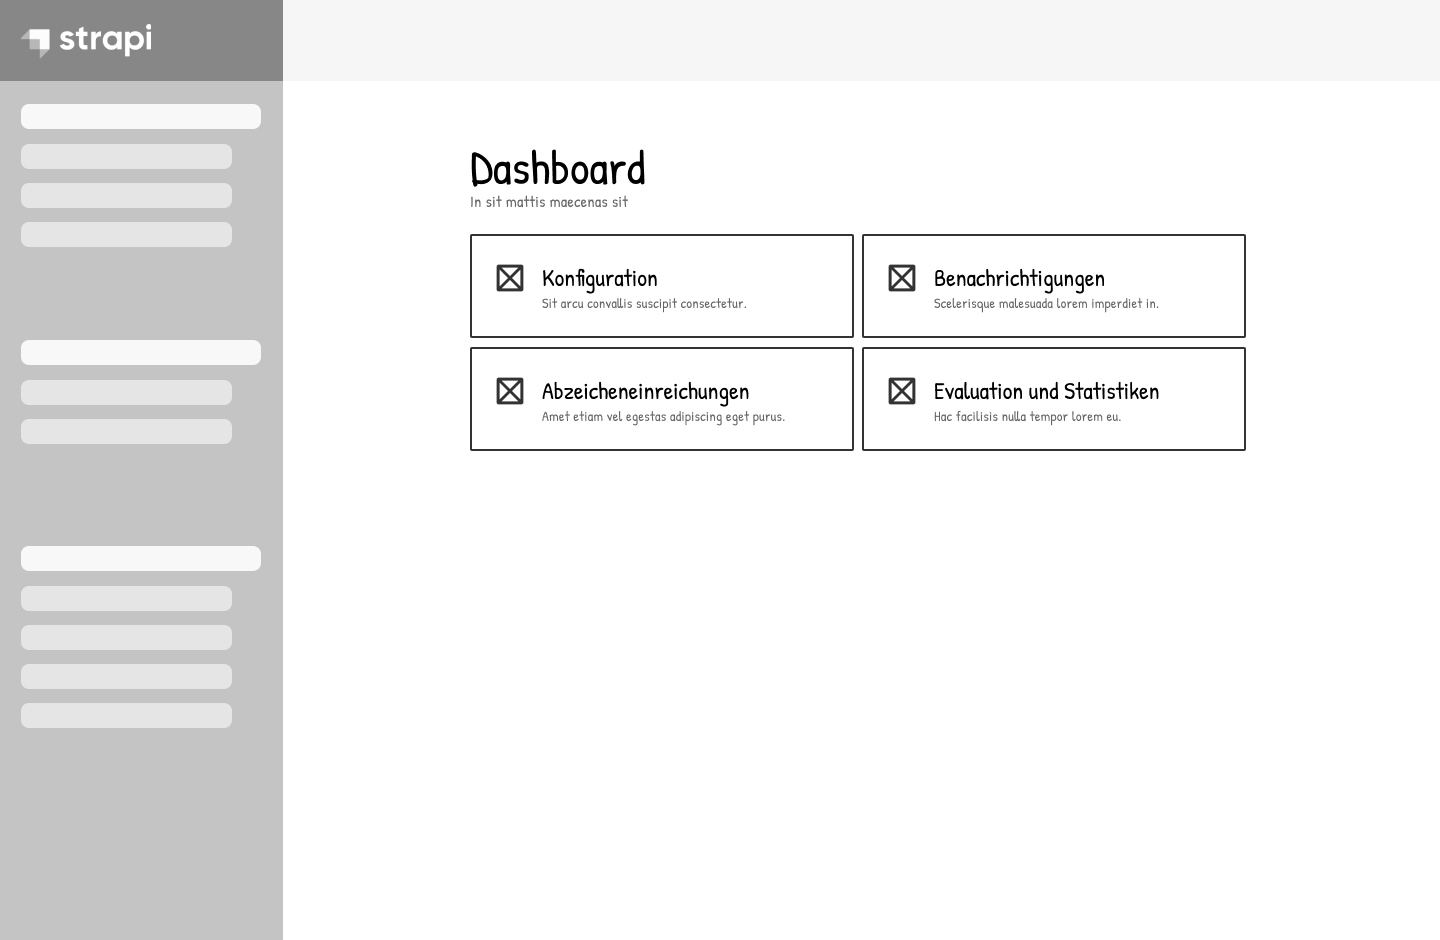
\includegraphics[width=\linewidth]{dialog/dashboard/dashboard.png}
    \caption{Dashboard - Starseite}
    \label{fig:dialog-v-home}
\end{figure}

Hierfür navigiert Sven zunächst zur Konfiguration aus
\autoref{fig:dialog-v-config}. Dort sieht er die verschiedenen Felder für Titel,
Logo, etc. und füllt diese für seine Veranstaltung aus. Außerdem entscheidet
Sven sich dazu, keine Gruppen in seiner Veranstaltung zuzulassen und schaltet
diese aus. Zudem möchte Sven nicht, dass jemand alles vor dem Start der
Veranstaltung sieht und im Internet verbreitet. Deswegen setzt er ein
entsprechendes Start-Datum.

\begin{figure}[htpb]
    \centering
    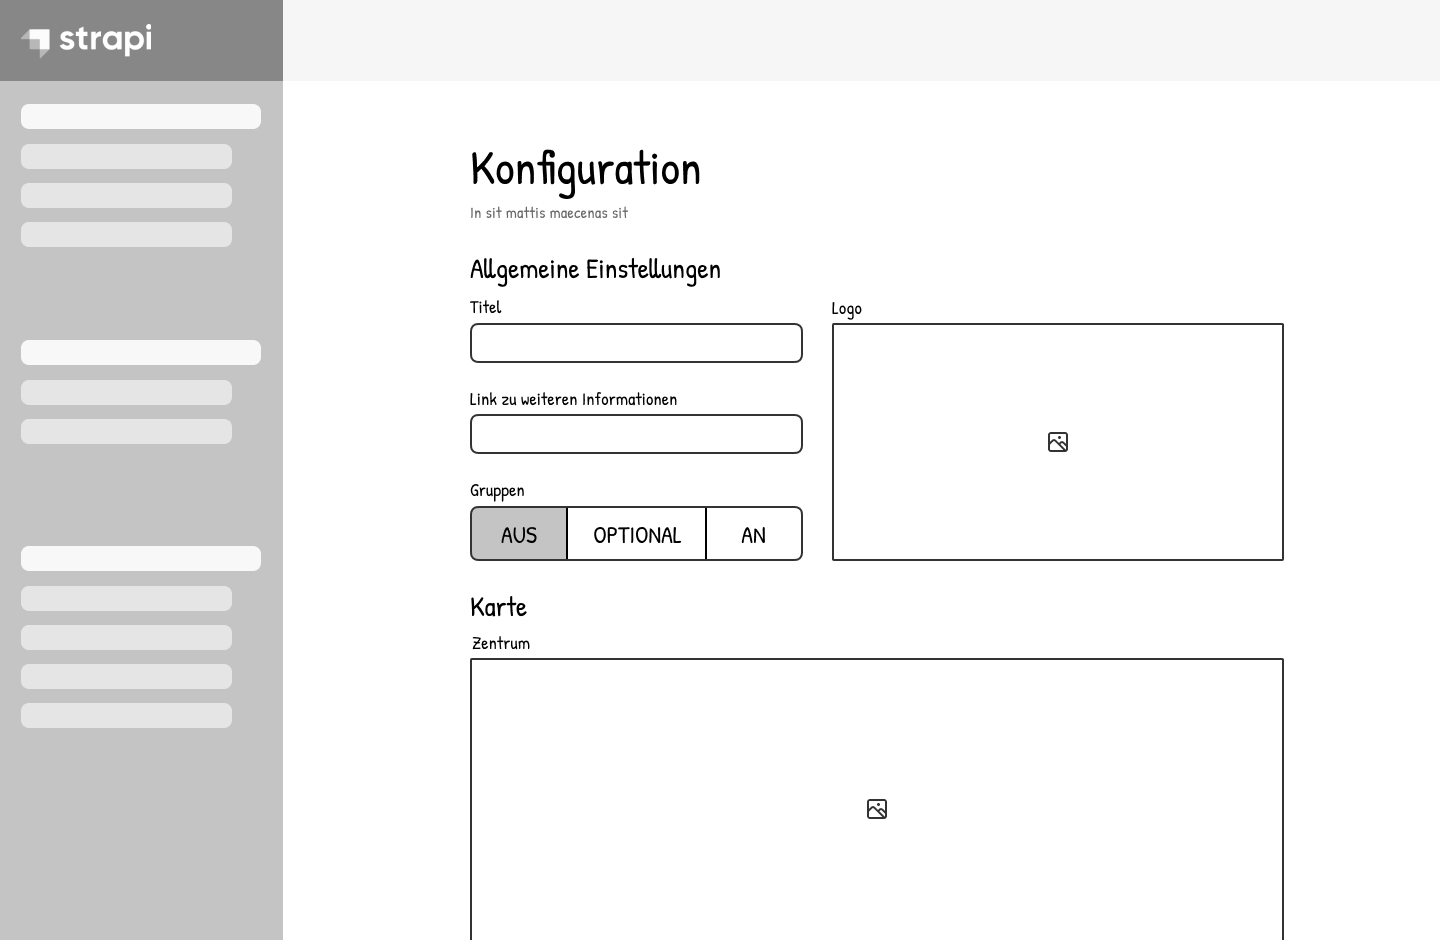
\includegraphics[width=\linewidth]{dialog/dashboard/configuration.png}
    \caption{Dashboard - Konfiguration der Rahmendaten}
    \label{fig:dialog-v-config}
\end{figure}

Am Start-Tag freut sich die junge Studentin Christina Müller bereits die
verschiedenen „Technology Bits“ zu besuchen. Als es so weit ist, ruft sie die
Event-App unter der URL \textit{https://app.technology-bits.de} auf und wird mit
einer Einführung in die Veranstaltung begrüßt (\autoref{fig:dialog-t-intro}).
In dieser erfährt Christina, was sie in Svens Veranstaltung alles erwartet.
Schließlich muss Christina noch der Datenschutzerklärung zustimmen.

\begin{figure}[htpb]
    \centering
    \begin{minipage}{.325\textwidth}
        \centering
        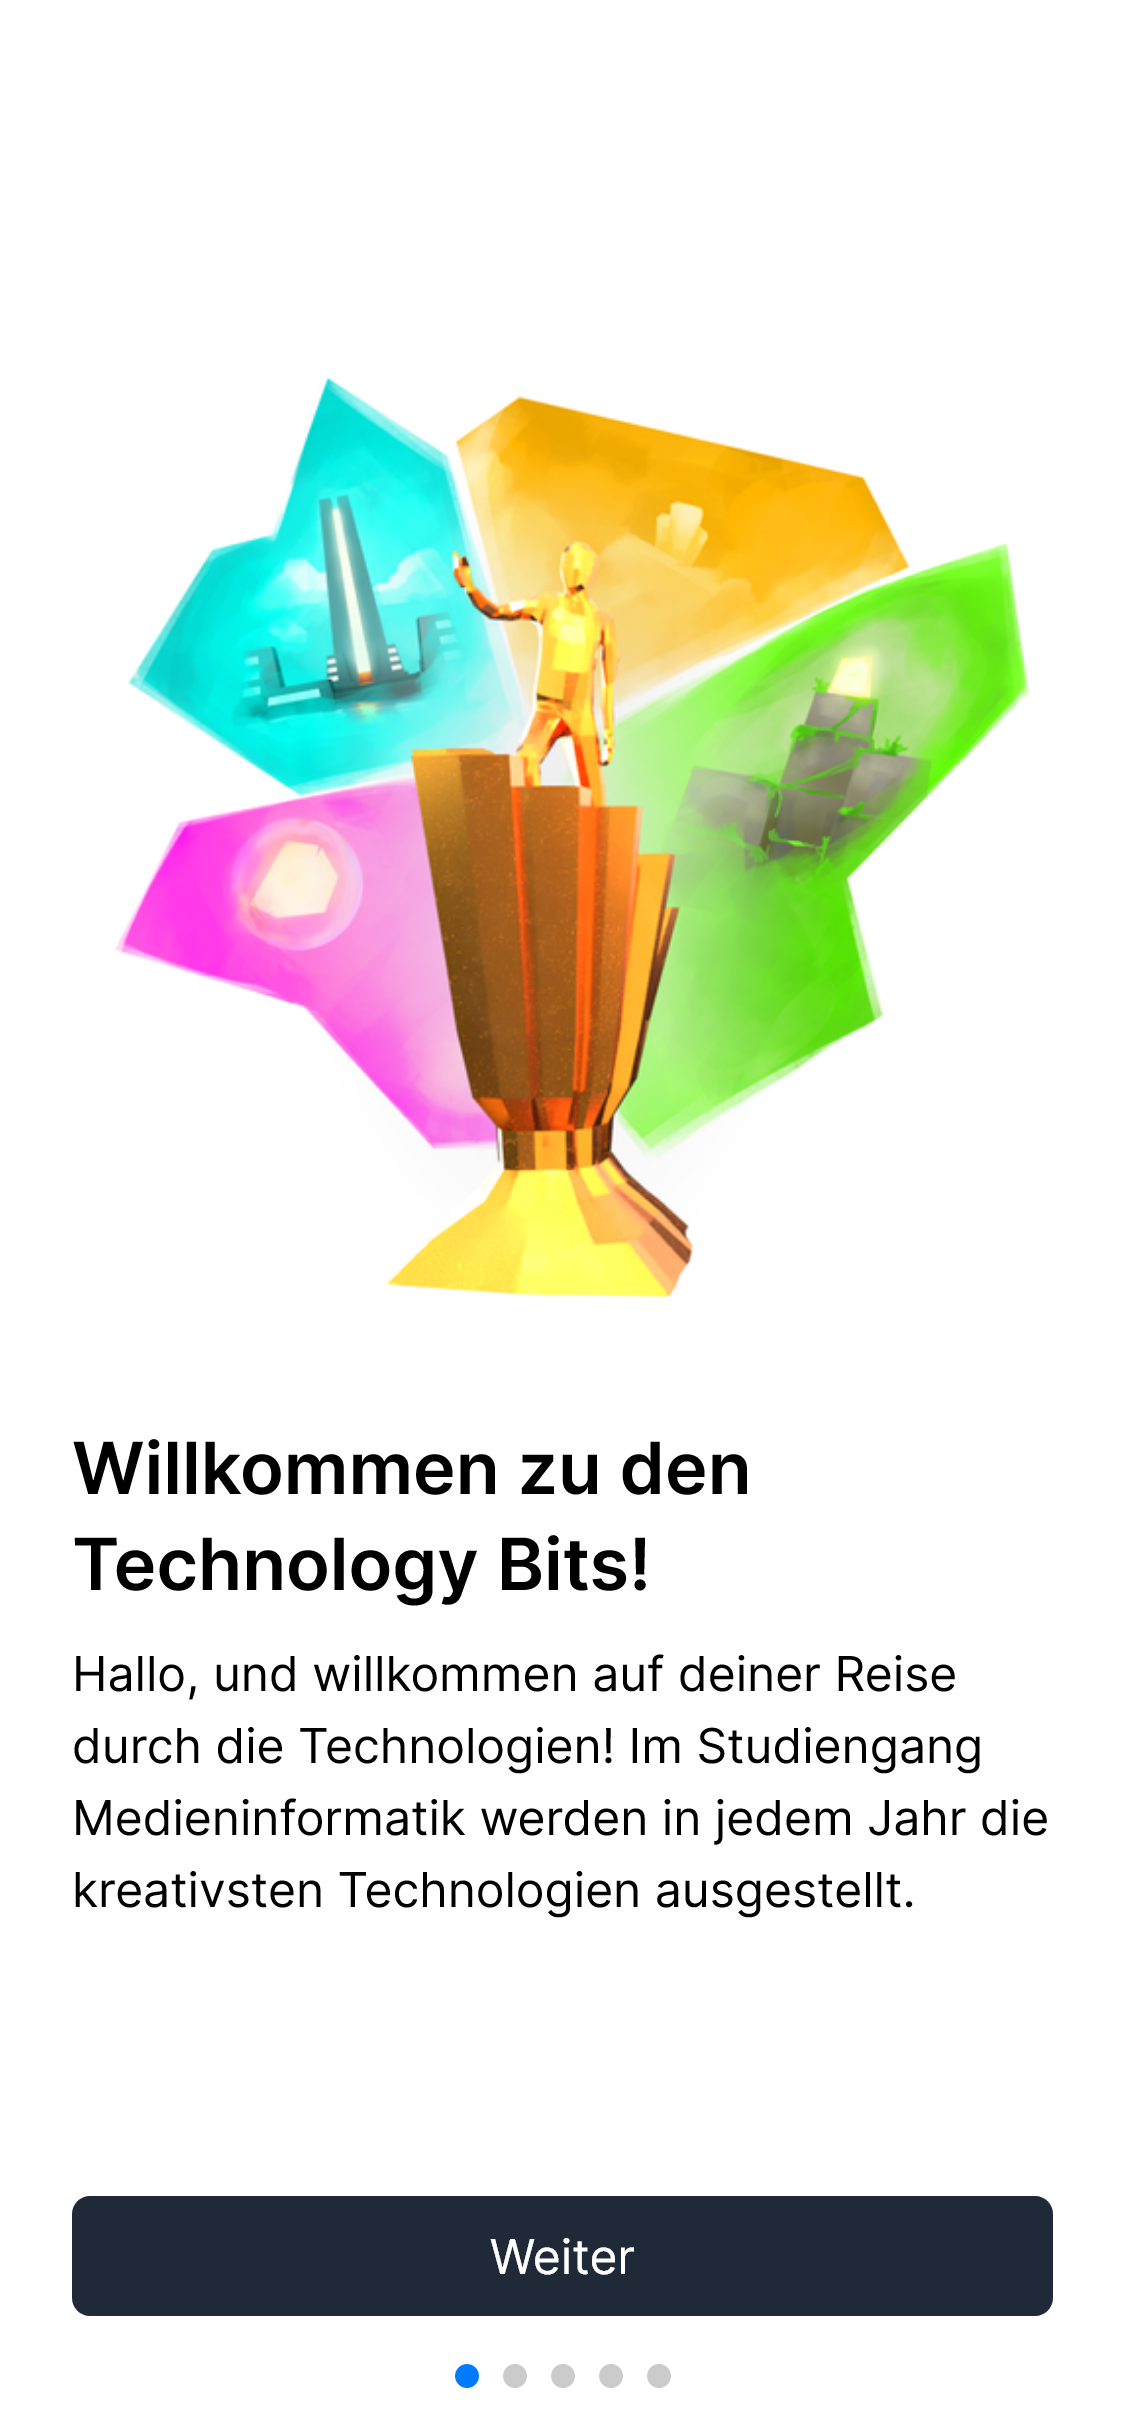
\includegraphics[width=.95\linewidth]{dialog/app/intro_title.png}
    \end{minipage}%
    \begin{minipage}{.325\textwidth}
        \centering
        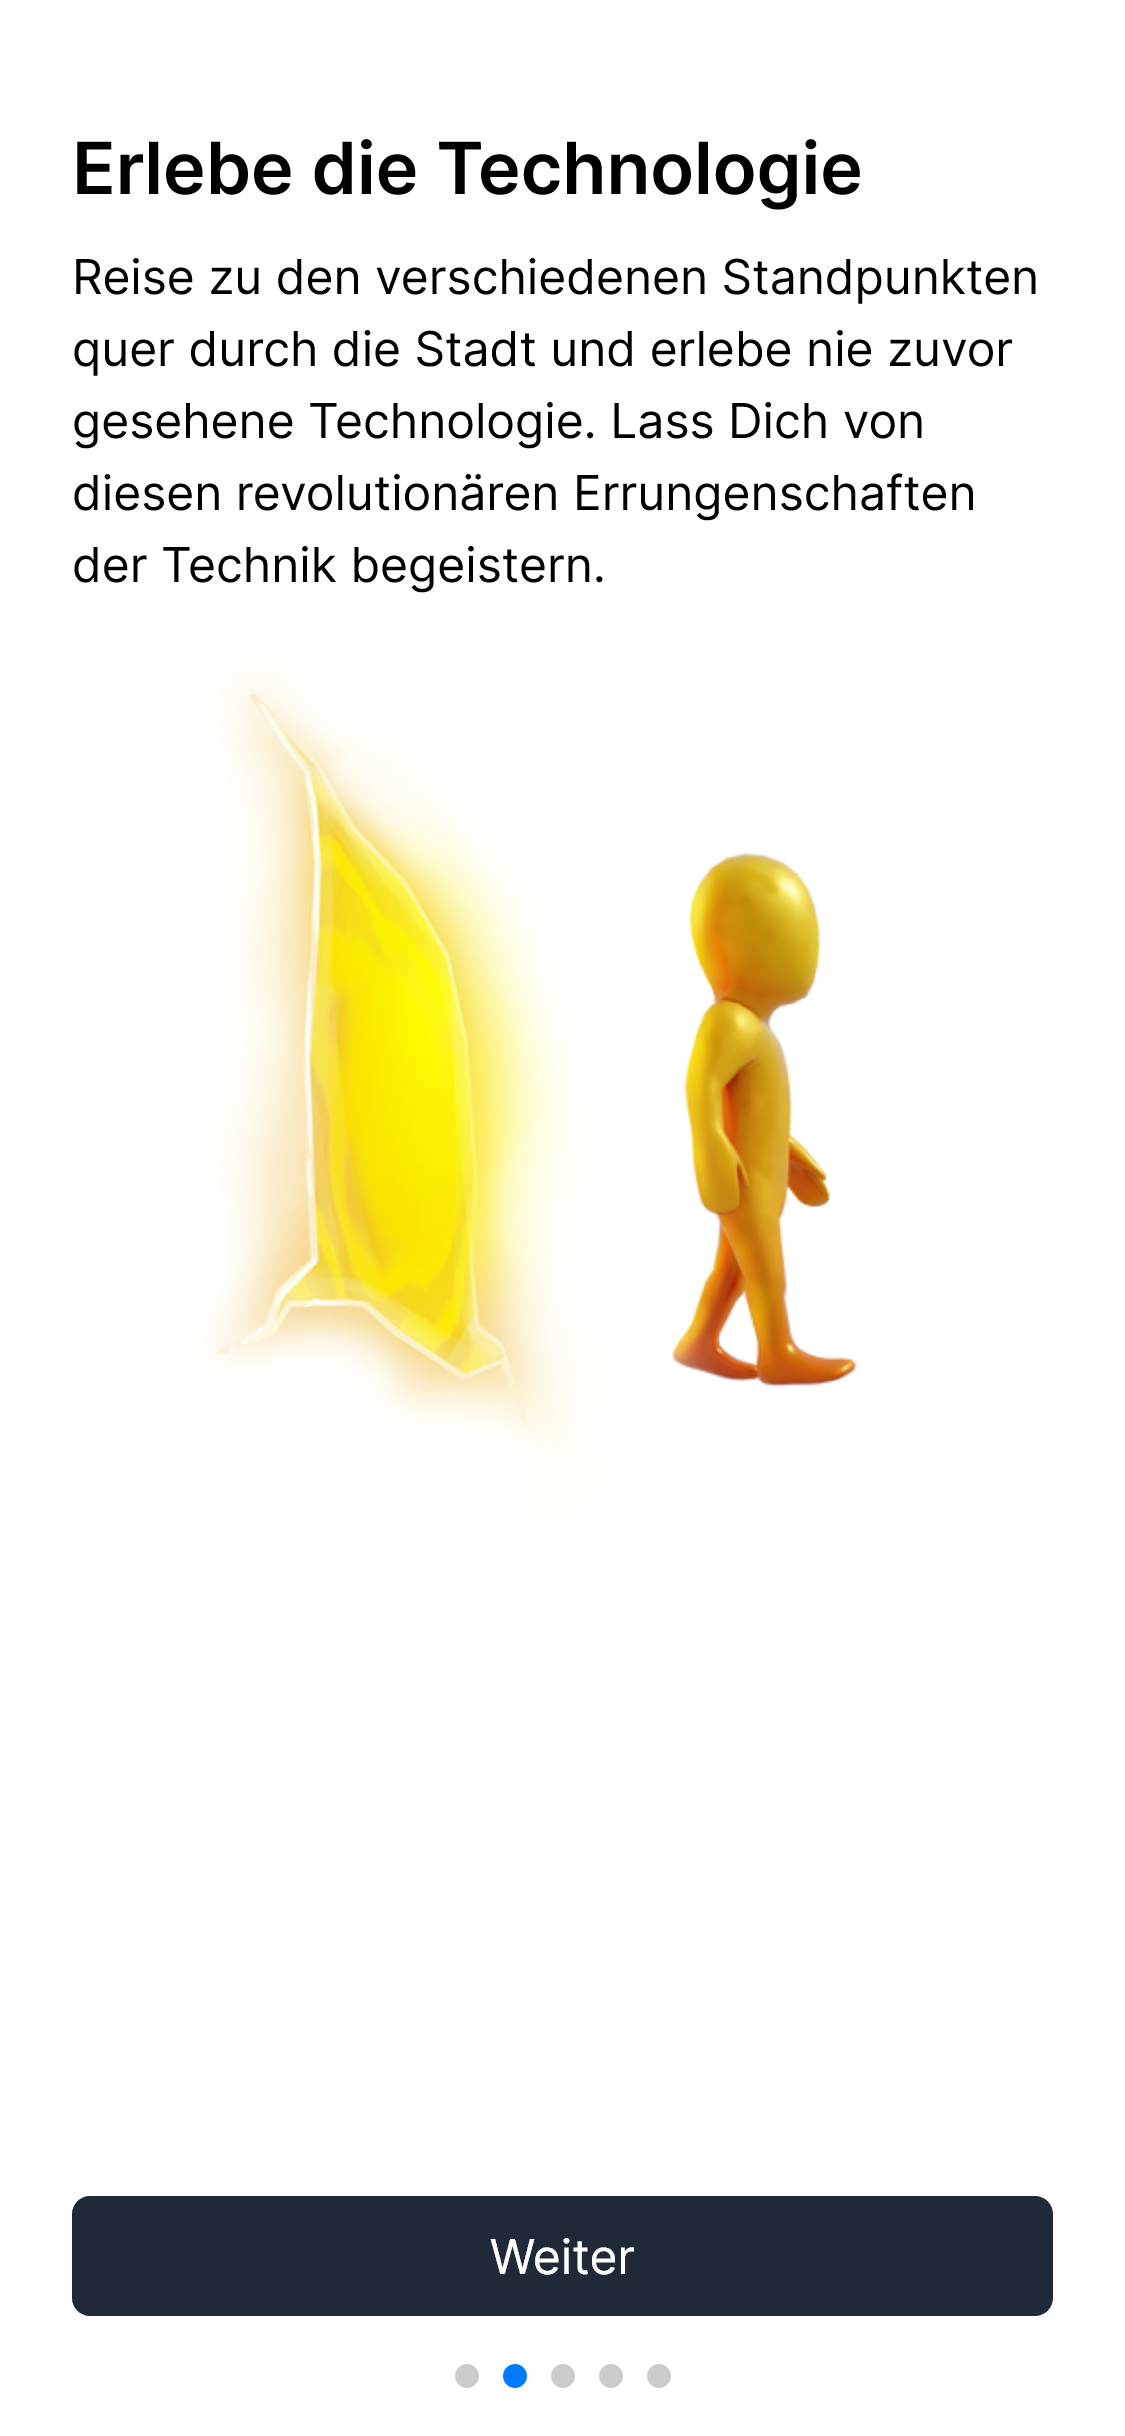
\includegraphics[width=.95\linewidth]{dialog/app/intro_image.png}
    \end{minipage}
    \begin{minipage}{.325\textwidth}
        \centering
        
\includegraphics[width=.95\linewidth]{dialog/app/intro_data.png}
    \end{minipage}
    \caption{Web-App - Einführung in die Veranstaltung}
    \label{fig:dialog-t-intro}
\end{figure}

Nachdem Christina zustimmt, wird sie endlich zur Karte weitergeleitet (\autoref{fig:dialog-t-map}). Auf dieser sieht sie die verschiedenen Stationen,
welche quer in der Stadt verteilt sind. Sie entschließt sich eine zufällige
Station auszuwählen und landet auf „Sparfuchs“. Bei diesem Namen wundert sie
sich, was für eine Technologie dahintersteckt und tippt auf „Mehr Erfahren“.
Hier sieht sie zur ihrer Enttäuschung, dass sie die Station erst besuchen muss,
wenn sie mehr zu ihr erfahren möchte. Folglich macht sich Christina auf den Weg
zur Station.

\begin{figure}[htpb]
    \centering
    \begin{minipage}{.325\textwidth}
        \centering
        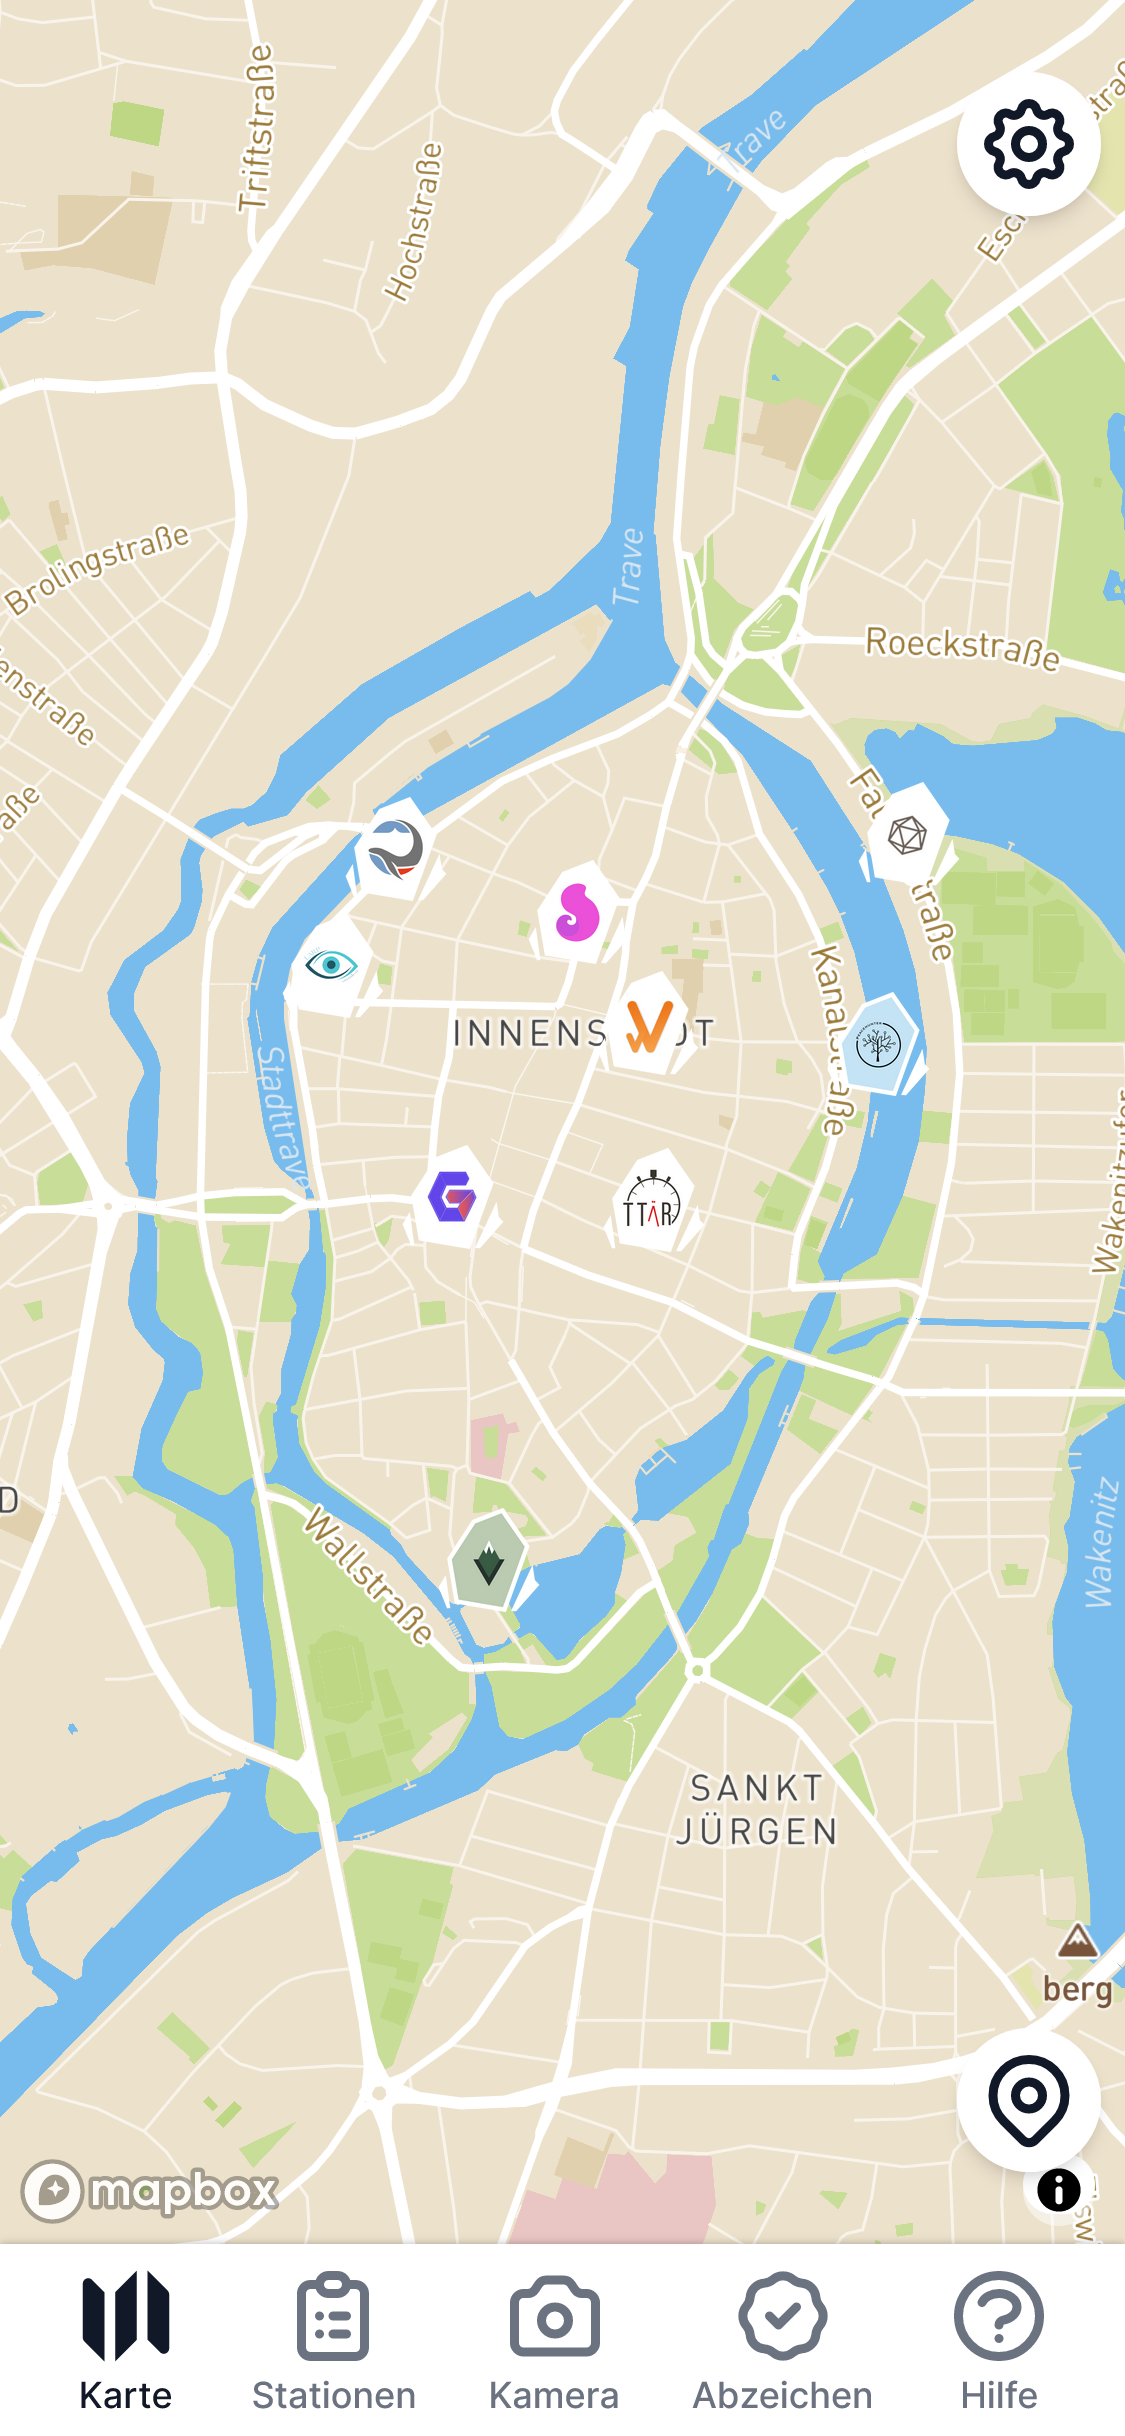
\includegraphics[width=.95\linewidth]{dialog/app/map.png}
    \end{minipage}%
    \begin{minipage}{.325\textwidth}
        \centering
        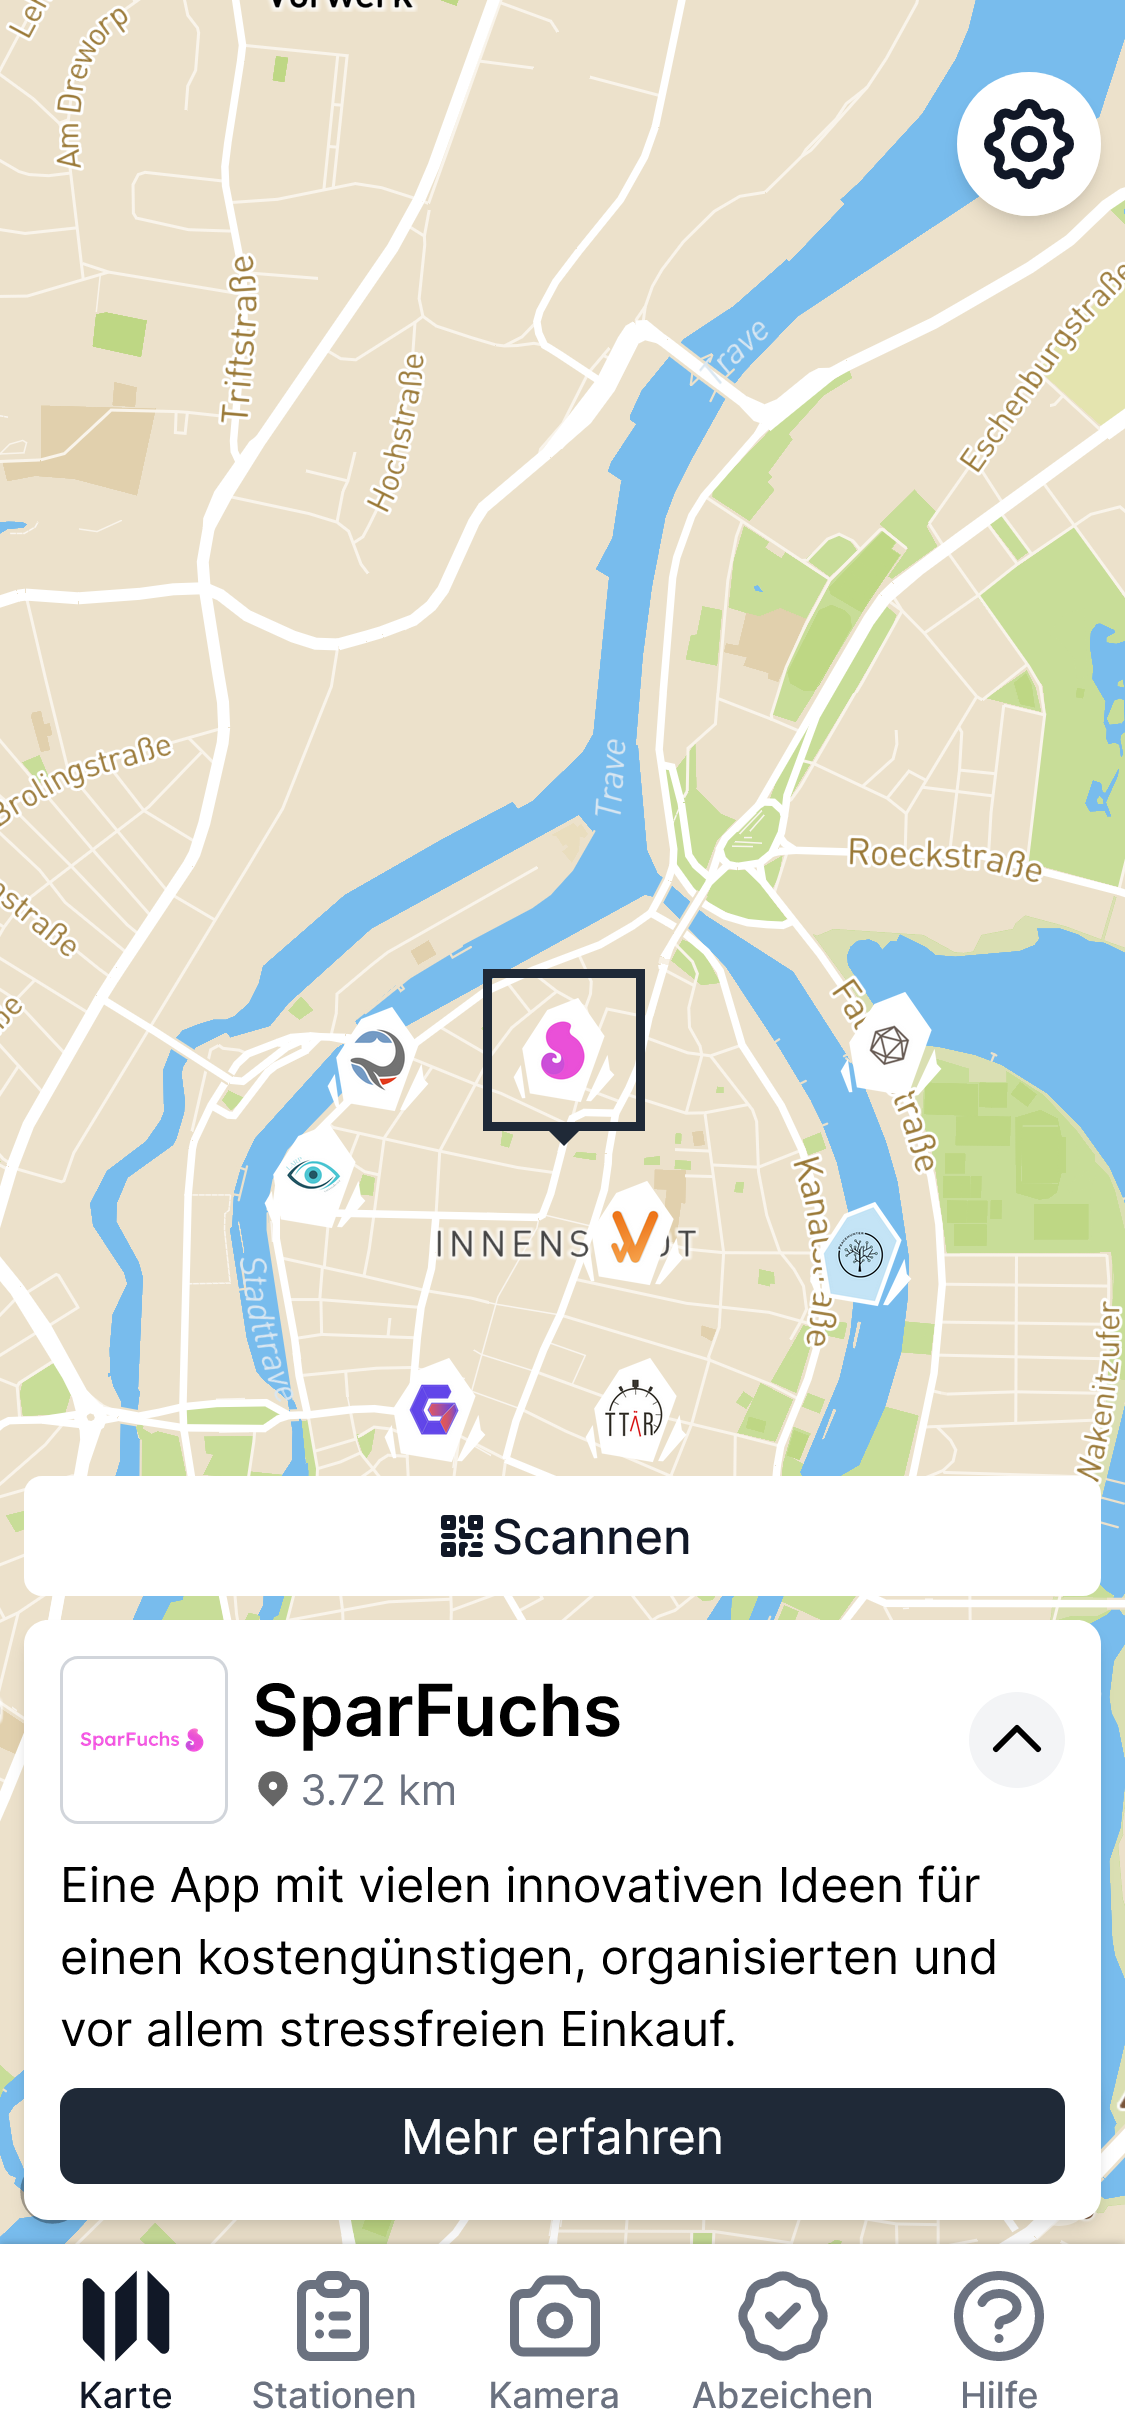
\includegraphics[width=.95\linewidth]{dialog/app/map_selected.png}
    \end{minipage}
    \begin{minipage}{.325\textwidth}
        \centering
        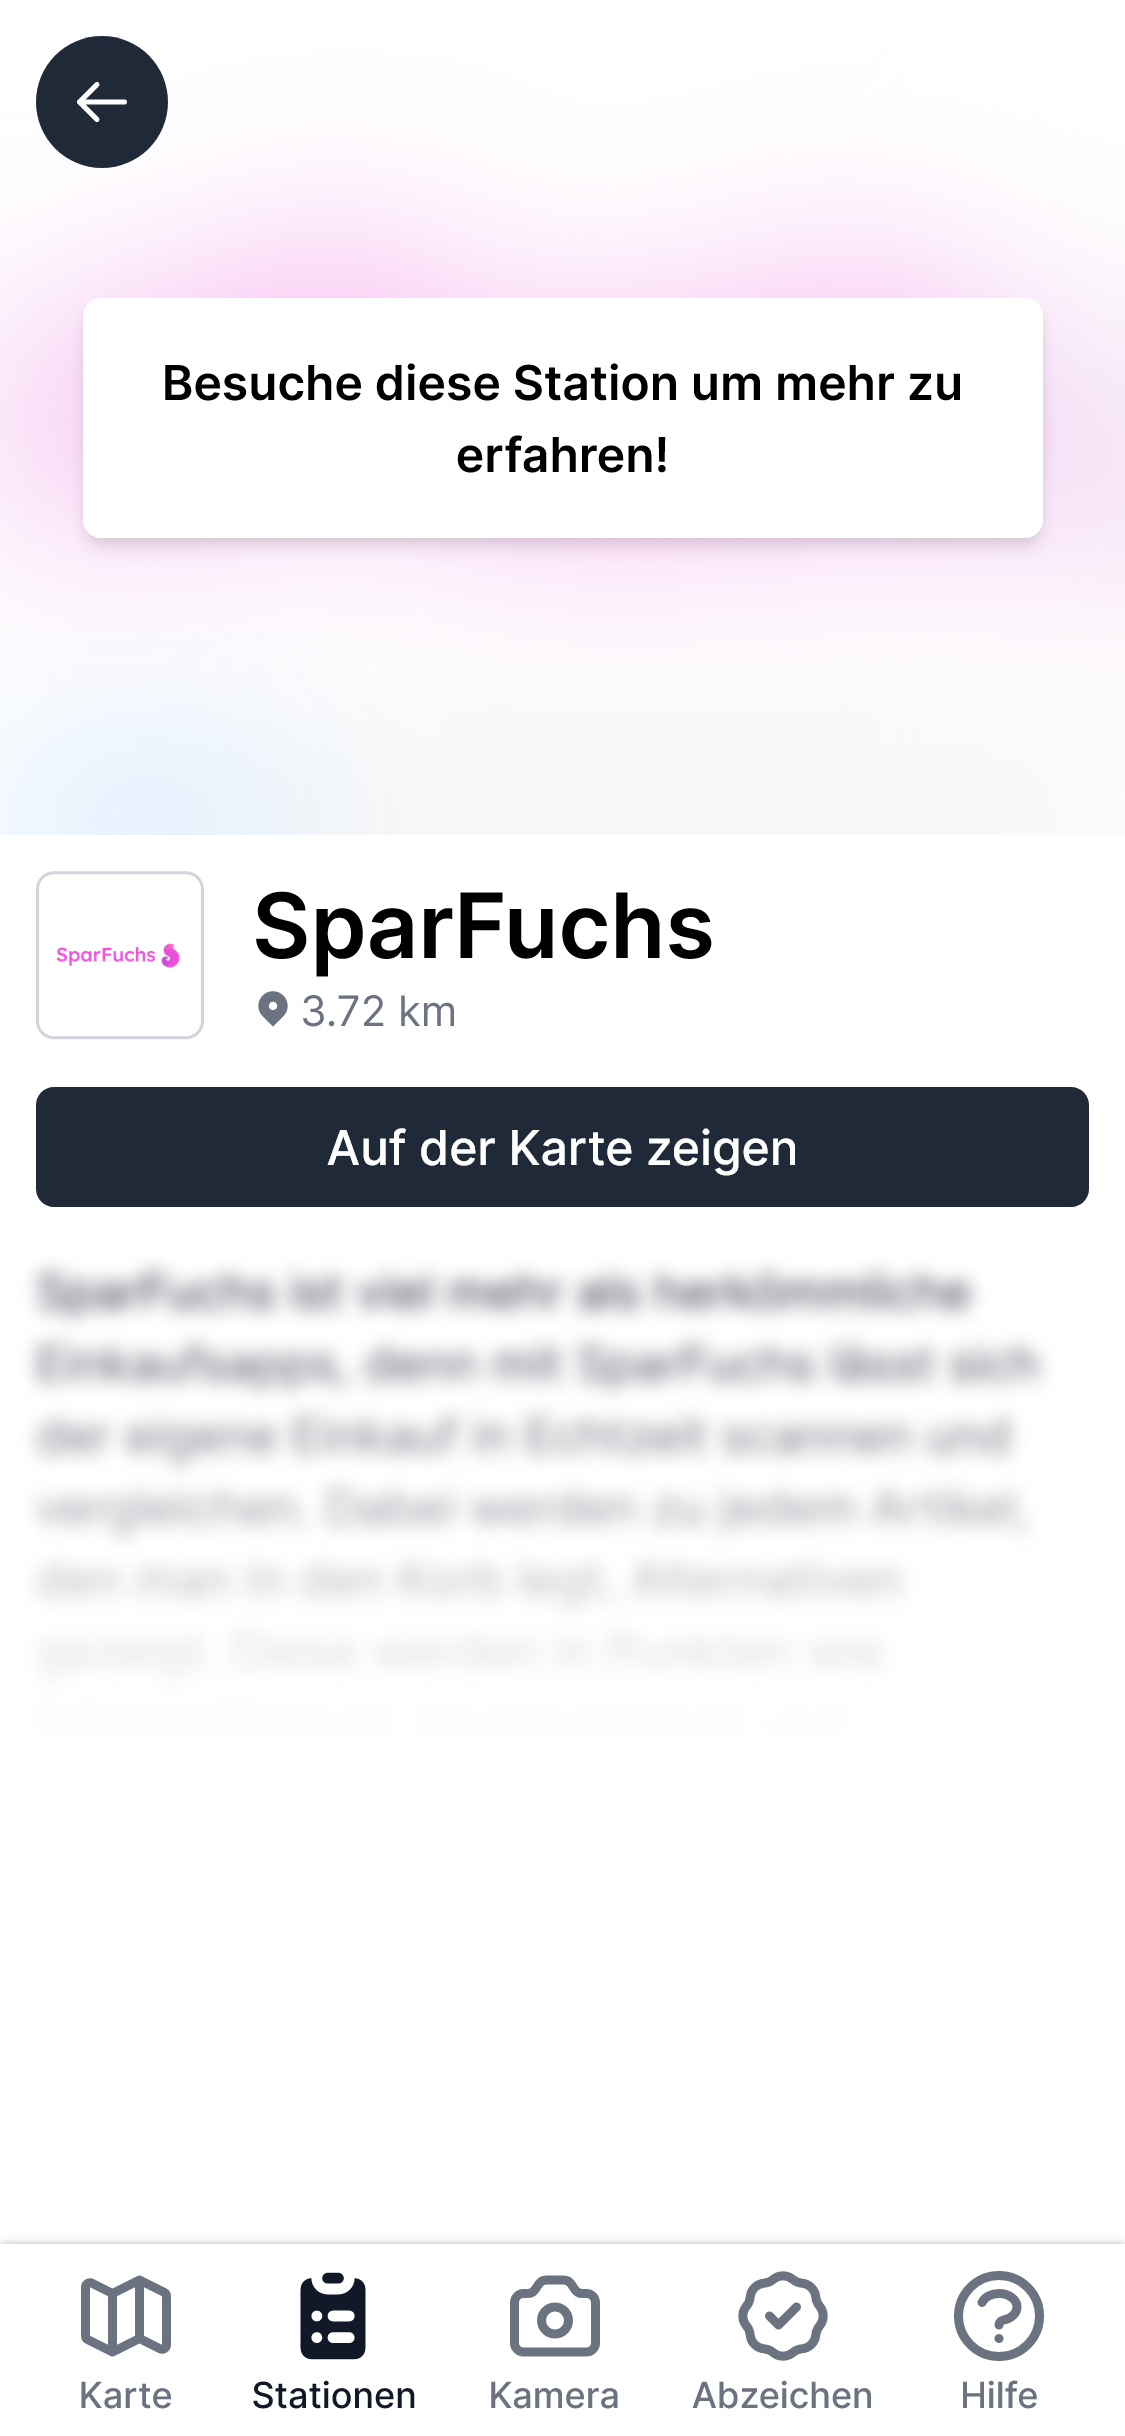
\includegraphics[width=.95\linewidth]{dialog/app/station_hidden.png}
    \end{minipage}
    \caption{Web-App - Interaktive Karte und Station}
    \label{fig:dialog-t-map}
\end{figure}

Dort angekommen öffnet Christina die Kamera der App (\autoref{fig:dialog-t-visit}) und versucht den dort angebrachten QR-Code zu
scannen. Leider hat Sven beim Druck nicht aufgepasst und einen ungültigen
QR-Code gedruckt. Christina ist sich nicht sicher, was sie machen soll und tippt
auf das Fragezeichen. Hier sieht sie die Möglichkeit den Code der Station so
einzugeben. Dieser ist ihr bereits unter dem angebrachten QR-Code aufgefallen.
Christina tippt somit auf „Code eingeben“ und trägt den ausgewiesenen Code ein.

\begin{figure}[htpb]
    \centering
    \begin{minipage}{.325\textwidth}
        \centering
        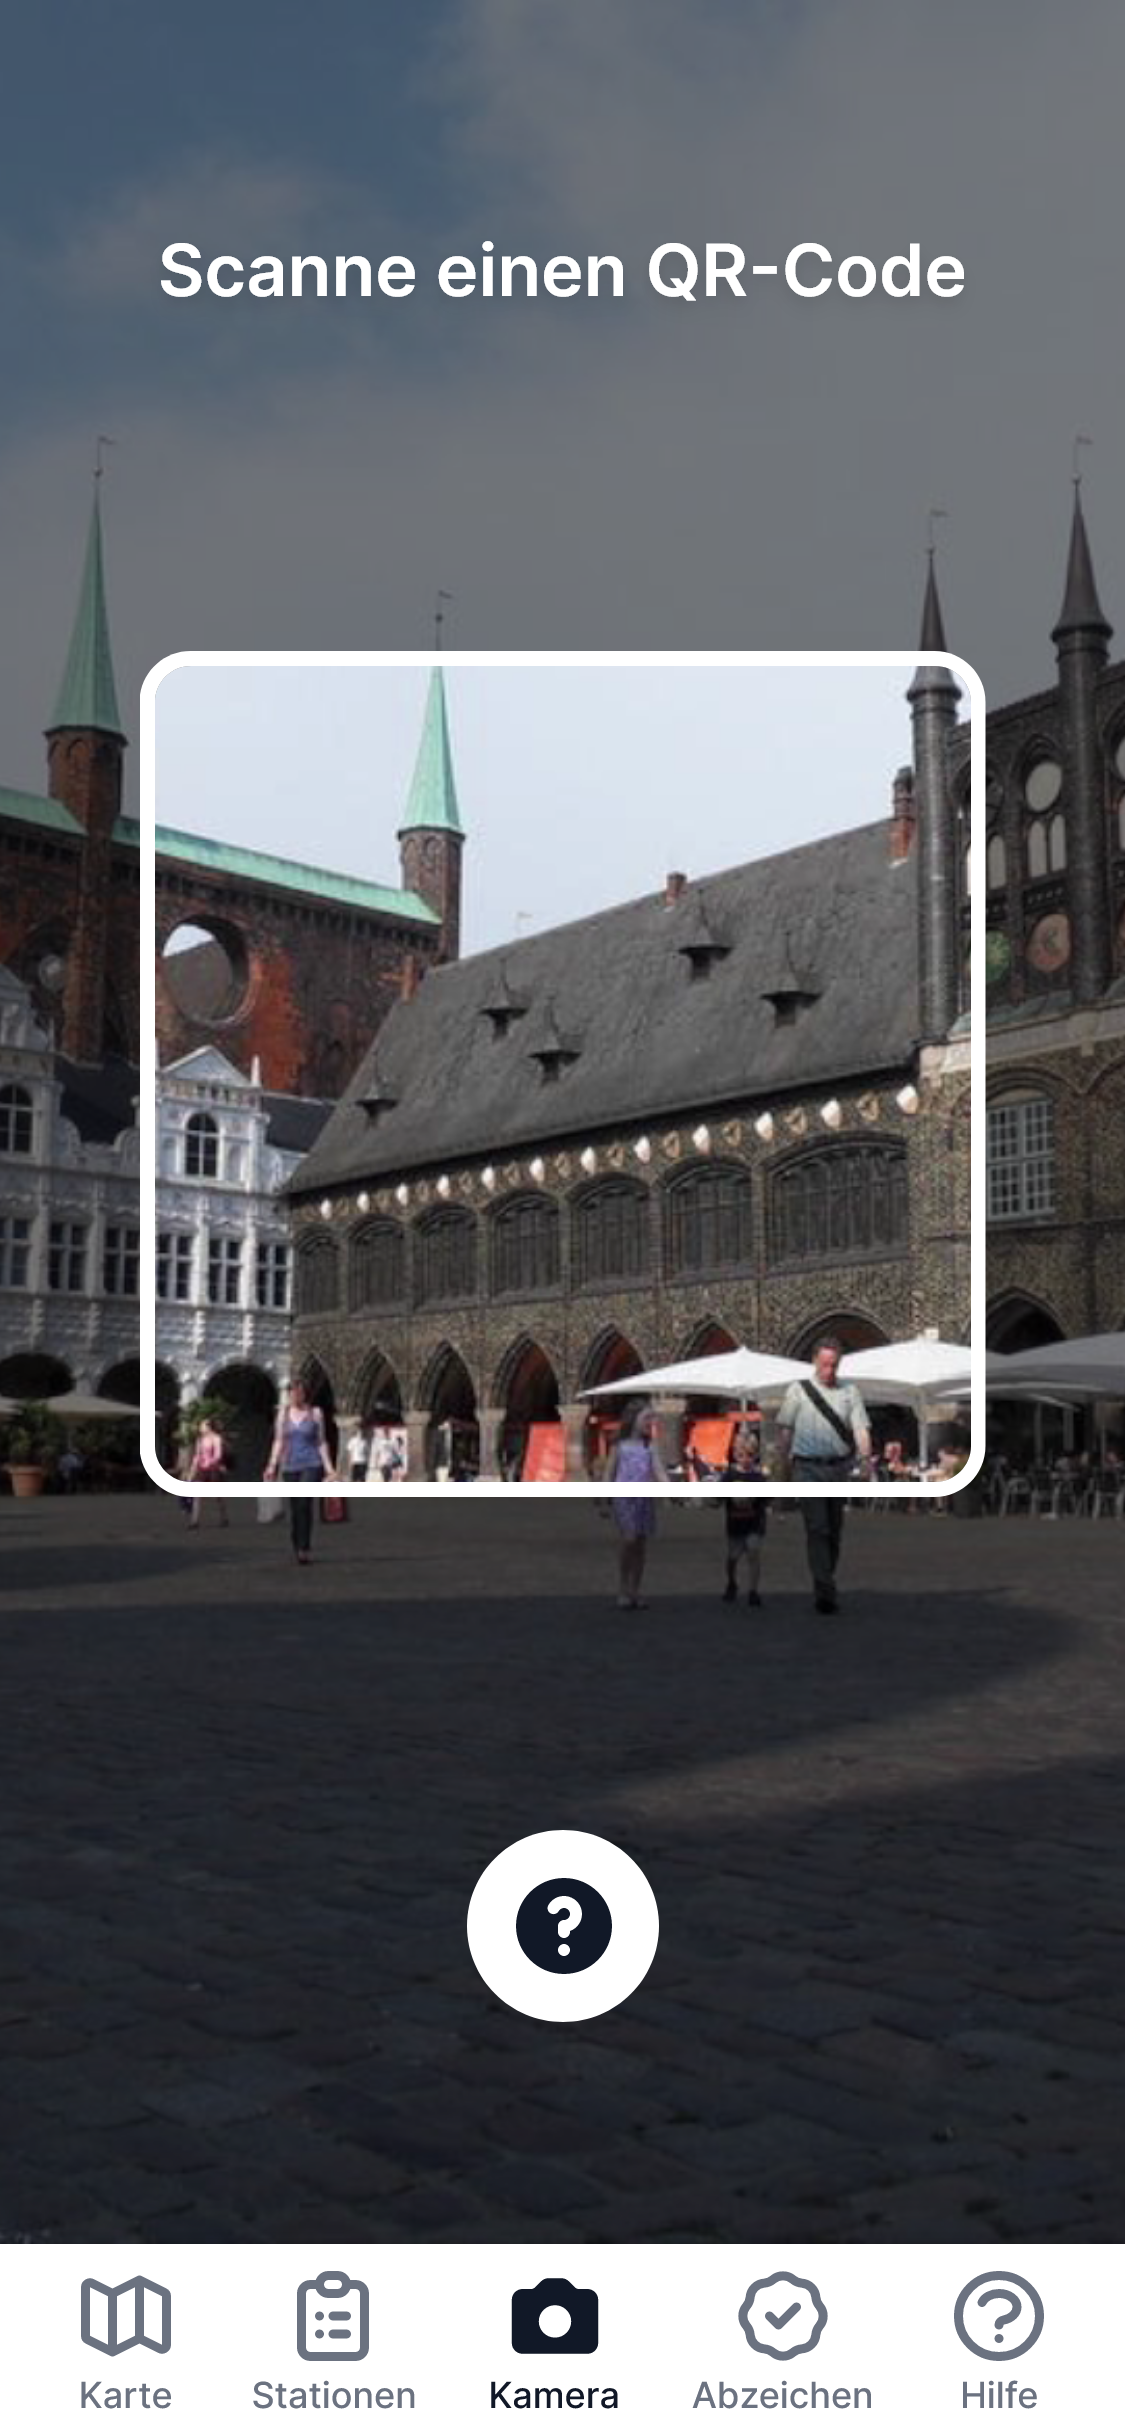
\includegraphics[width=.95\linewidth]{dialog/app/camera.png}
    \end{minipage}%
    \begin{minipage}{.325\textwidth}
        \centering
        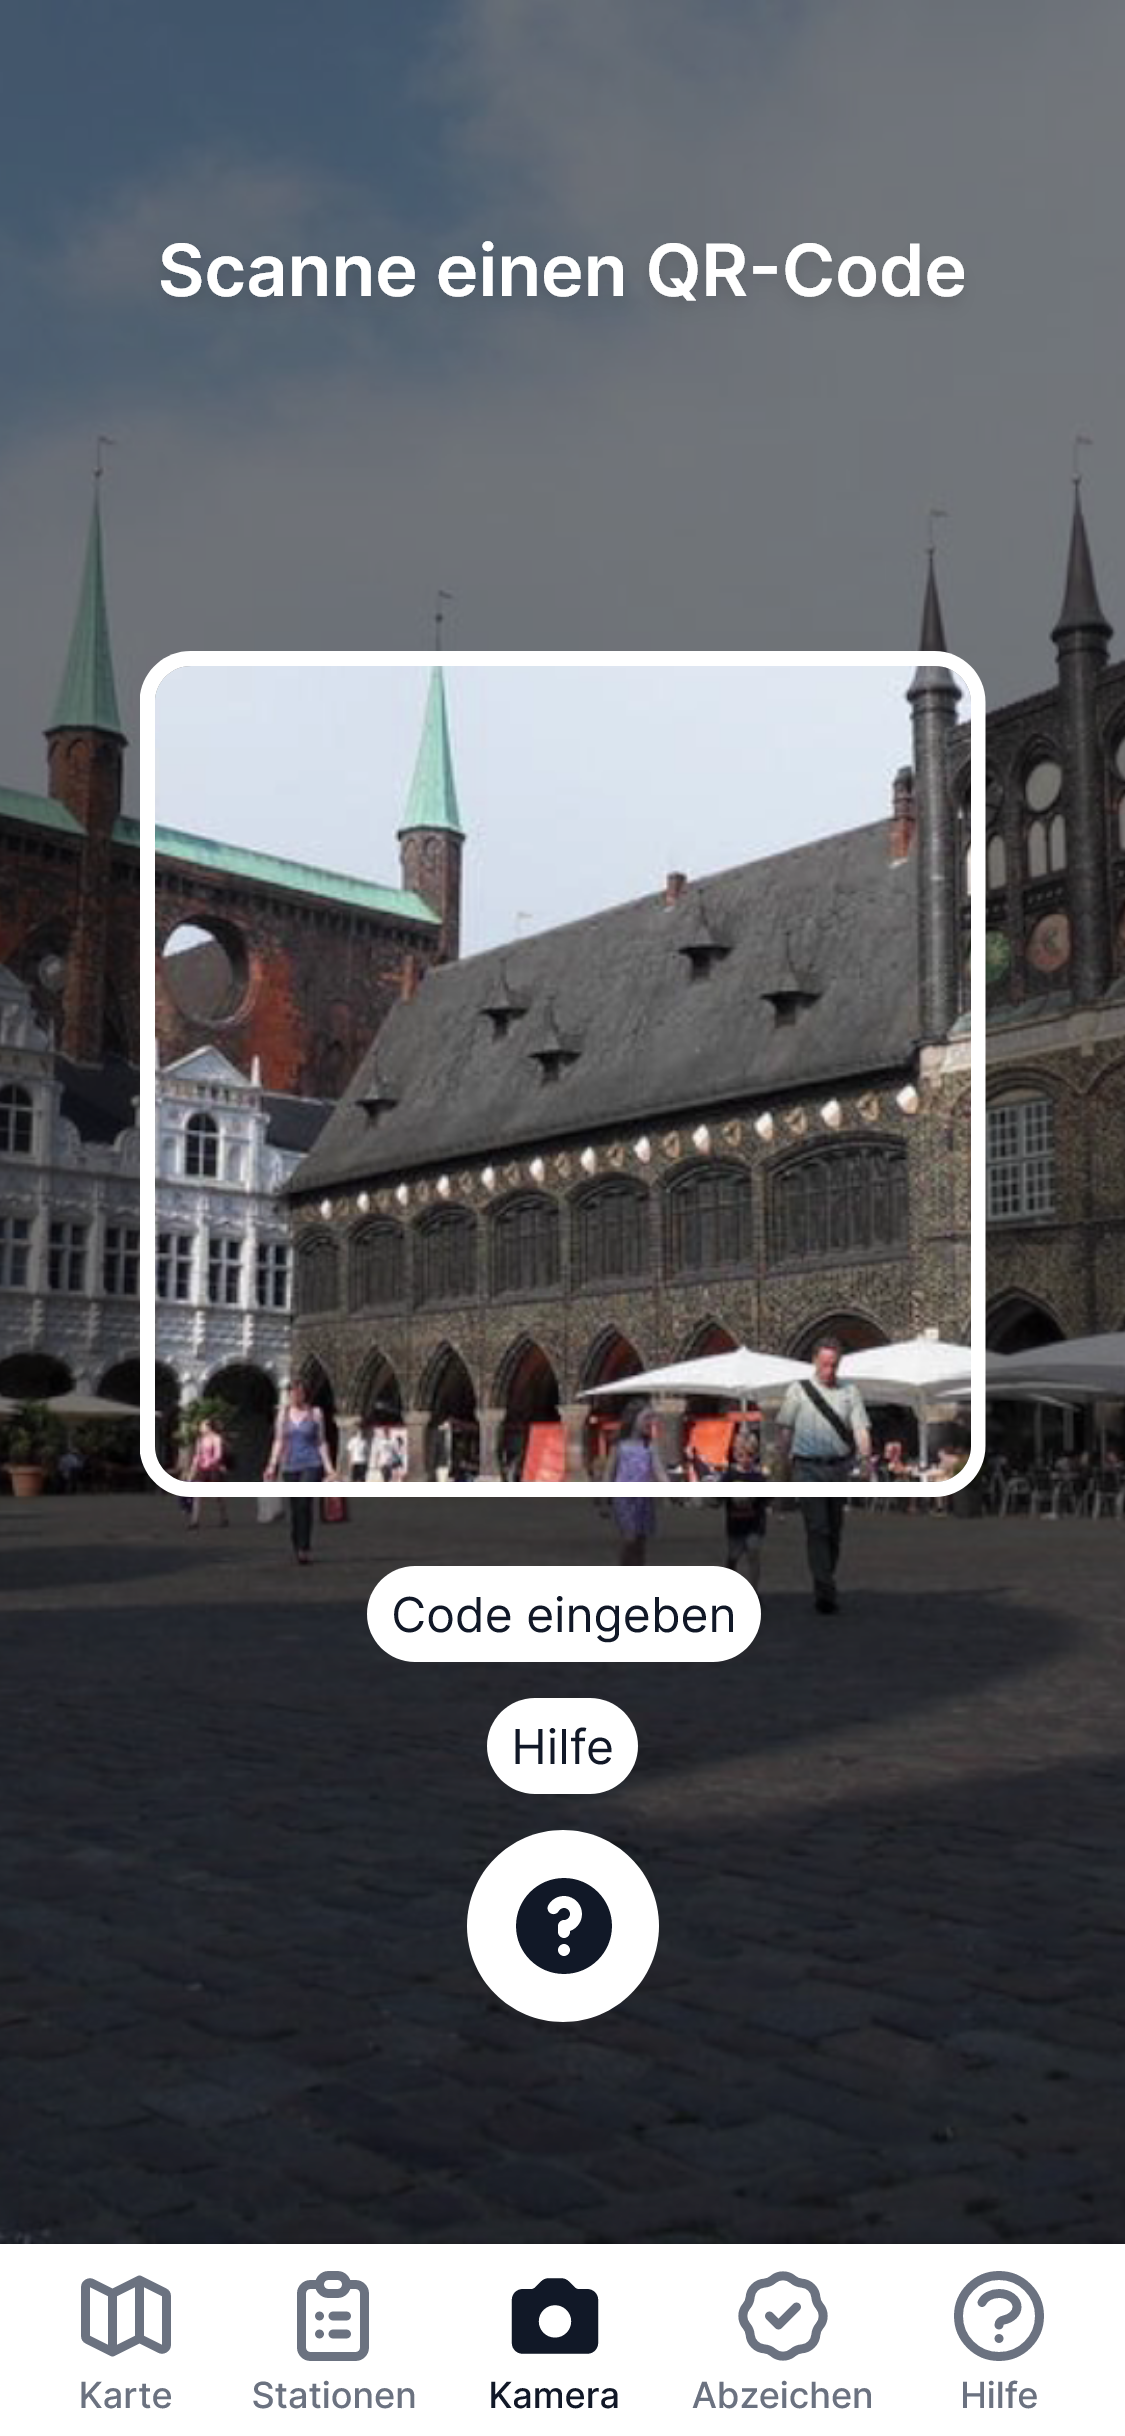
\includegraphics[width=.95\linewidth]{dialog/app/camera_speed-dial.png}
    \end{minipage}
    \begin{minipage}{.325\textwidth}
        \centering
        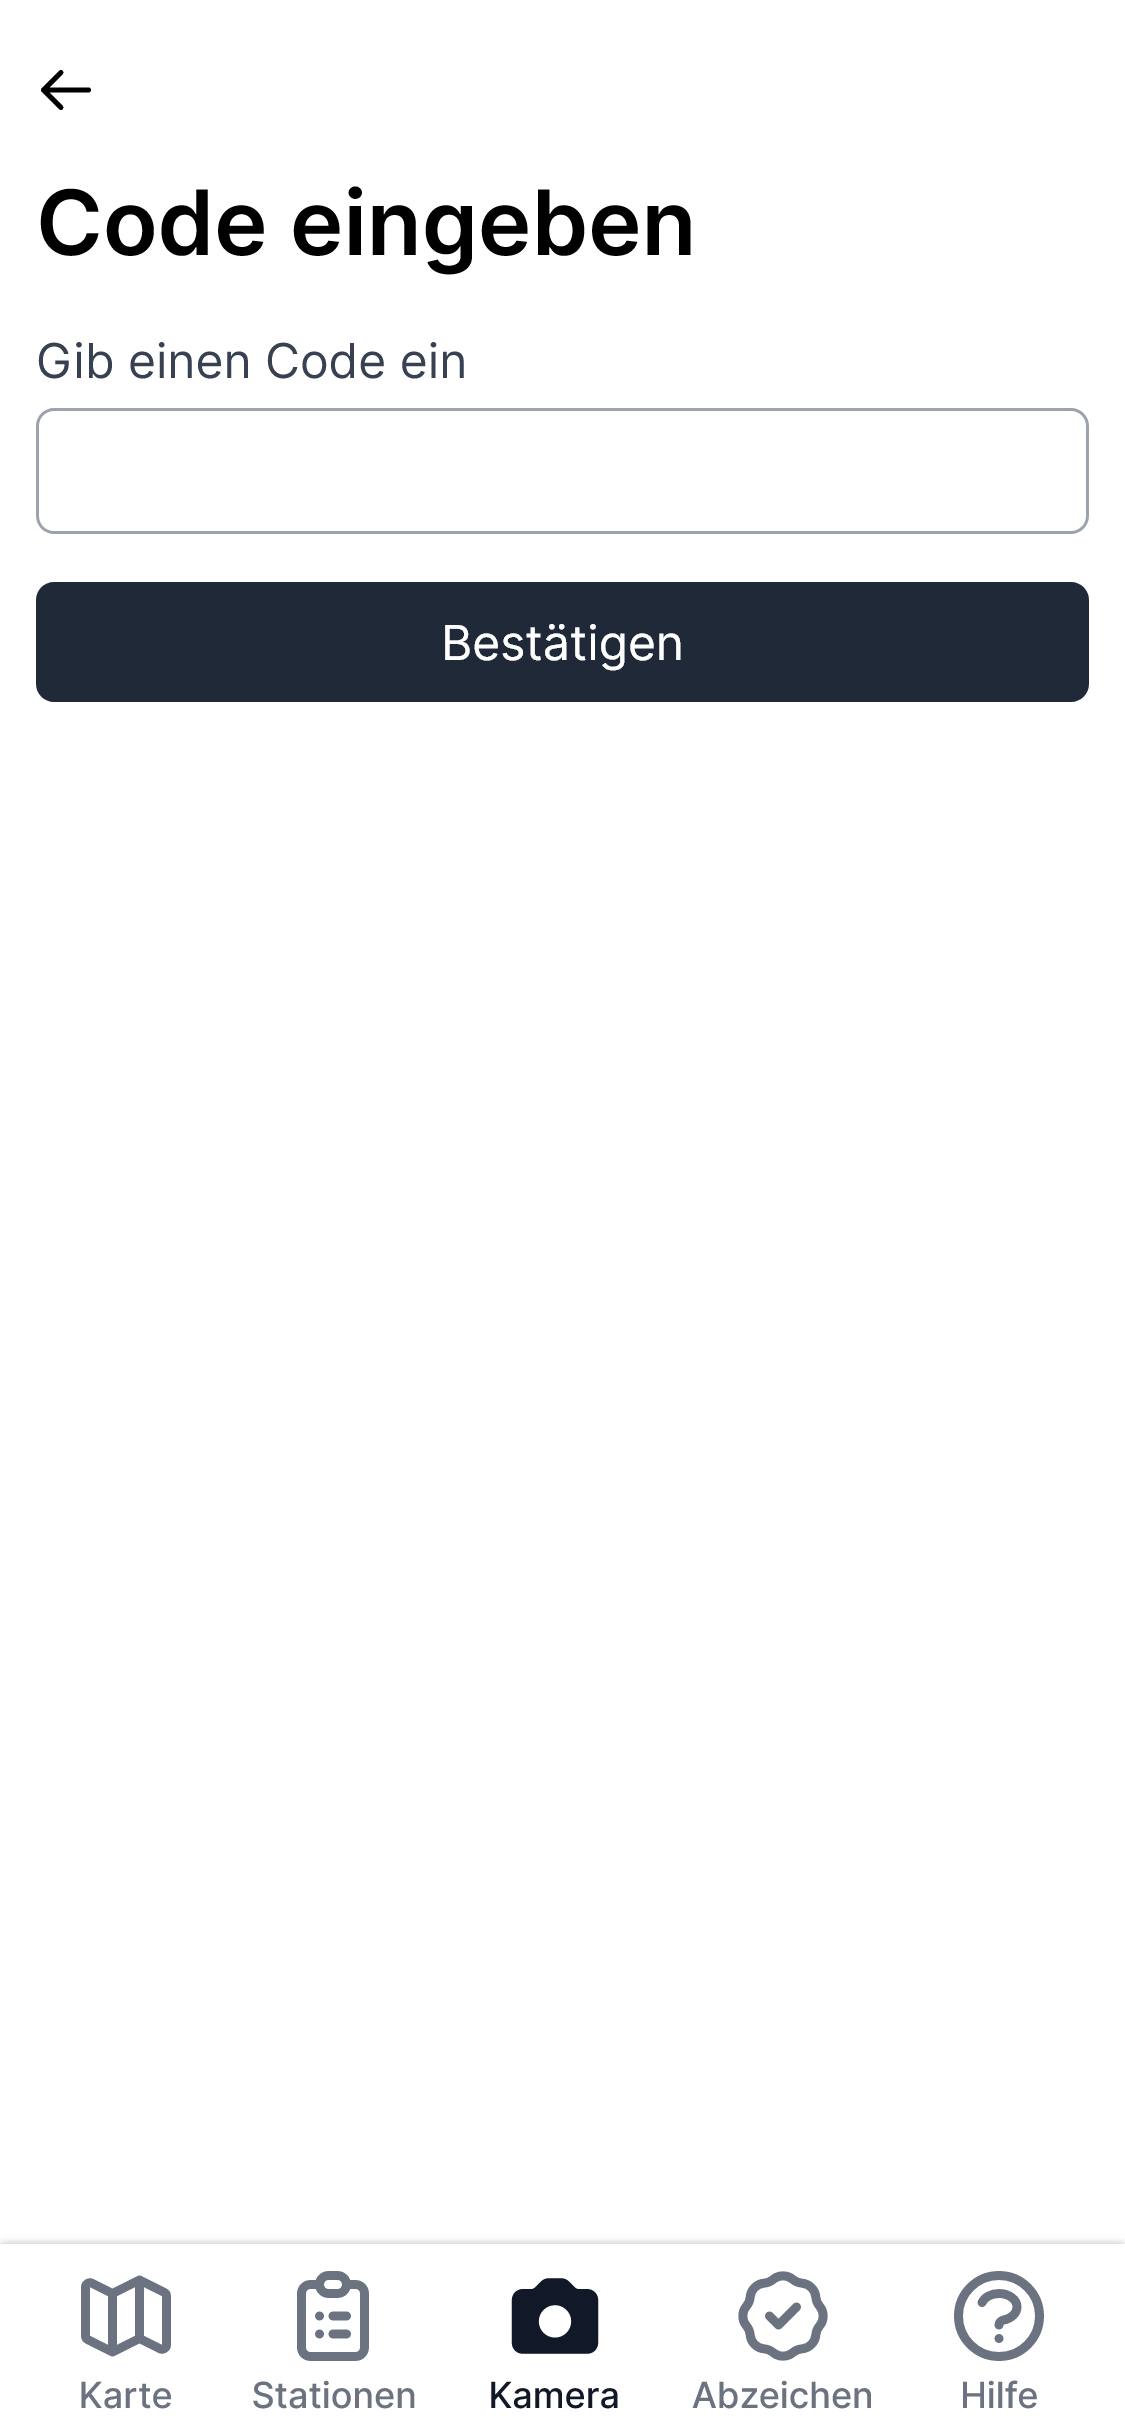
\includegraphics[width=.95\linewidth]{dialog/app/camera_code.png}
    \end{minipage}
    \caption{Web-App - Virtuelles Besuchen und Code Eingabe}
    \label{fig:dialog-t-visit}
\end{figure}

Mit dem Tippen auf „Bestätigen“ wechselt die App wieder zur Sparfuchs Station
(\autoref{fig:dialog-t-station-visited}). Jedoch kann Christina sich nun
endlich anschauen, was hinter dem Namen der Station steckt. Da sie jetzt schon
in der Stadt ist, entschließt sie sich gleich noch ein paar weitere Stationen zu
besuchen. Um die nächstgelegene Station zu sehen, wechselt sie hierfür zur
Stationsliste und besucht nach und nach einige Stationen.

\begin{figure}[htpb]
    \centering
    \begin{minipage}{.325\textwidth}
        \centering
        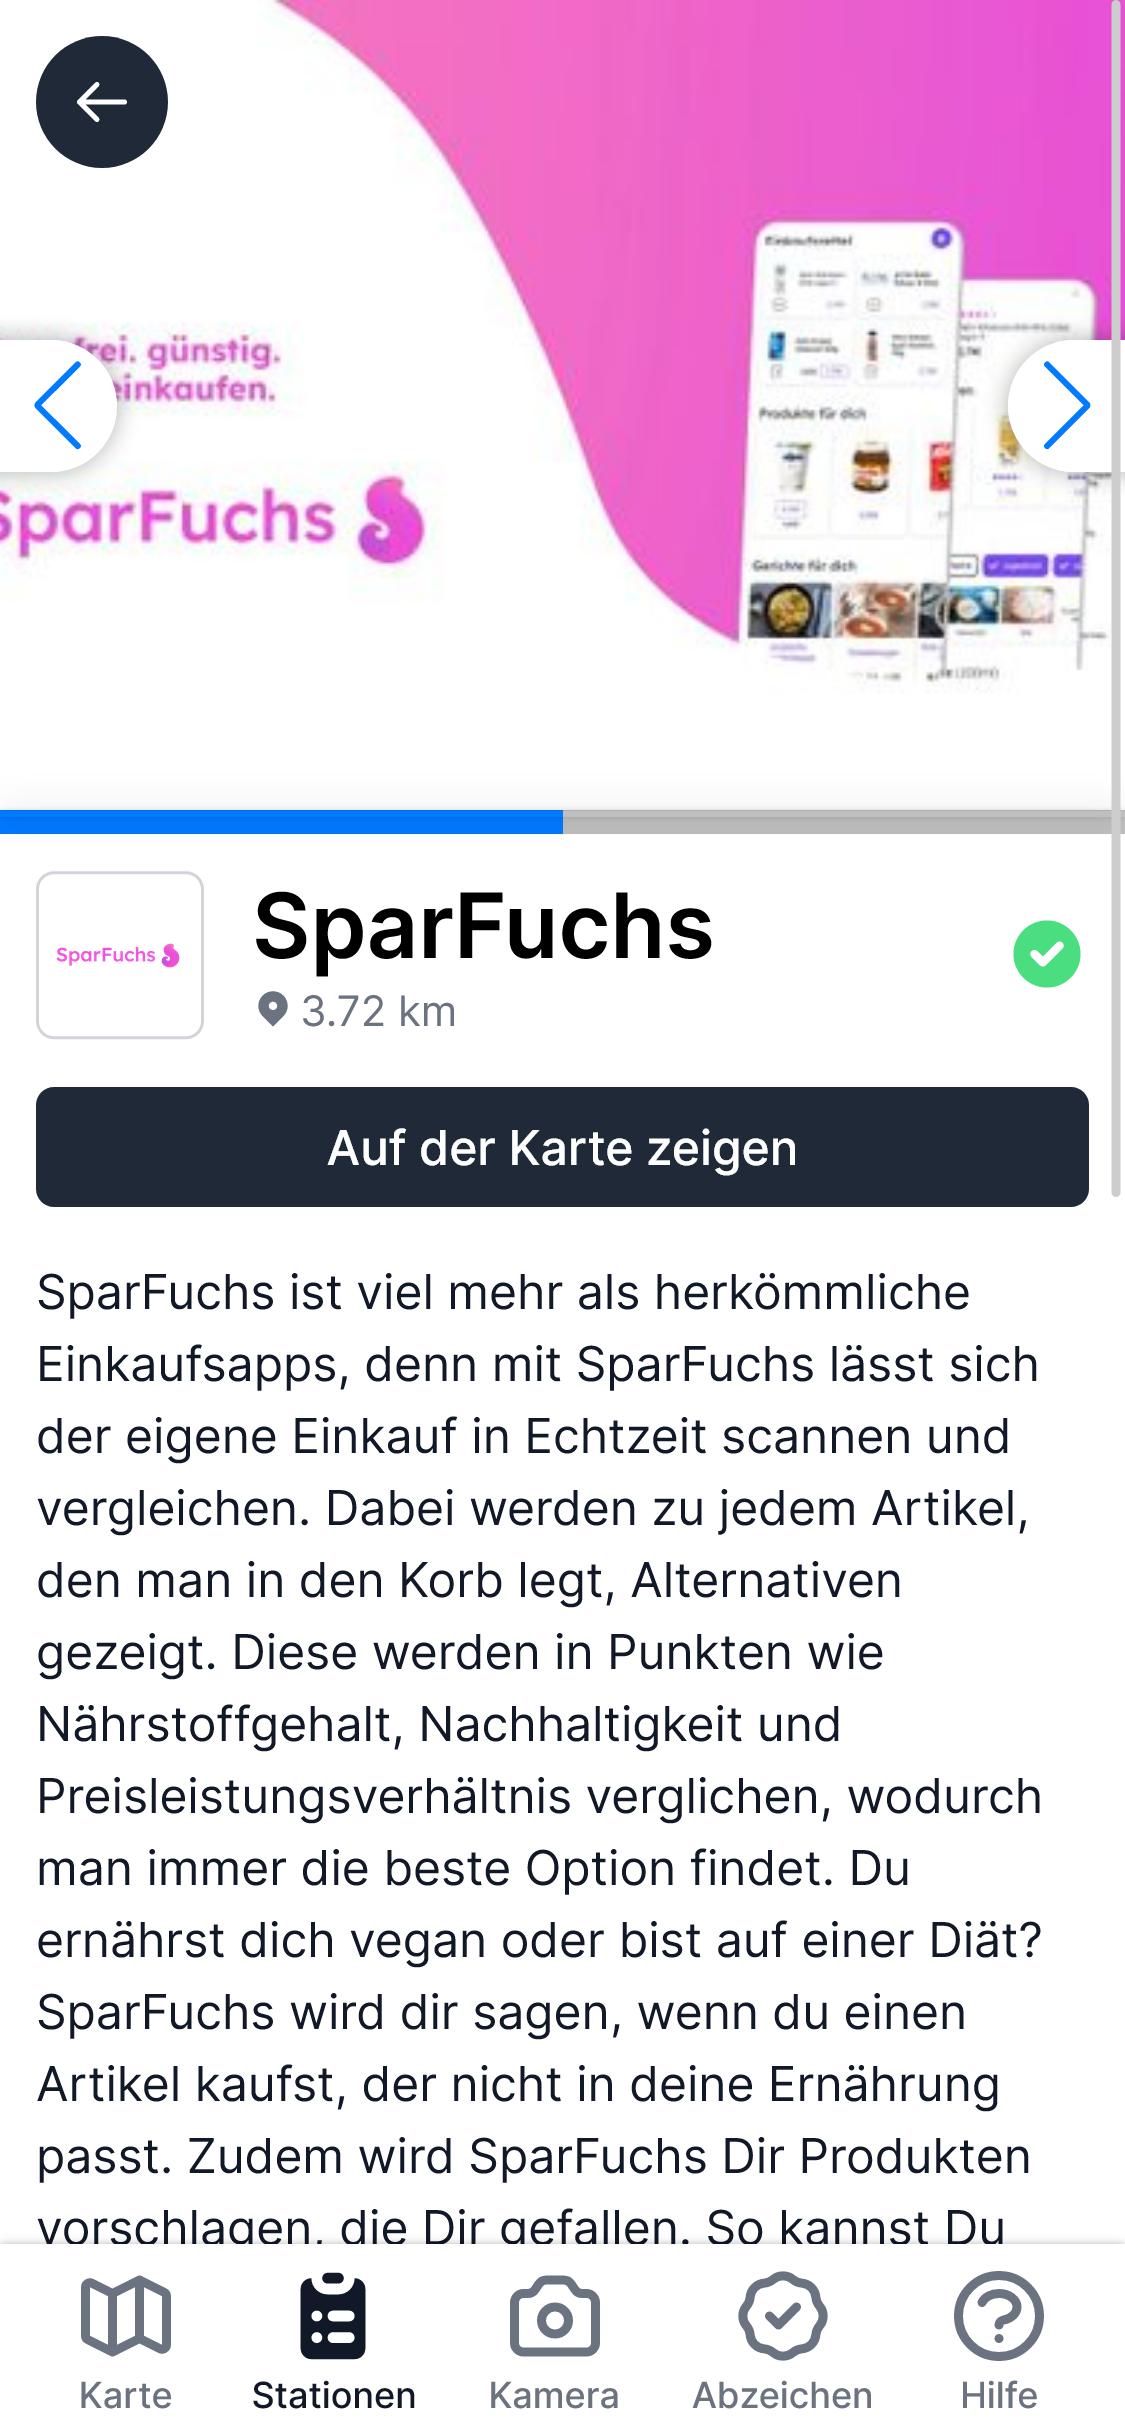
\includegraphics[width=.95\linewidth]{dialog/app/station_visible.png}
    \end{minipage}%
    \begin{minipage}{.325\textwidth}
        \centering
        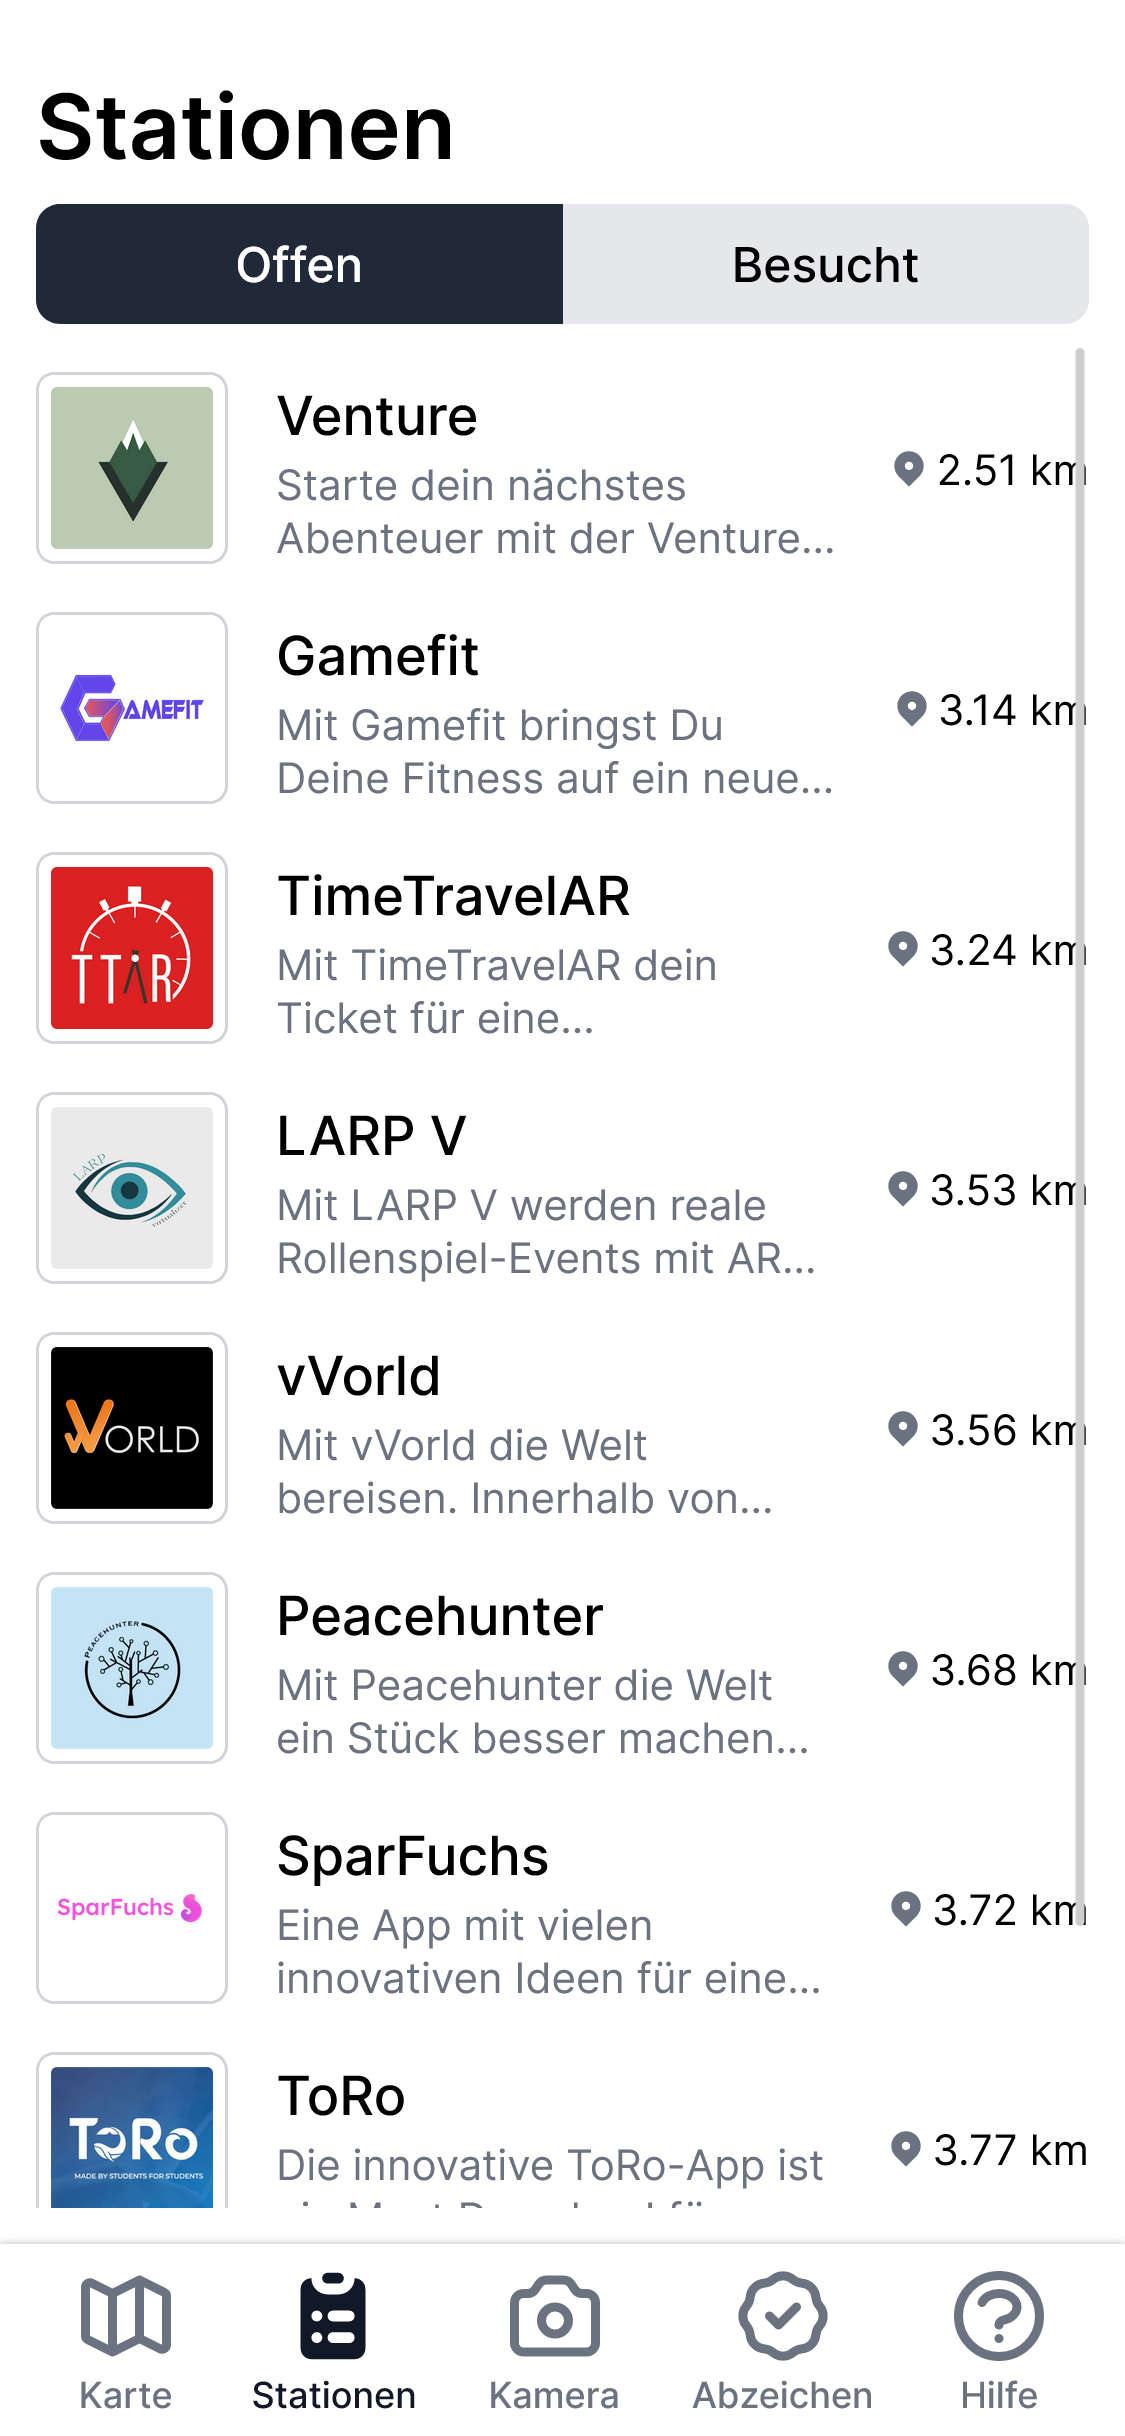
\includegraphics[width=.95\linewidth]{dialog/app/stations.png}
    \end{minipage}
    \begin{minipage}{.325\textwidth}
        \centering
        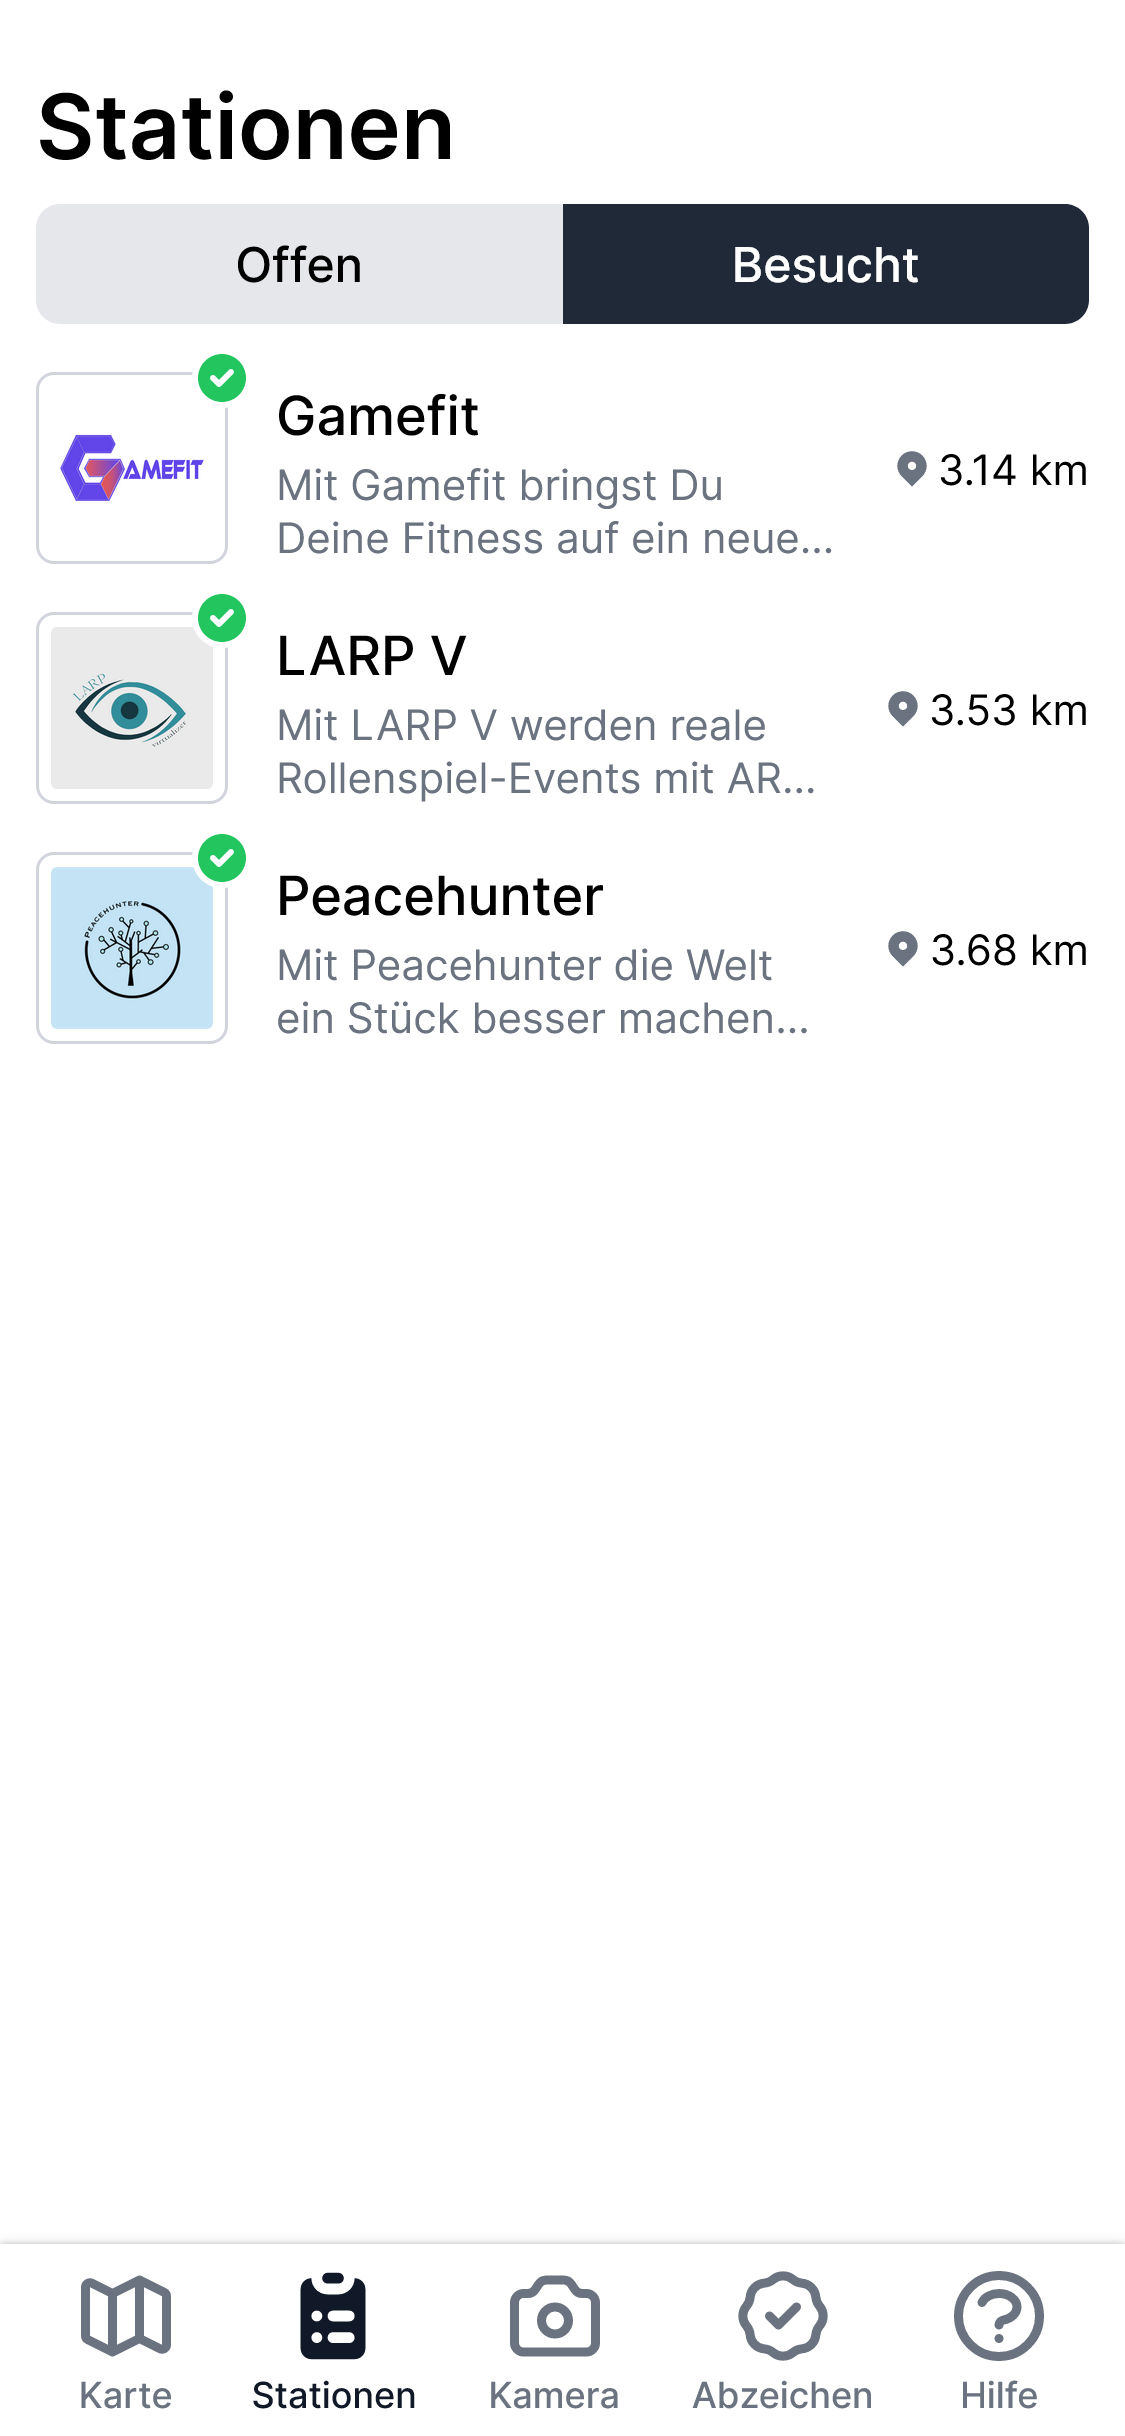
\includegraphics[width=.95\linewidth]{dialog/app/stations_visited_some.png}
    \end{minipage}
    \caption{Web-App - Stationsübersicht}
    \label{fig:dialog-t-station-visited}
\end{figure}

Nach einigen Stunden fällt Christina auf, dass sie keine unbesuchten Stationen
mehr ihrer Karte sieht (\autoref{fig:dialog-t-station-visited-all}). Als sie
zur Stationsliste wechselt, bestätigt sich, dass sie bereits alle Stationen
besucht hat. Als sie „Und die Abzeichen?“ liest, bemerkt sie jedoch, dass sie
diese völlig vergessen hat und tippt die Schaltfläche an. Bei den Abzeichen
angekommen verschafft sie sich zuerst einen Überblick, welche Abzeichen es
überhaupt gibt.

\begin{figure}[htpb]
    \centering
    \begin{minipage}{.325\textwidth}
        \centering
        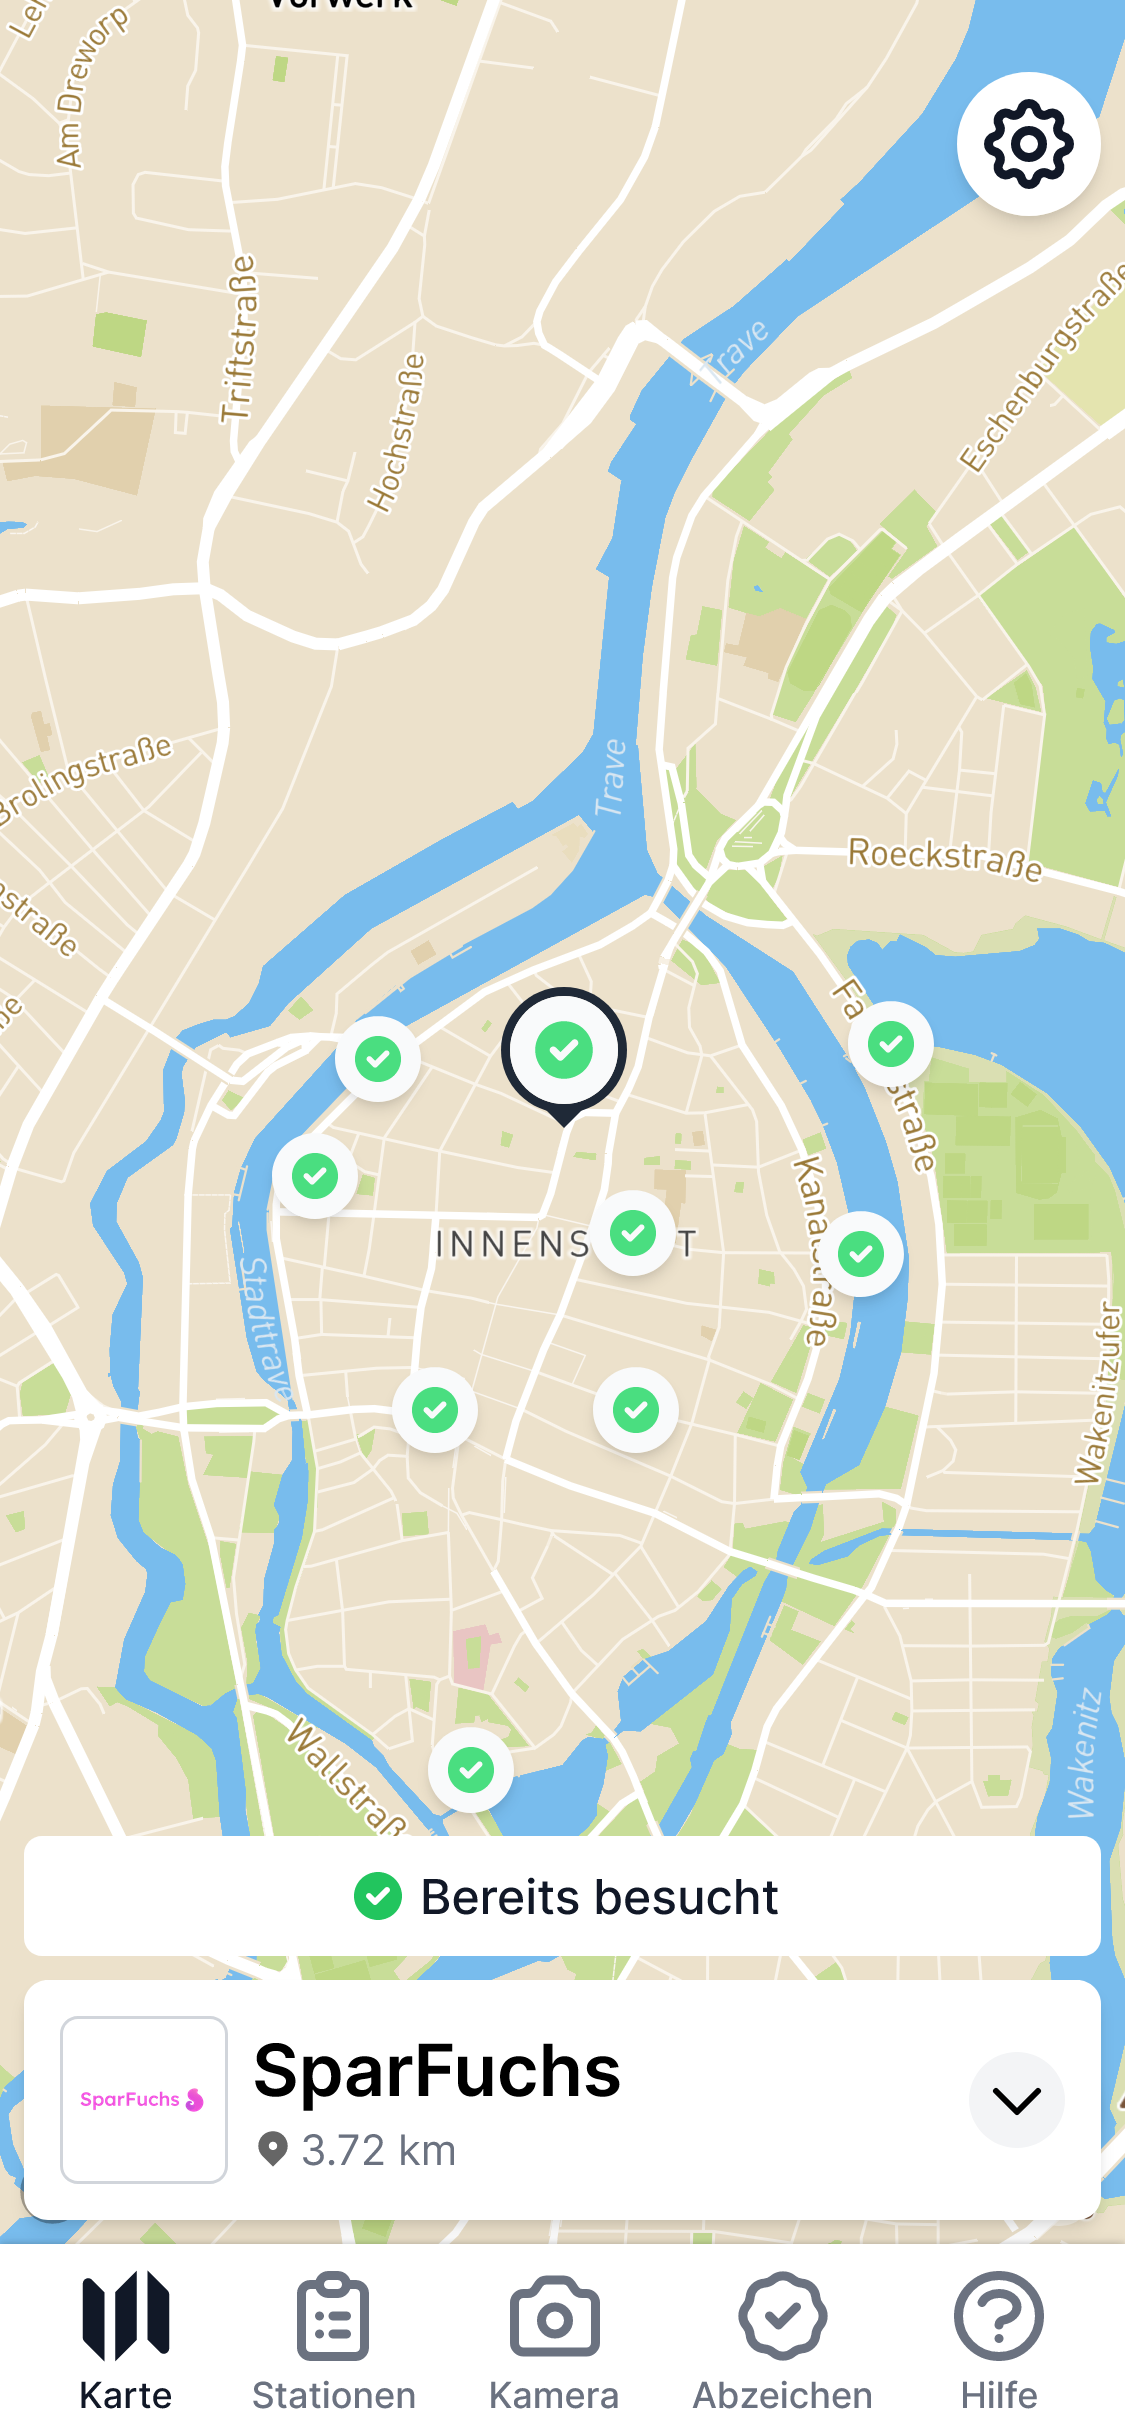
\includegraphics[width=.95\linewidth]{dialog/app/map_visited.png}
    \end{minipage}%
    \begin{minipage}{.325\textwidth}
        \centering
        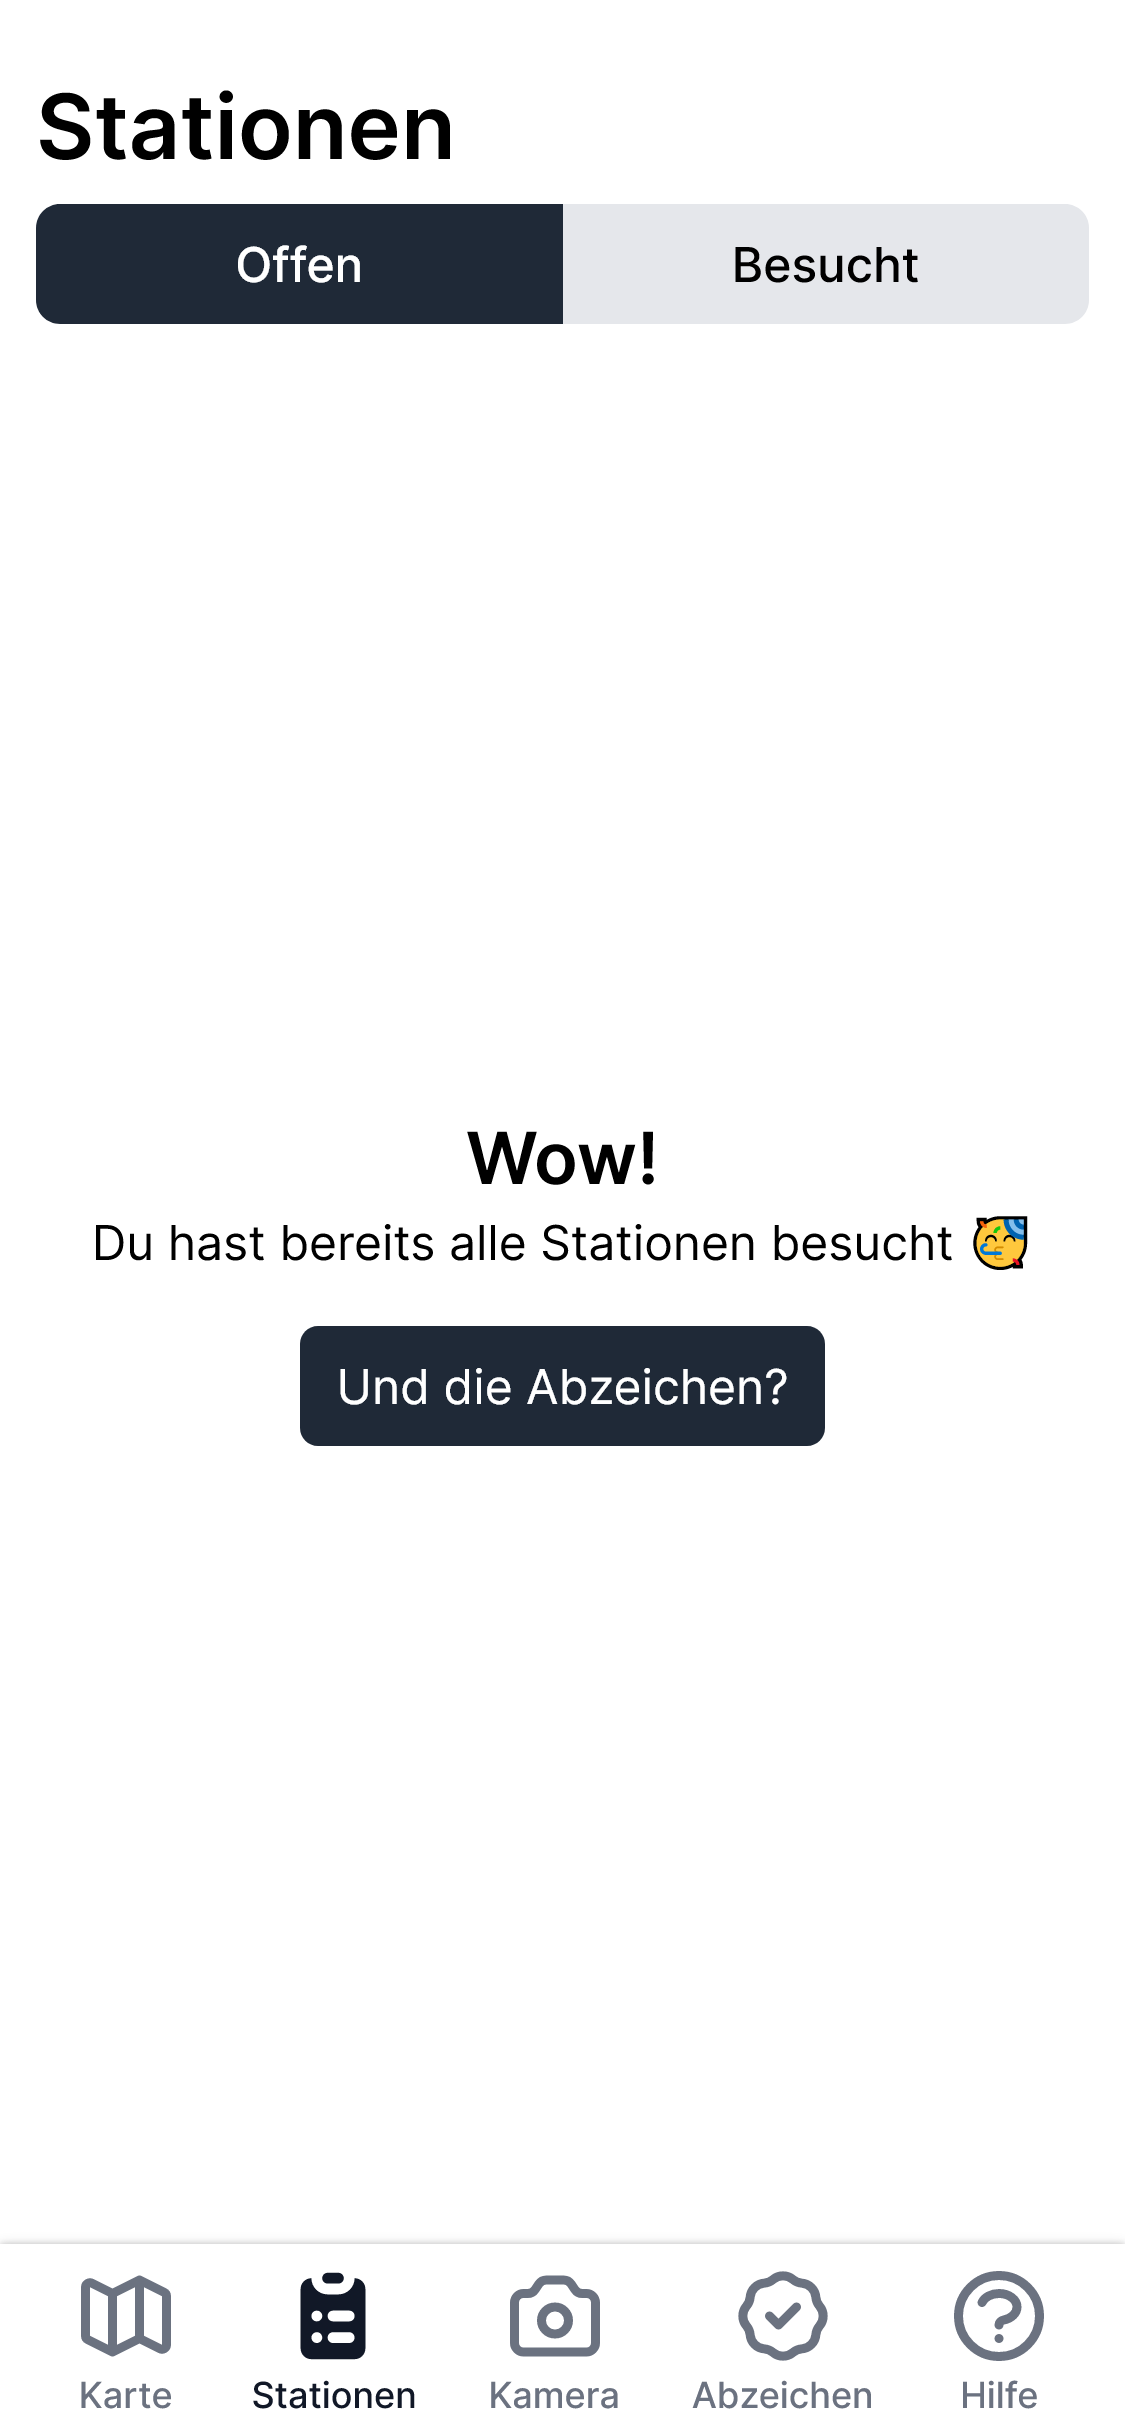
\includegraphics[width=.95\linewidth]{dialog/app/stations_visited_all.png}
    \end{minipage}
    \begin{minipage}{.325\textwidth}
        \centering
        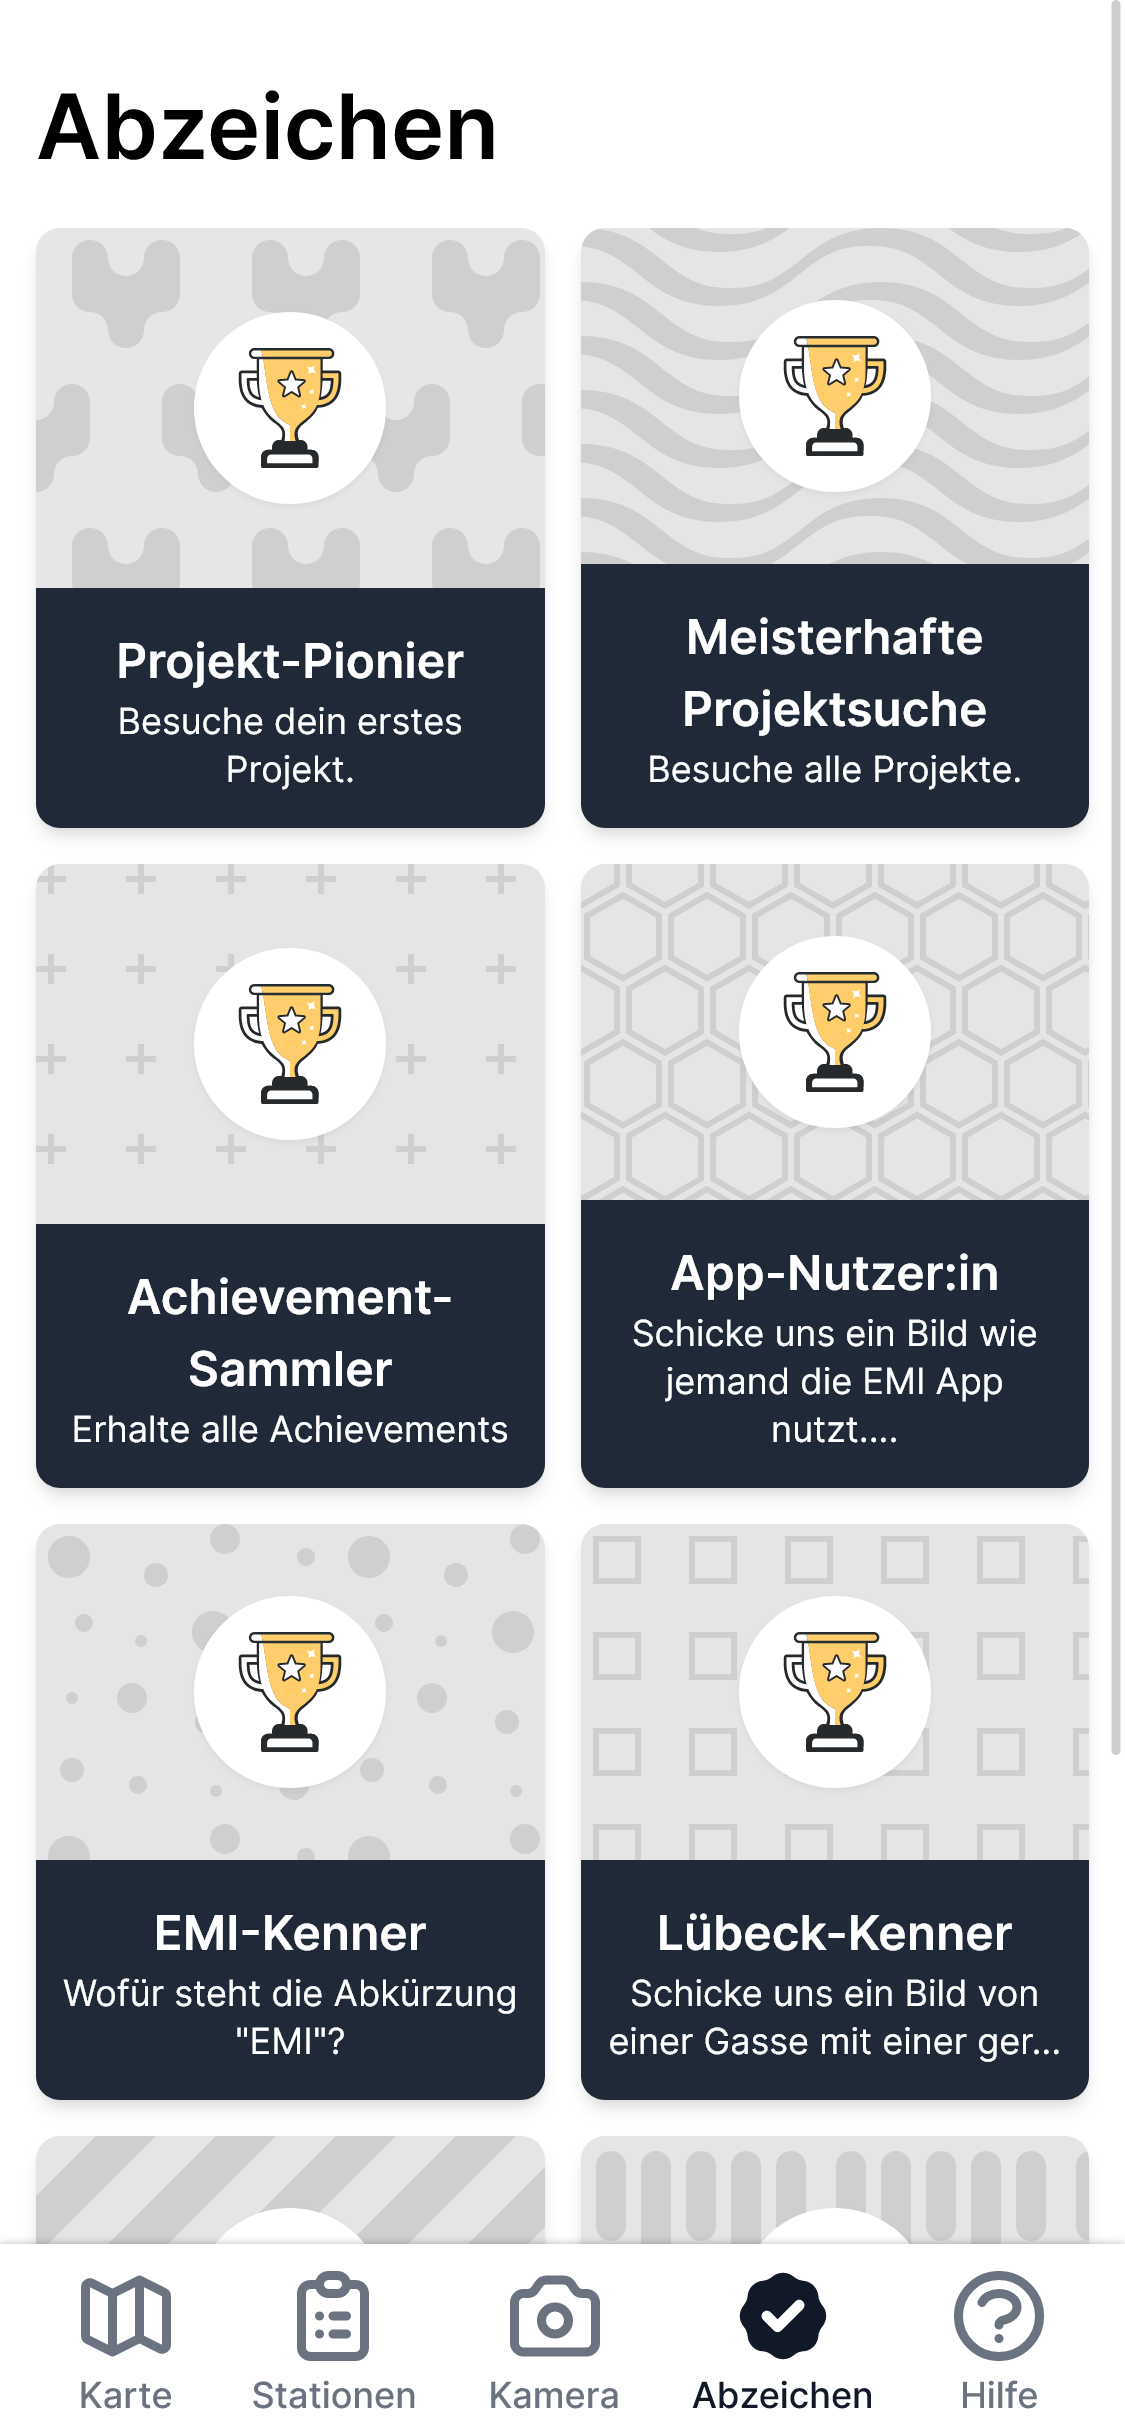
\includegraphics[width=.95\linewidth]{dialog/app/achievements.png}
    \end{minipage}
    \caption{Web-App - Alle Stationen besucht}
    \label{fig:dialog-t-station-visited-all}
\end{figure}

Schließlich bleibt Christina bei dem Abzeichen „Prominenz“ hängen und tippt
dieses an (\autoref{fig:dialog-t-achievement}). Im Abzeichen wird Christina
nach dem prominenten Kumpel von Prof. Schrader gefragt. Das weiß sie natürlich
sofort und tippt eifrig „Hank“ in das Abgabefeld ein. Nachdem Christina ihre
Antwort eingereicht hat, fällt ihr das gelbe Uhren-Icon auf. Anscheinend muss
sie warten, während die Antwort überprüft wird.

\begin{figure}[htpb]
    \centering
    \begin{minipage}{.325\textwidth}
        \centering
        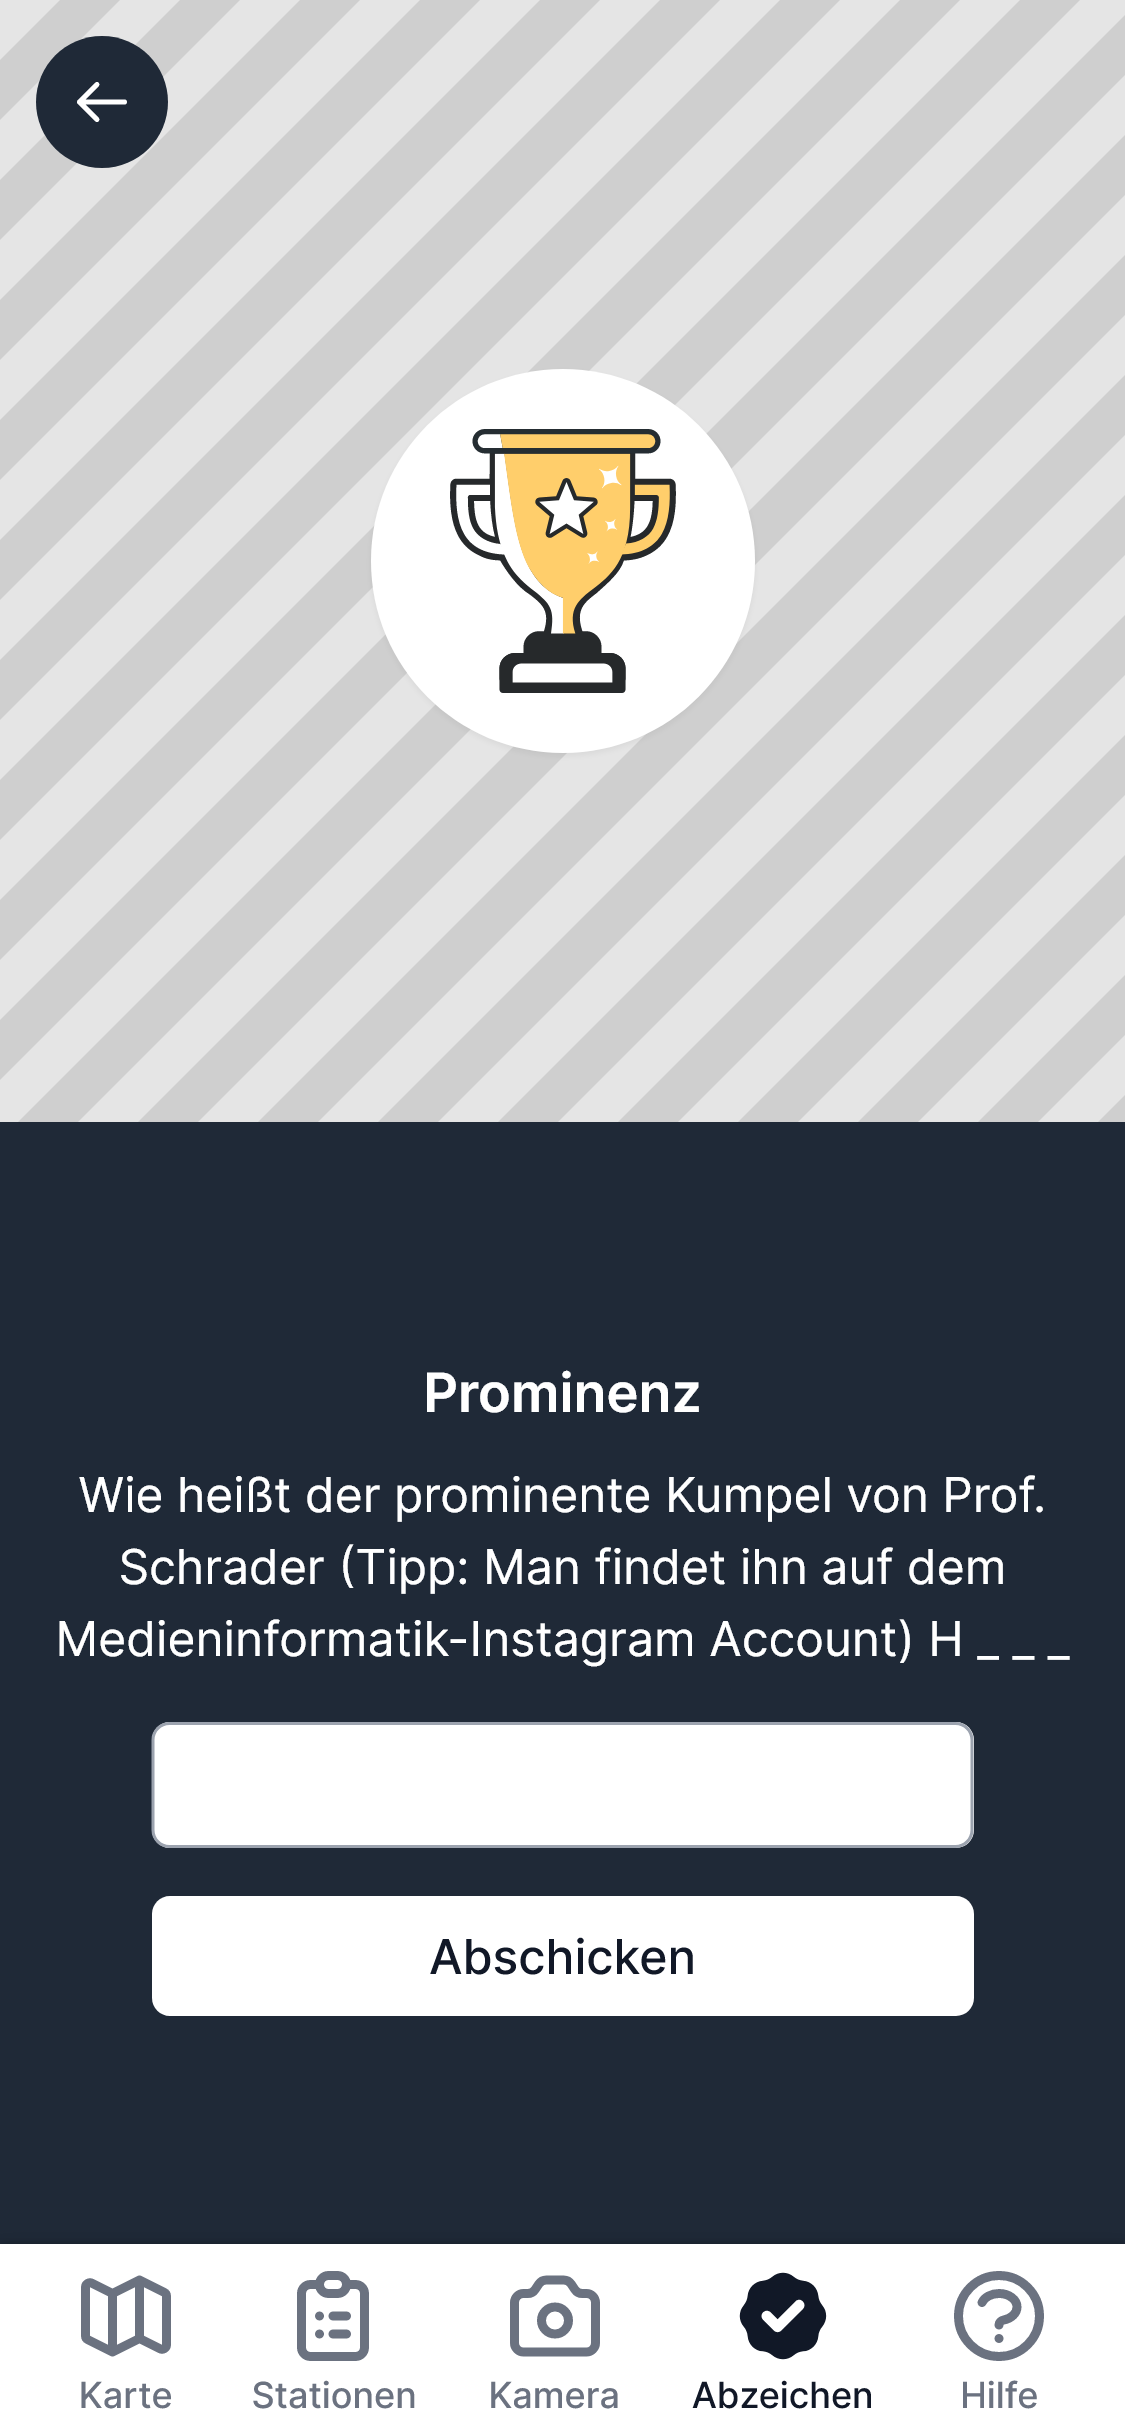
\includegraphics[width=.95\linewidth]{dialog/app/achievement_text.png}
    \end{minipage}%
    \begin{minipage}{.325\textwidth}
        \centering
        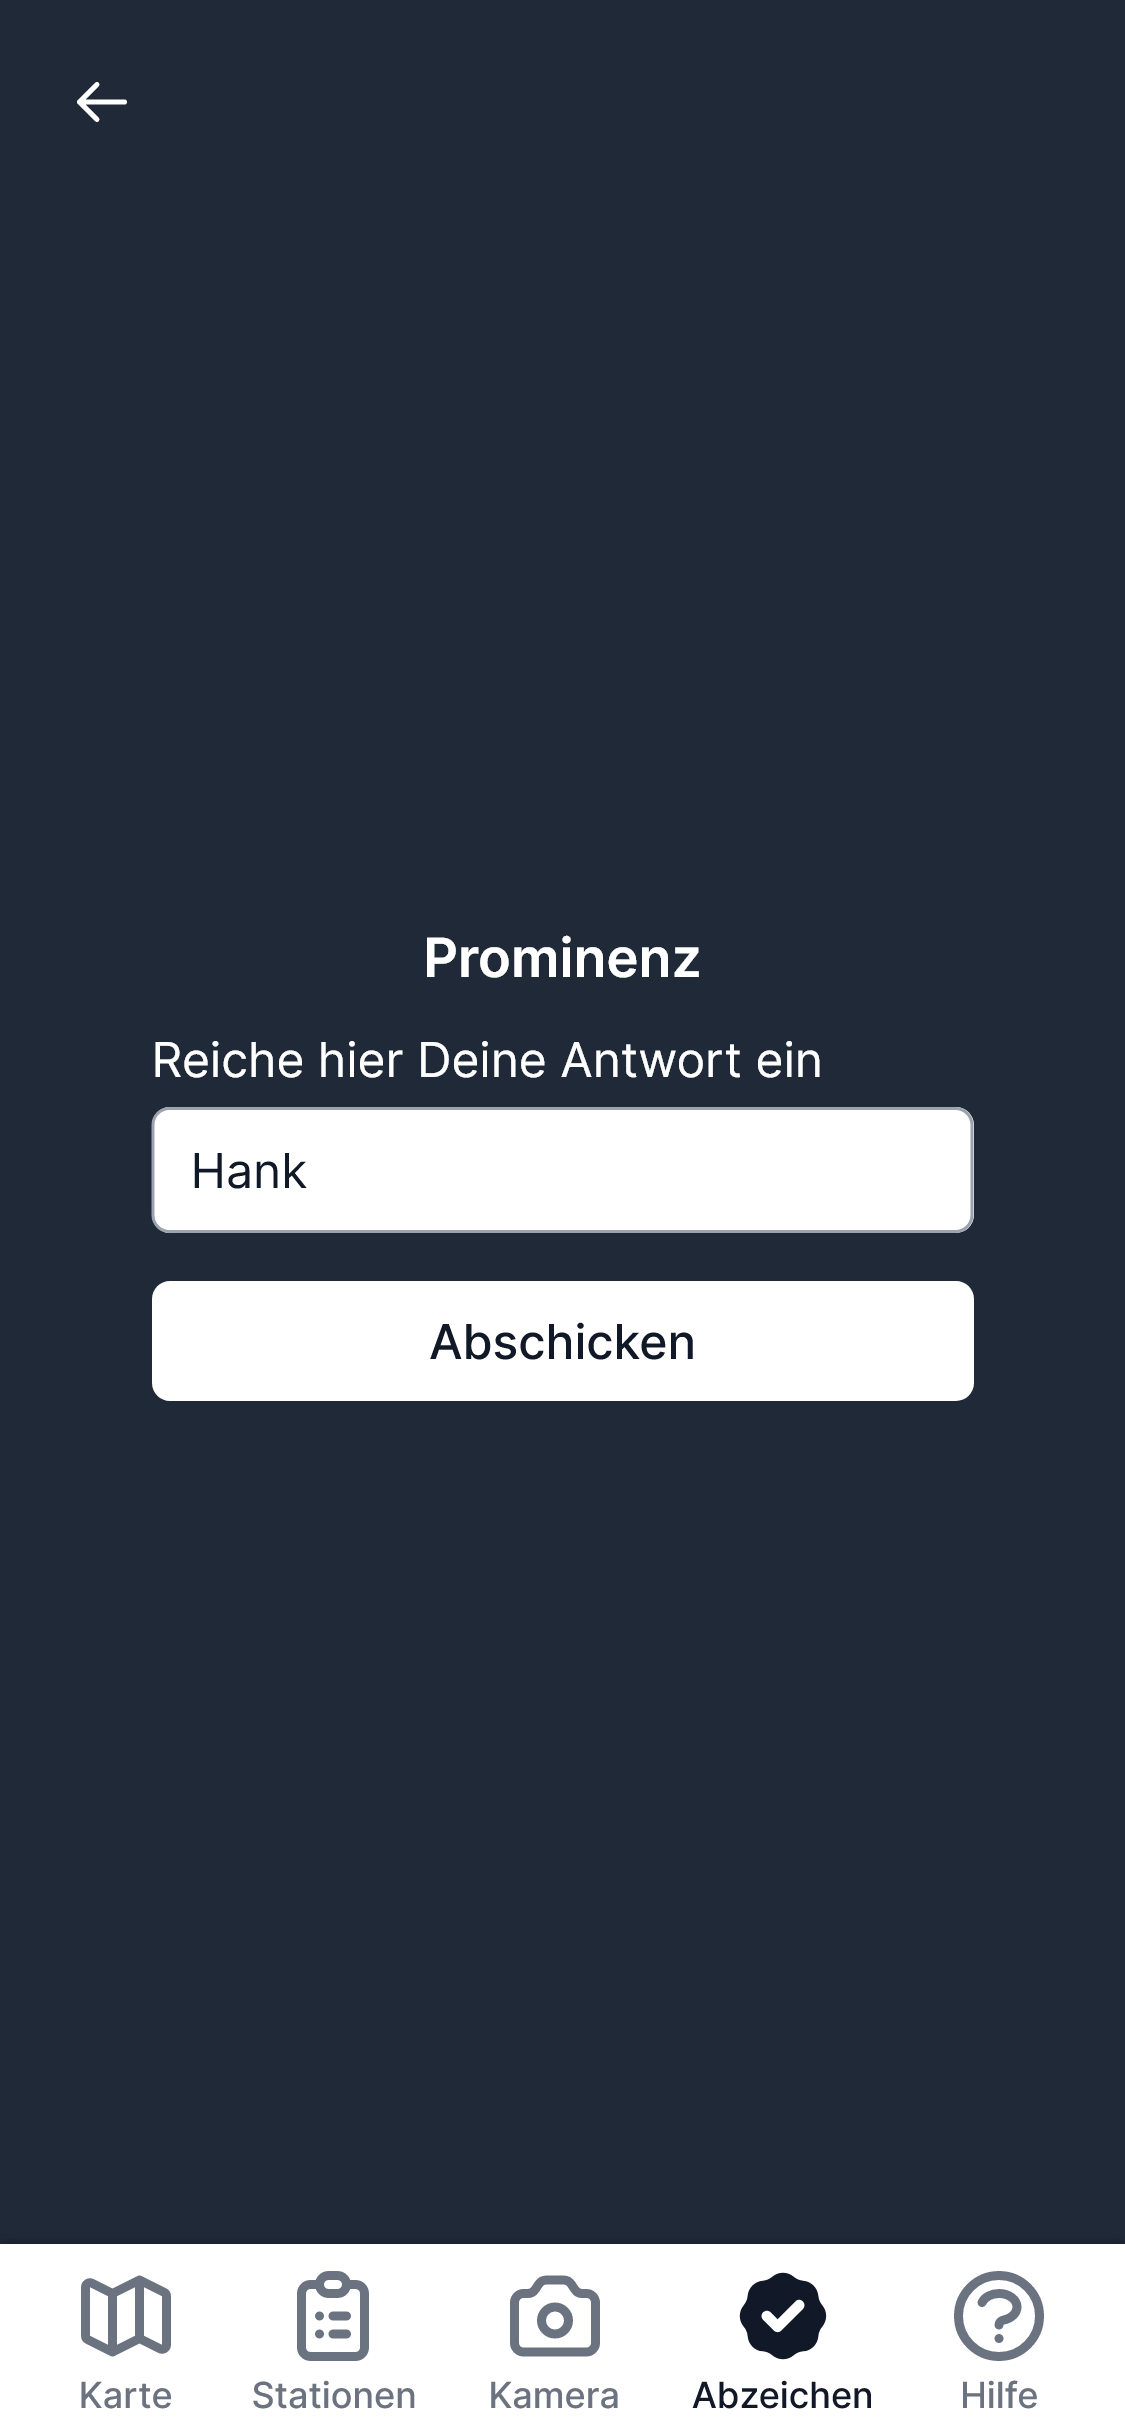
\includegraphics[width=.95\linewidth]{dialog/app/achievement_text_open.png}
    \end{minipage}
    \begin{minipage}{.325\textwidth}
        \centering
        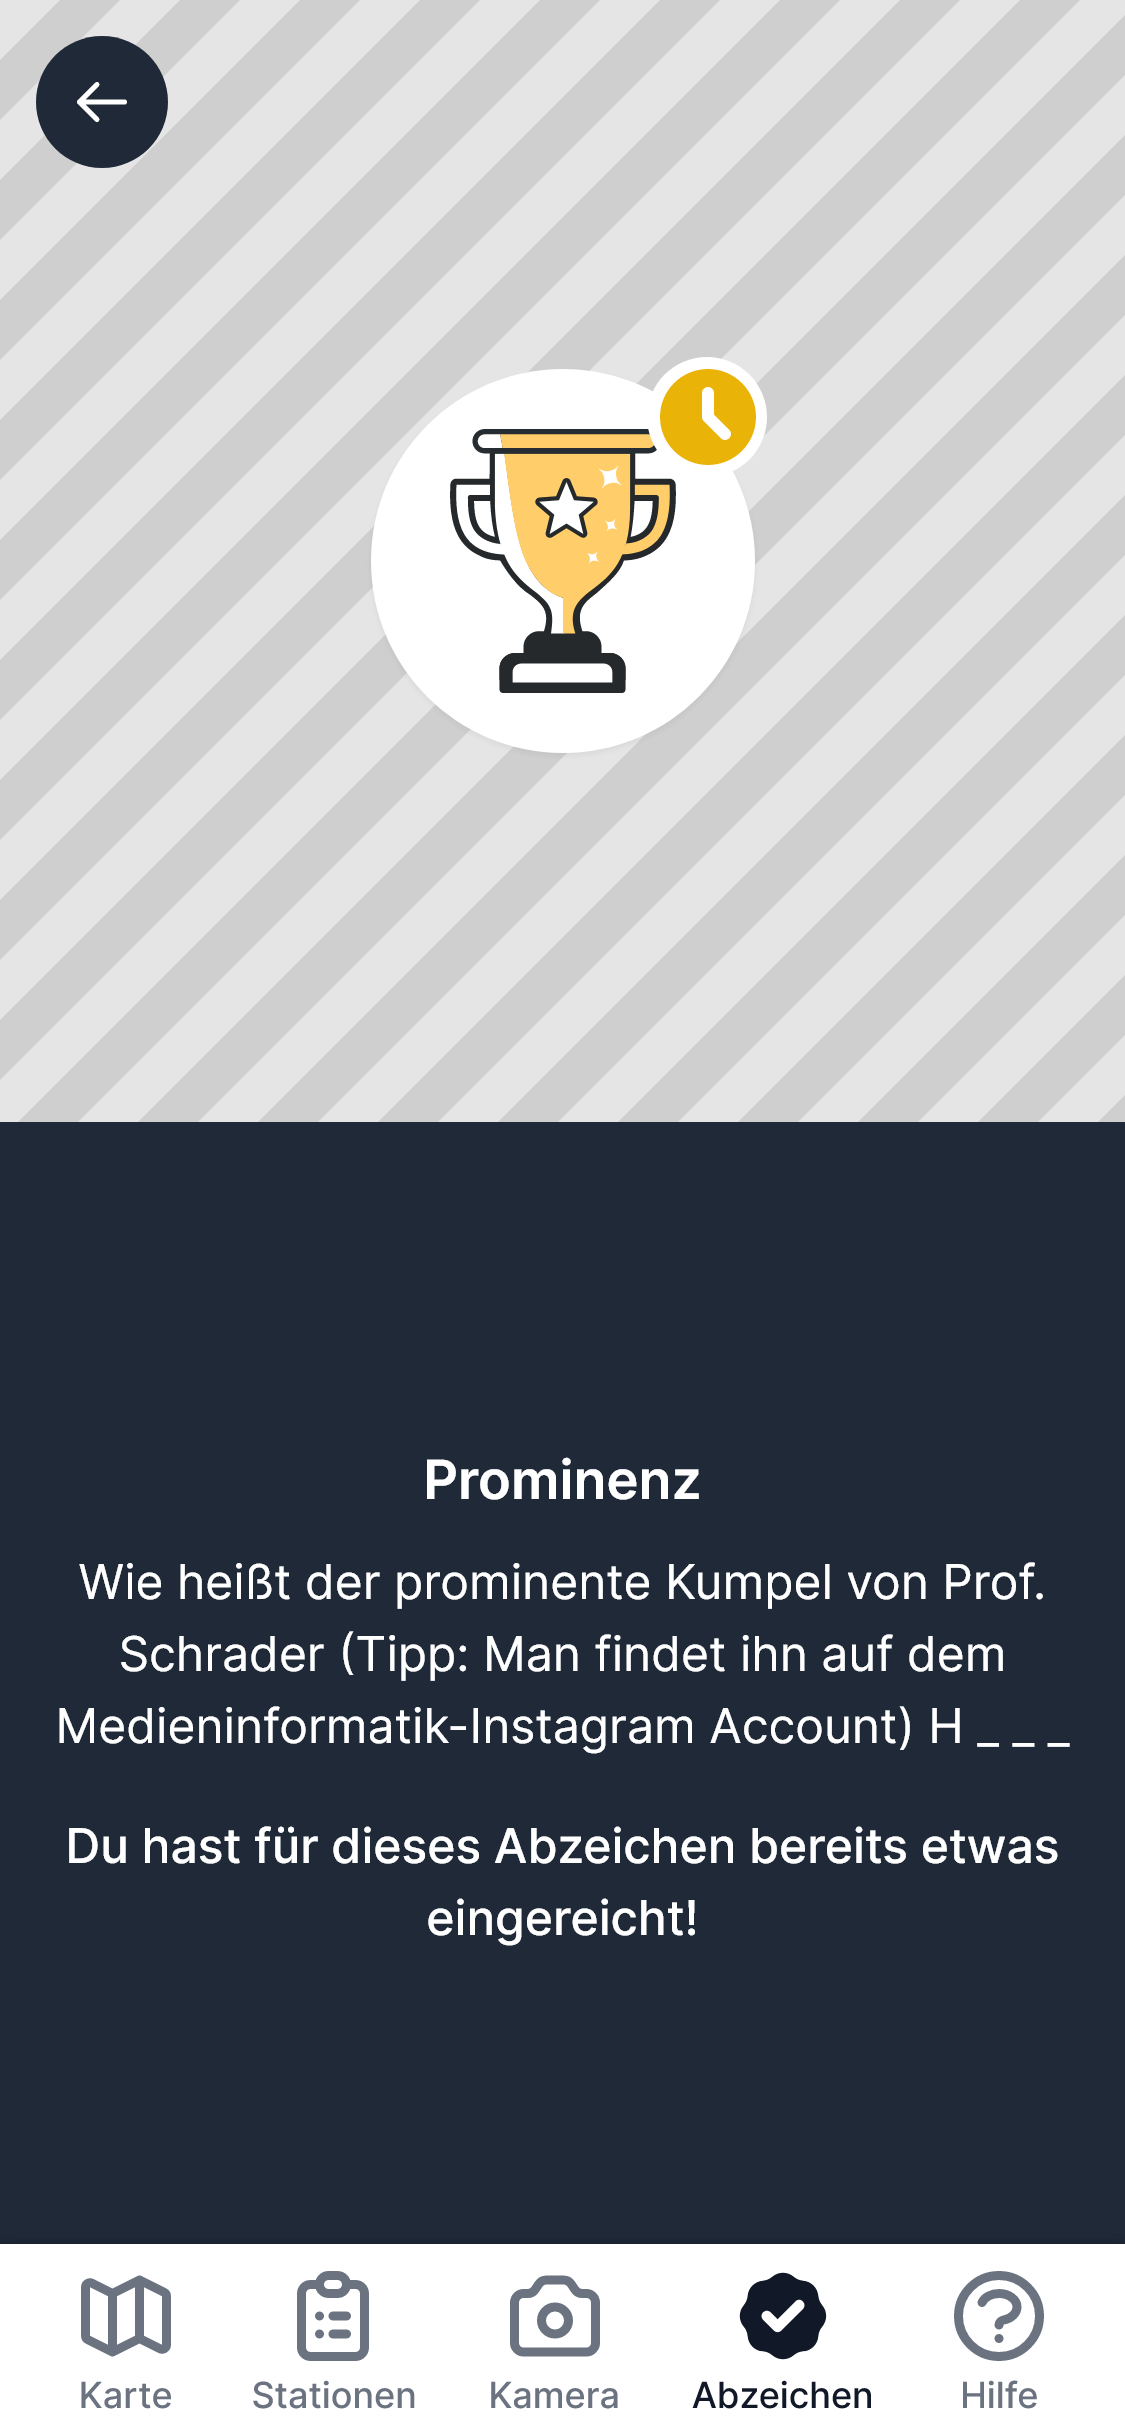
\includegraphics[width=.95\linewidth]{dialog/app/achievement_submitted.png}
    \end{minipage}
    \caption{Web-App - Textabzeichen}
    \label{fig:dialog-t-achievement}
\end{figure}

Im selben Moment ist Sven auf dem Dashboard und wechselt zu den
Abzeicheneinreichungen aus \autoref{fig:dialog-v-achievements}, um zu sehen, ob
jemand bereits etwas eingereicht hat. Dabei fällt Sven Christinas Einreichung
auf, welche er schnell antippt. Hiermit wird Sven zur Einreichung aus
\autoref{fig:dialog-v-achievement-submission} weitergeleitet, welche er auf ihre
Richtigkeit überprüft. Christina hat richtig geantwortet, also klickt Sven auf
die „Akzeptieren“ Schaltfläche.

\begin{figure}[htpb]
    \centering
    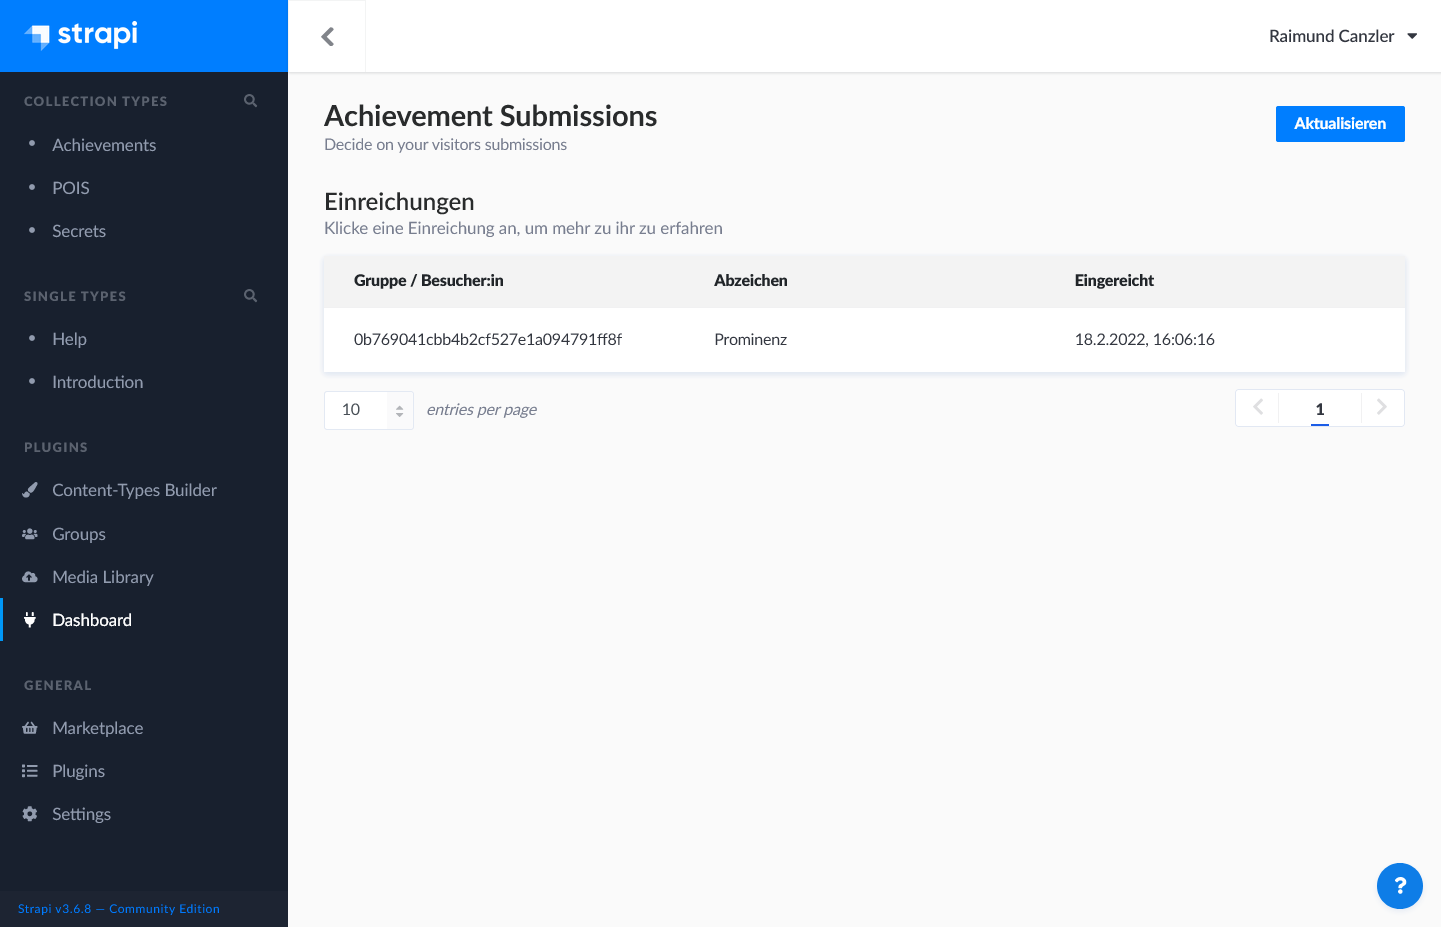
\includegraphics[width=\linewidth]{dialog/dashboard/achievement.png}
    \caption{Dashboard - Übersicht der Abzeicheneinreichungen}
    \label{fig:dialog-v-achievements}
\end{figure}

\begin{figure}[htpb]
    \centering
    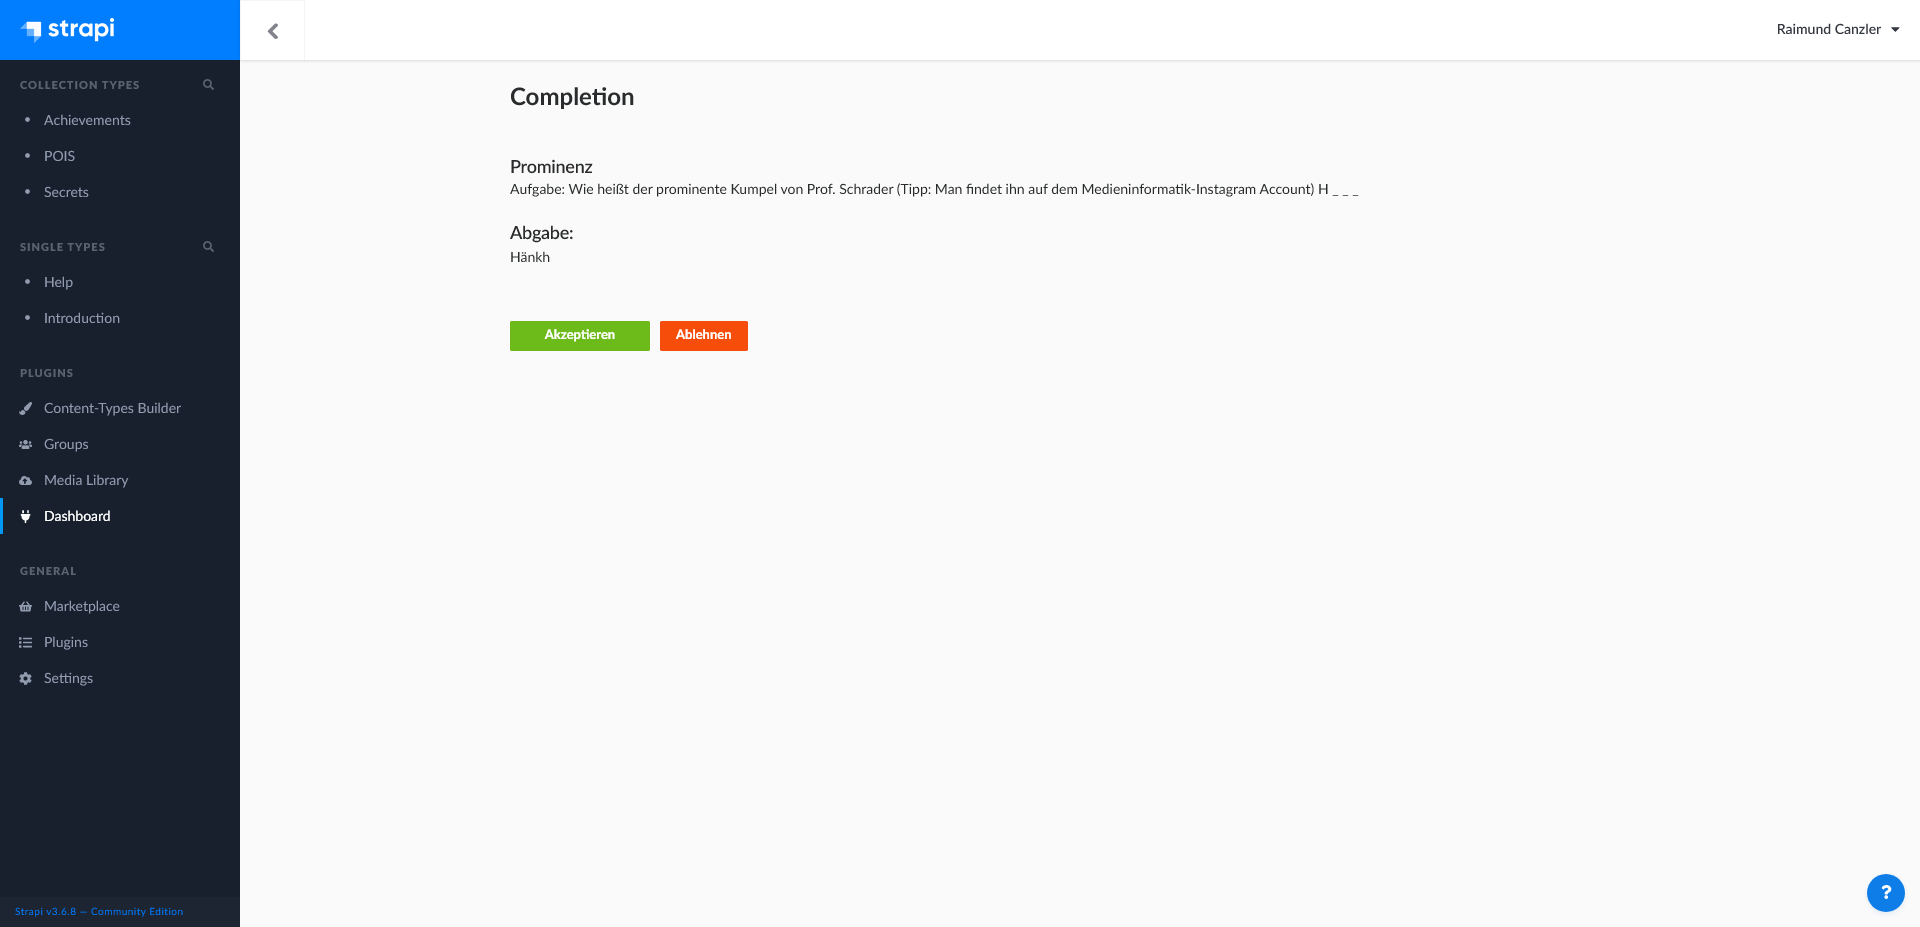
\includegraphics[width=\linewidth]{dialog/dashboard/achievement_submission.png}
    \caption{Dashboard - Bewertung der Abzeicheneinreichungen}
    \label{fig:dialog-v-achievement-submission}
\end{figure}


Während Christina sich die anderen Abzeichen angeschaut hat, wird ihr plötzlich
eine Benachrichtigung angezeigt (\autoref{fig:dialog-t-achievement-accepted}). Vor Freude tippt sie auf die
Benachrichtigung und sieht, dass ihre Einreichung richtig war.

\begin{figure}[htpb]
    \centering
    \begin{minipage}{.5\textwidth}
        \centering
        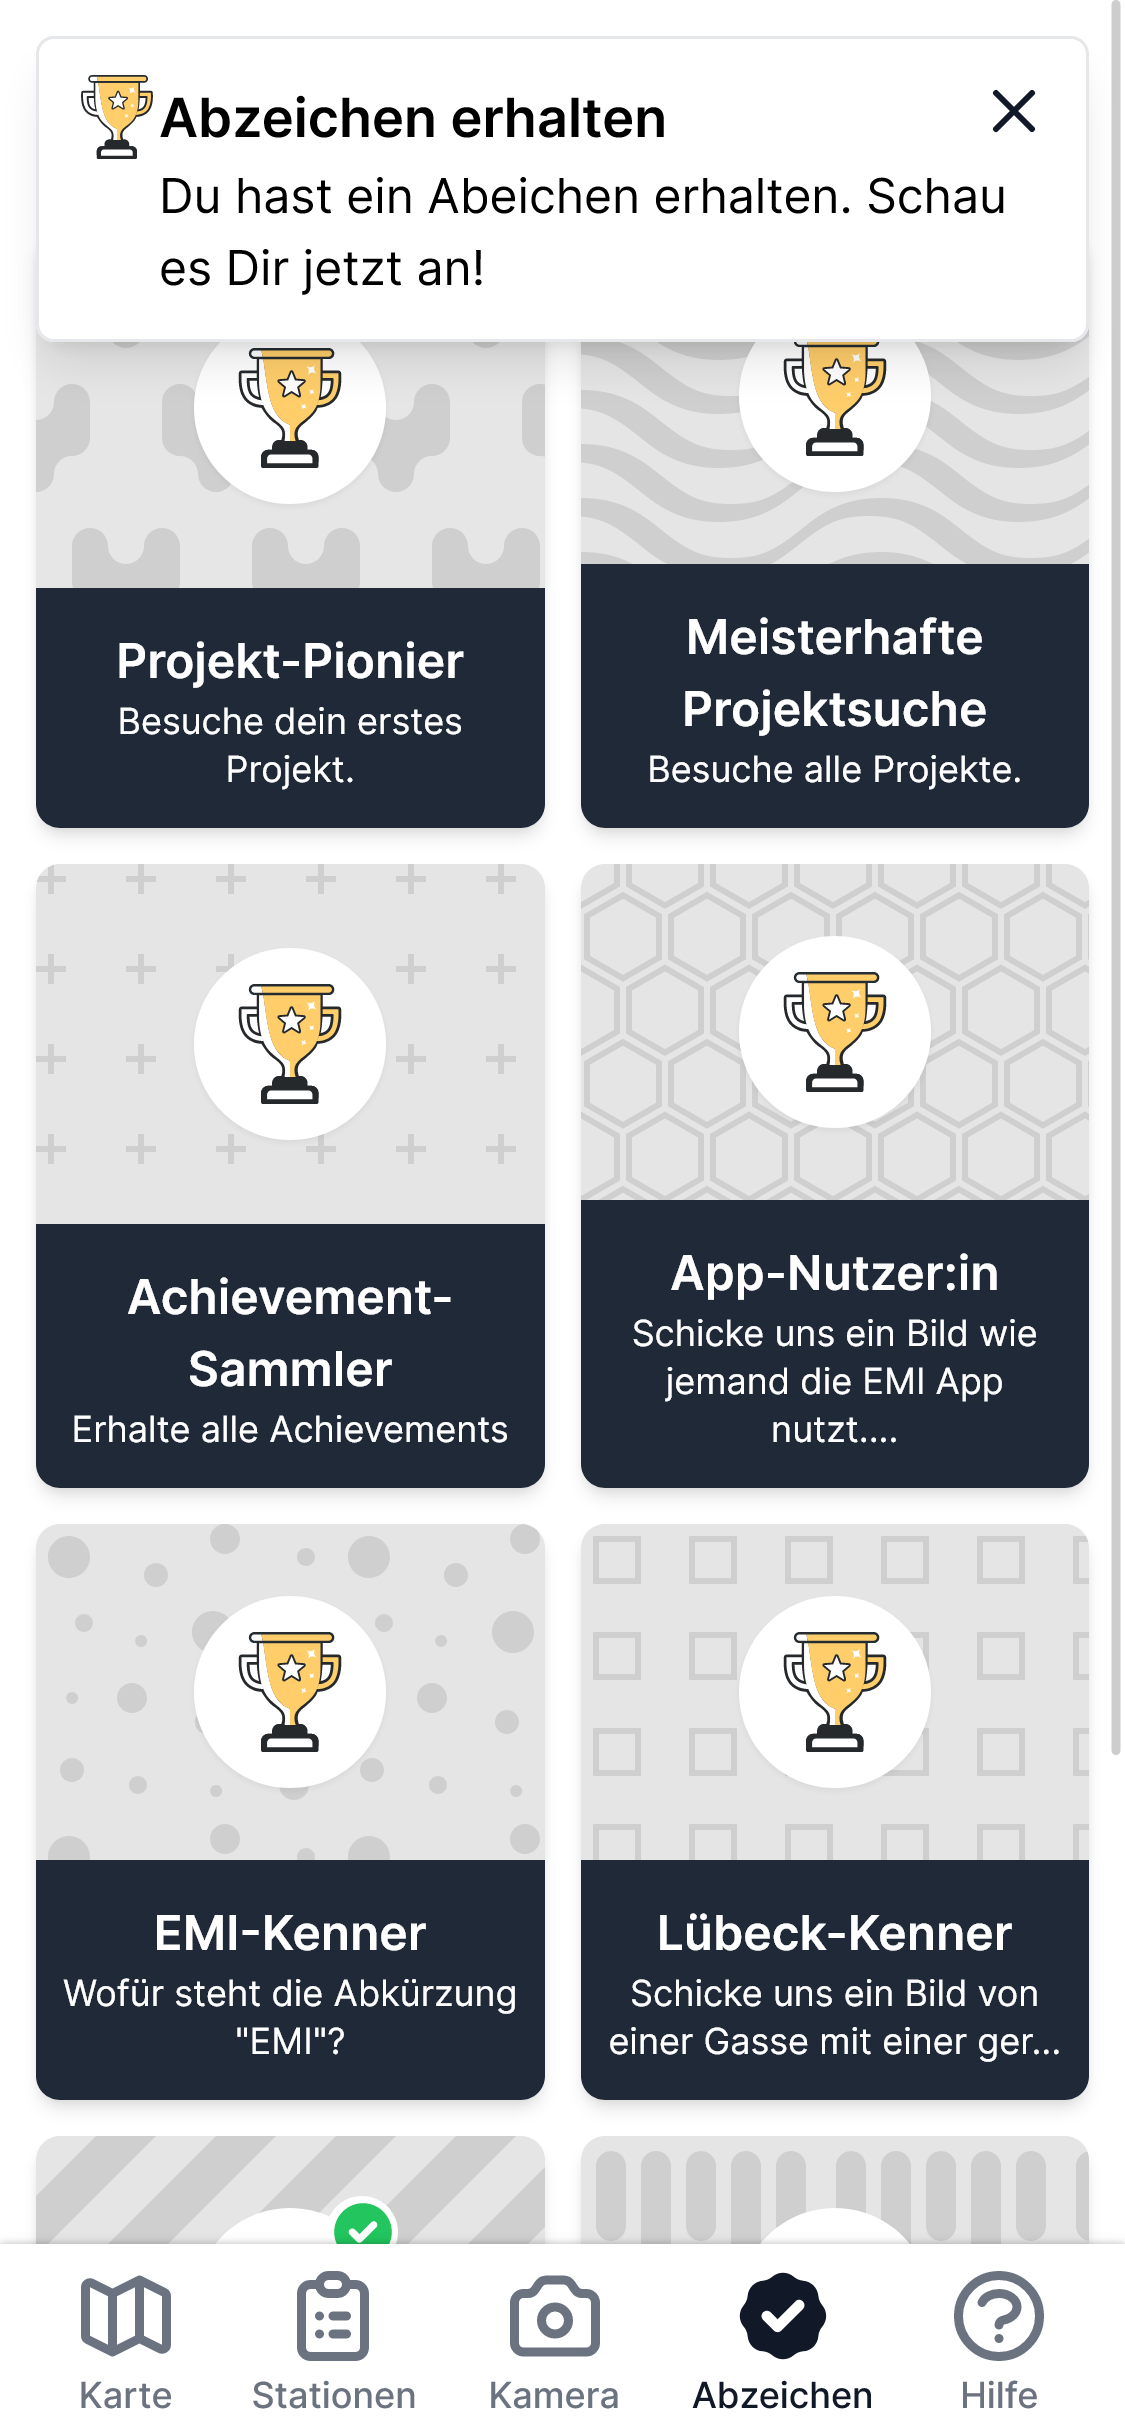
\includegraphics[width=.6\linewidth]{dialog/app/achievement_notification.png}
    \end{minipage}%
    \begin{minipage}{.5\textwidth}
        \centering
        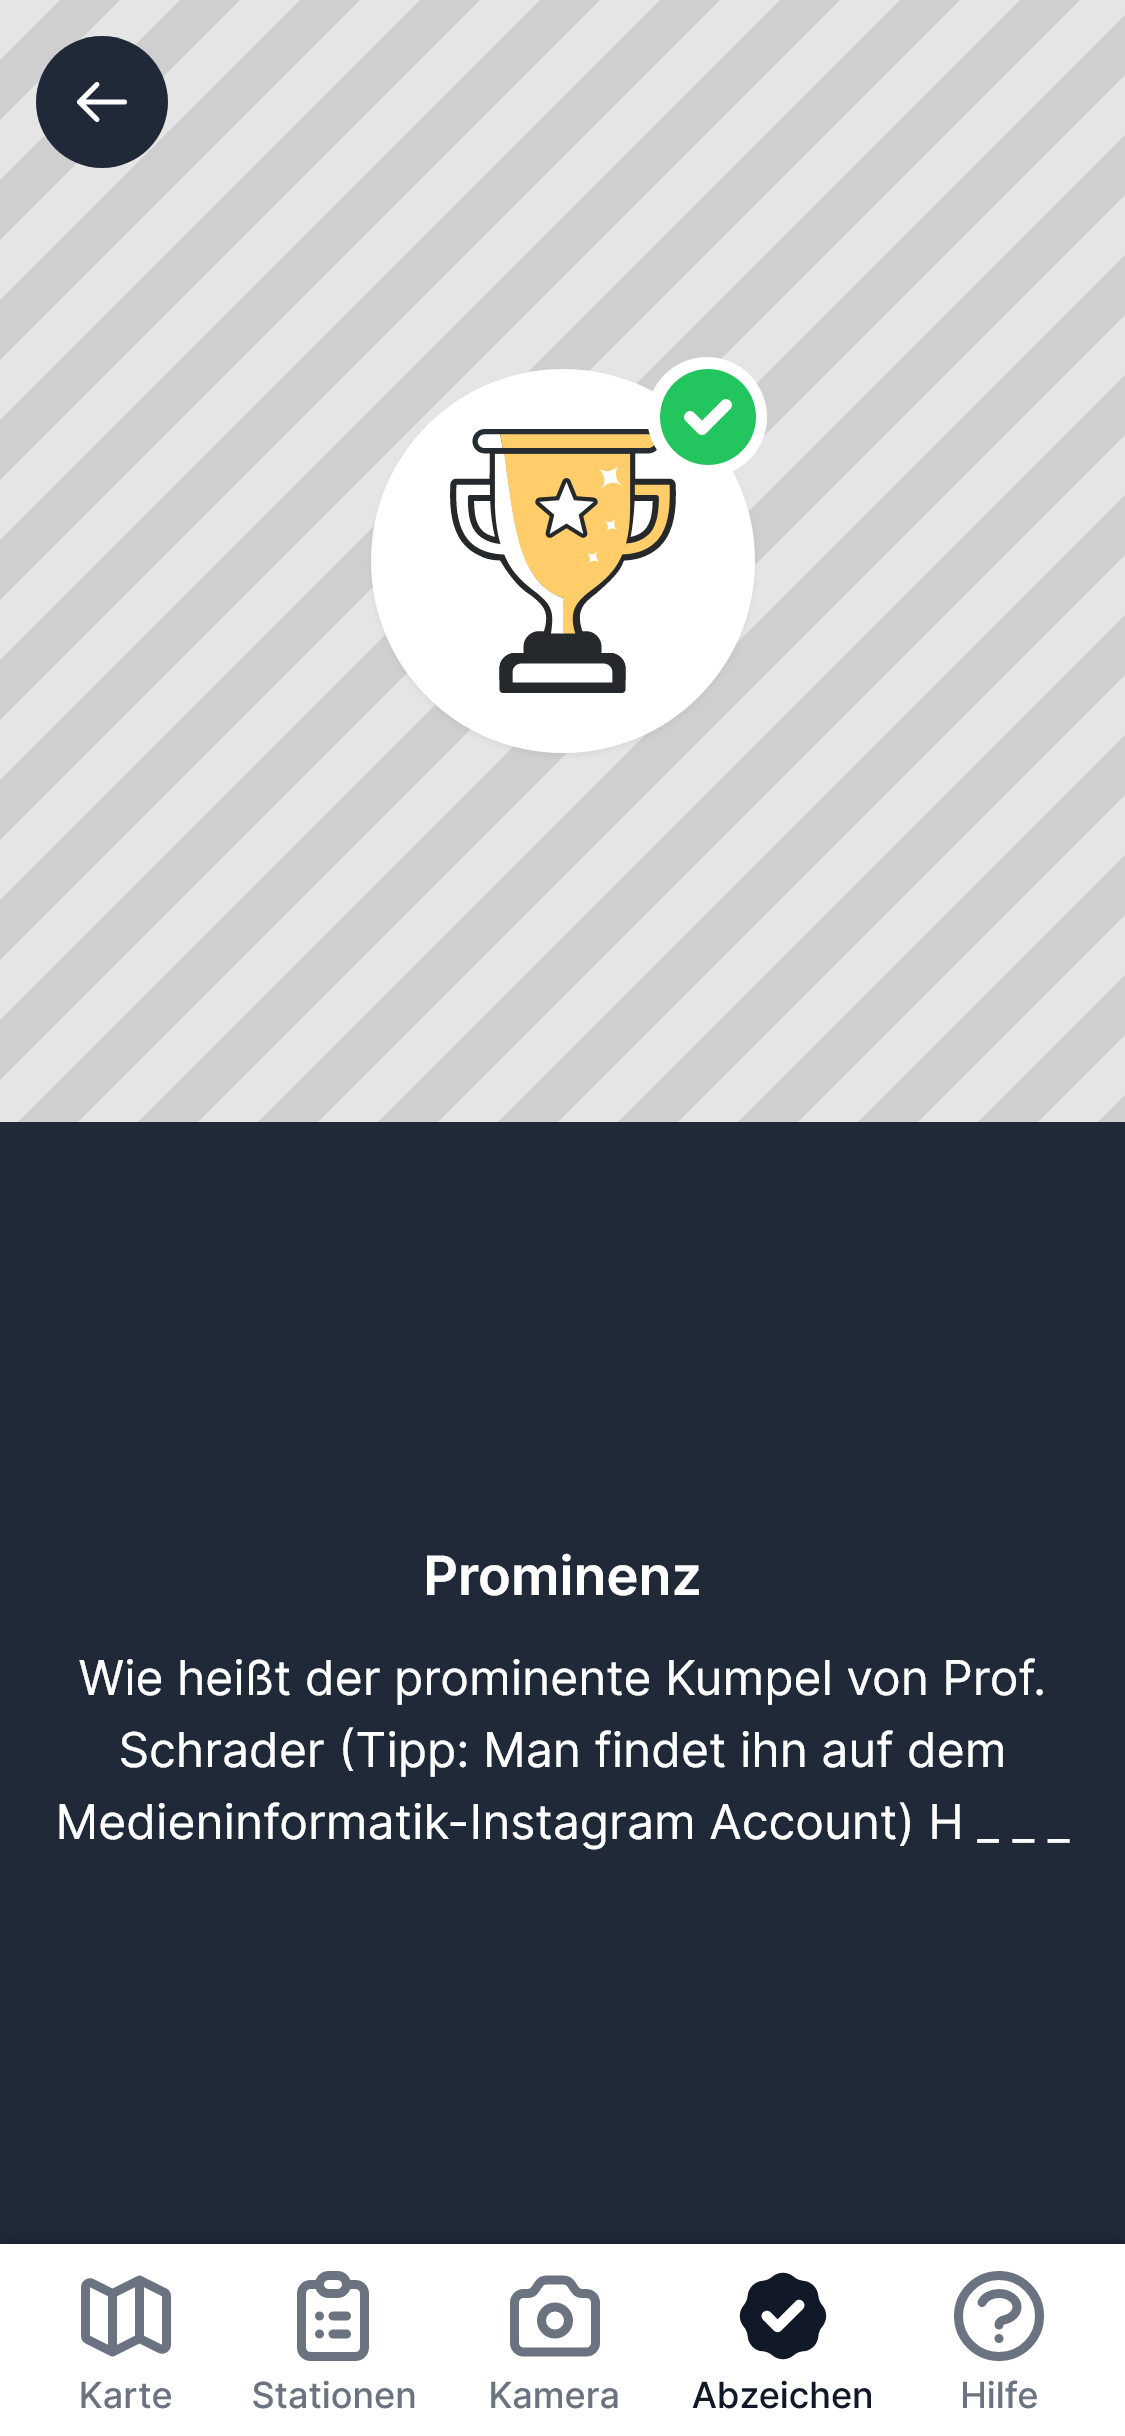
\includegraphics[width=.6\linewidth]{dialog/app/achievement_text_done.png}
    \end{minipage}
    \caption{Web-App - Abgeschlossenes Abzeichen}
    \label{fig:dialog-t-achievement-accepted}
\end{figure}

Währenddessen ist Sven damit beschäftigt, noch schnell eine Ankündigung an alle
Teilnehmenden zu schicken. Dafür füllt er die benötigten Felder auf der
Benachrichtigungsseite aus (\autoref{fig:dialog-v-notifications}) und schickt
diese ab.

Christina, welche nach wie vor durch die Stadt spaziert, fällt diese Nachricht
direkt auf. Auch wenn Christina wundert, was dieser „EMI“ sein soll, begibt sie
sich auf die Suche und geht weiter durch die Stadt.

\begin{figure}[htpb]
    \centering
    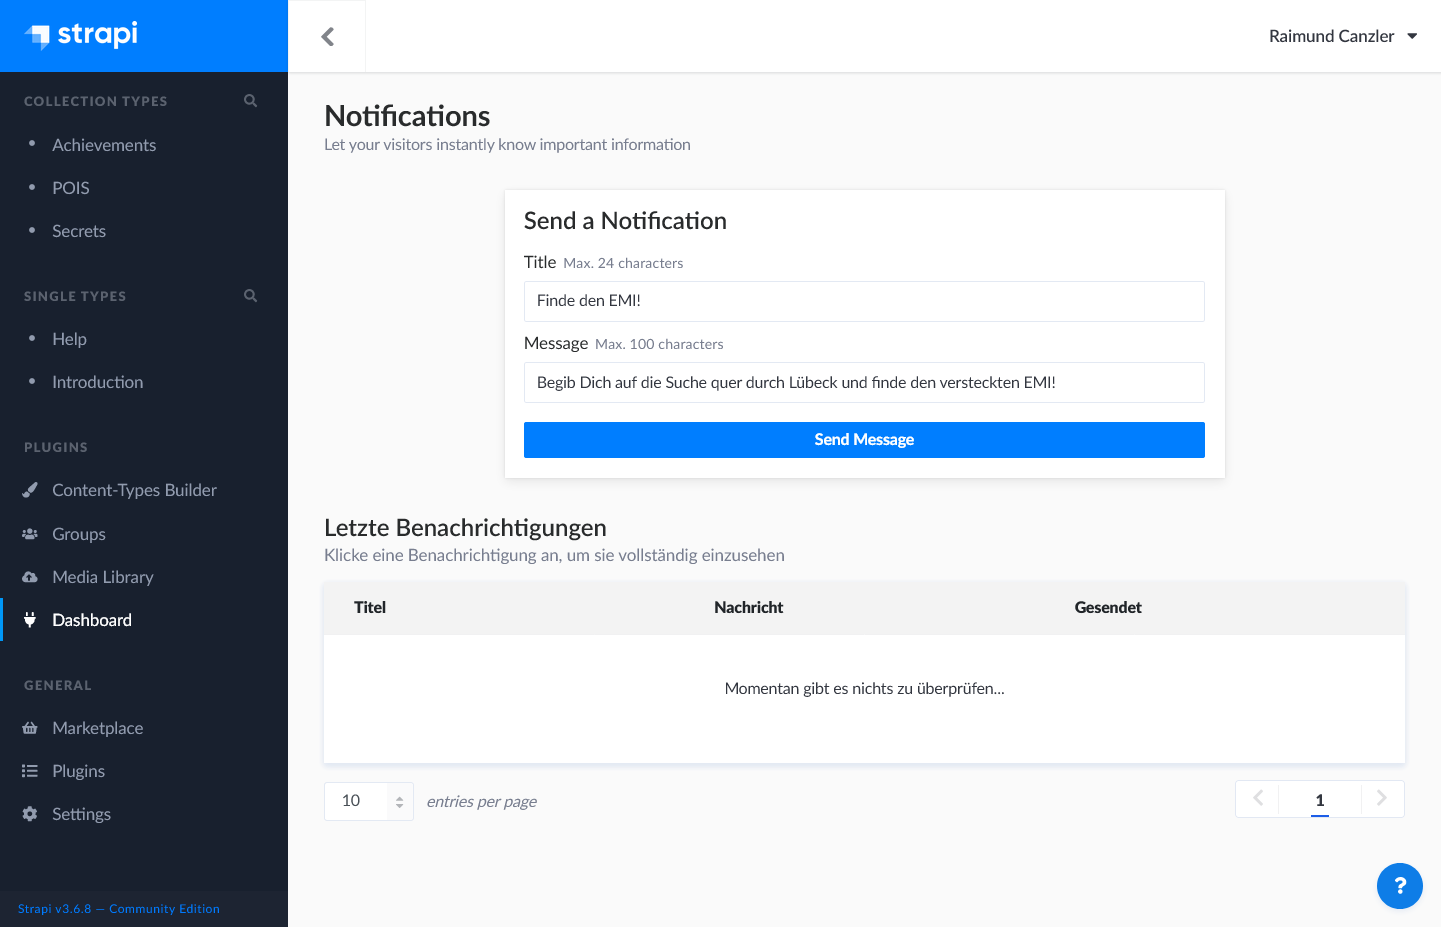
\includegraphics[width=\linewidth]{dialog/dashboard/notifications.png}
    \caption{Dashboard - Übersicht der Benachrichtigungen}
    \label{fig:dialog-v-notifications}
\end{figure}

\begin{figure}[htpb]
    \centering
    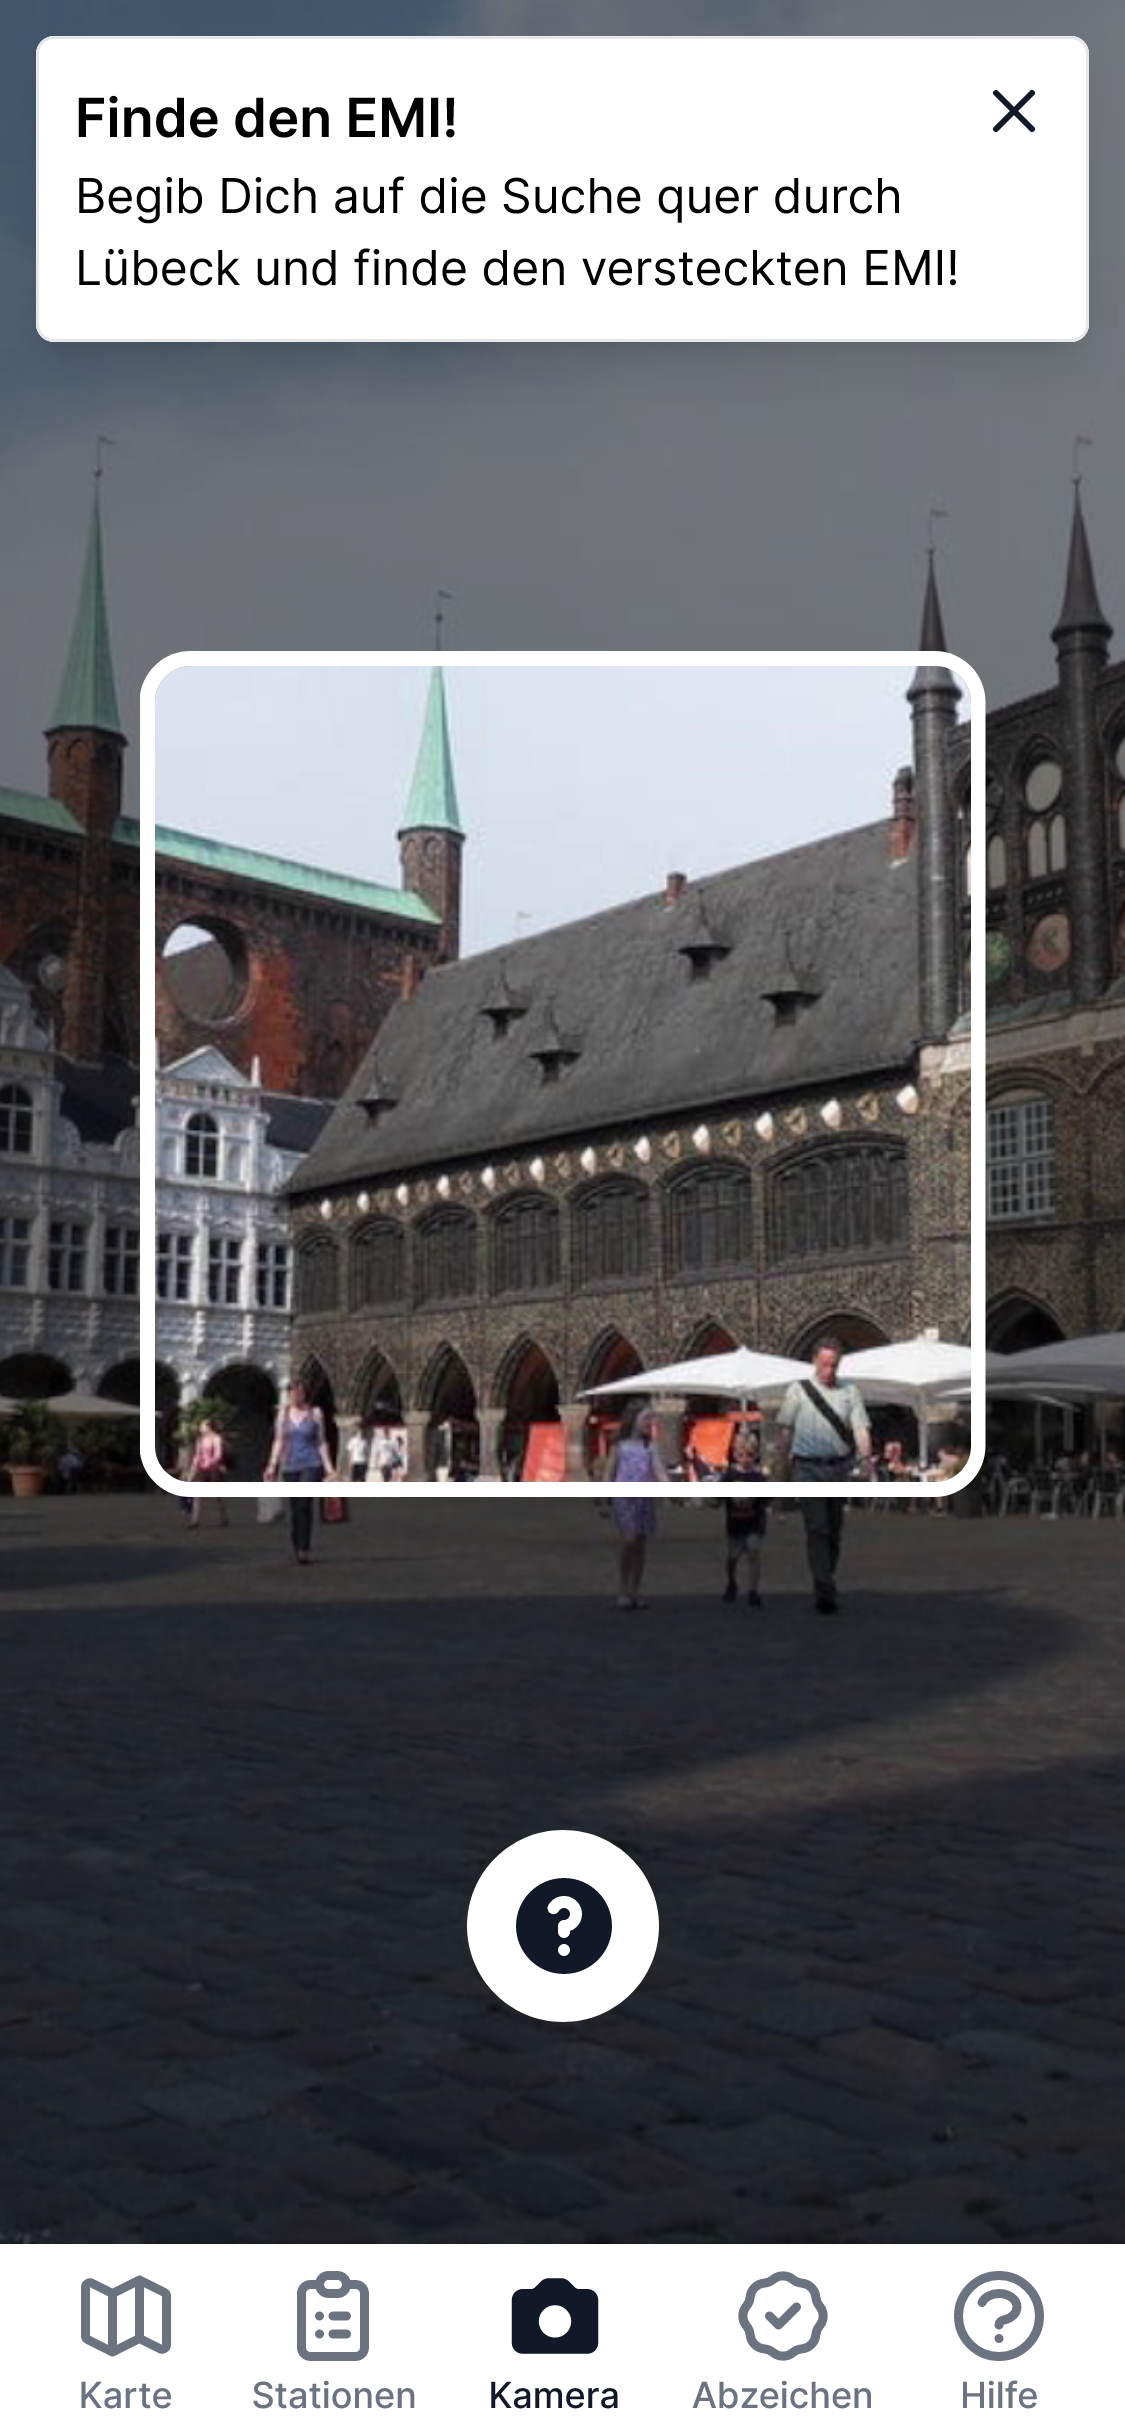
\includegraphics[width=.308\linewidth]{dialog/app/notification.png}
    \caption{Web-App - Erhaltene Benachrichtigung}
    \label{fig:dialog-t-notification}
\end{figure}

Nach einer Weile wird Sven etwas unruhig, da er sich Gedanken macht, ob die
Teilnehmenden an seiner Veranstaltung Spaß haben. Um dem entgegenzuwirken,
schickt Sven eine Feedback-Anfrage auf der Evaluationsseite aus
\autoref{fig:dialog-v-feedback} ab, in welcher er die Teilnehmenden fragt, wie
ihnen die Technology Bits gefallen.

Christina, welche immer noch auf der Suche nach dem EMI ist, sieht in diesem
Moment Svens Feedback-Anfrage als Pop-up auf ihrem Gerät (\autoref{fig:dialog-t-feedback}). Da sie schon eine Weile vergebens auf der
Suche ist, entschließt sie sich dazu, den mittleren Smiley anzutippen und wählt
anschließend Organisation aus.

\begin{figure}[hp]
    \centering
    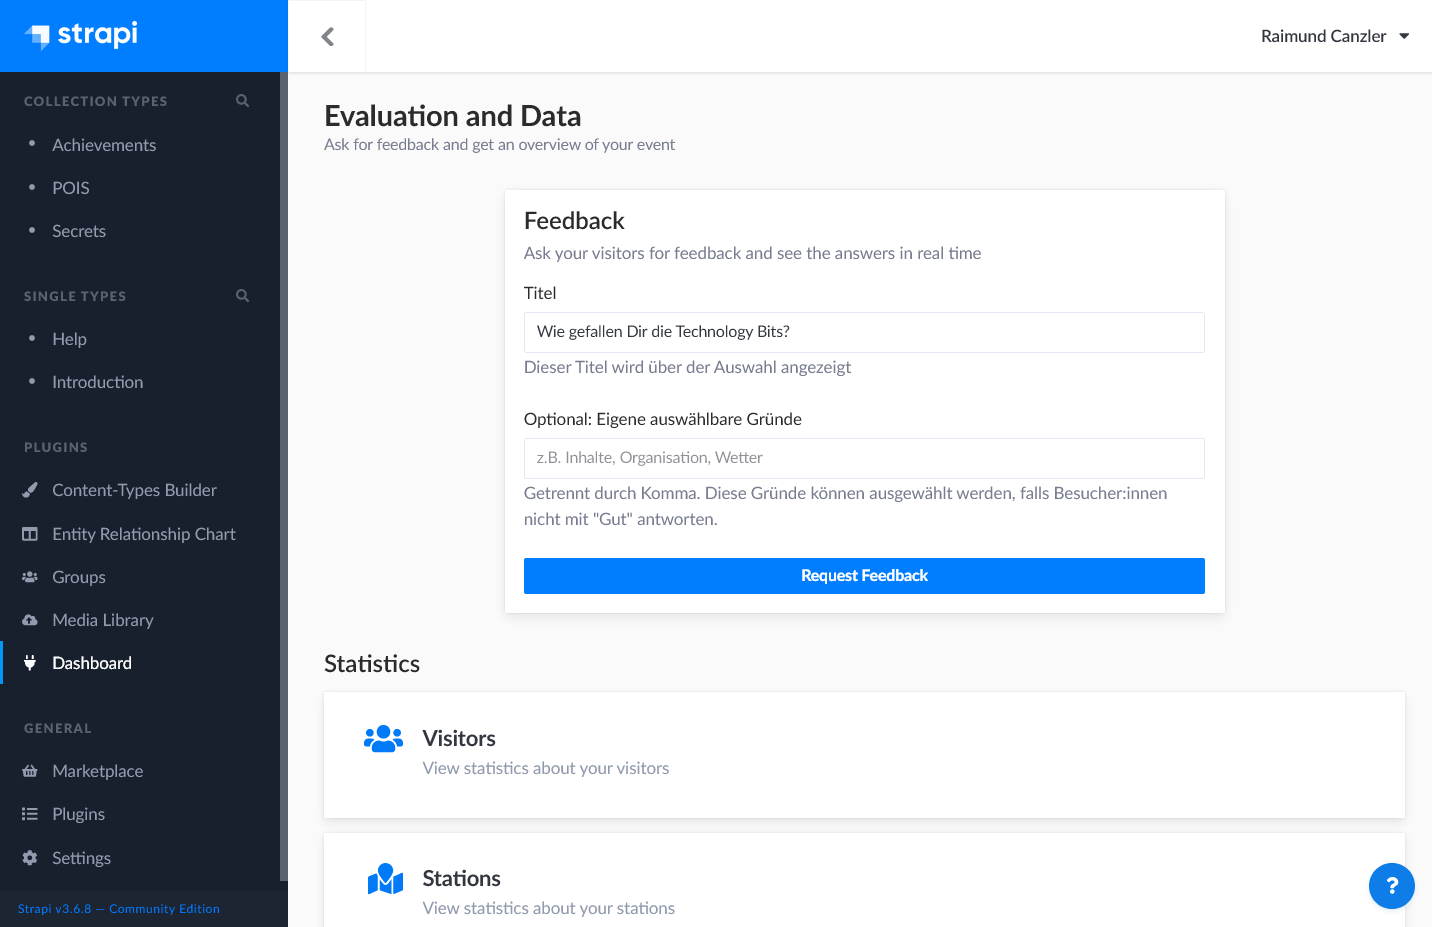
\includegraphics[width=\linewidth]{dialog/dashboard/evaluation_feedback.png}
    \caption{Dashboard - Feedback-Anfrage}
    \label{fig:dialog-v-feedback}
\end{figure}

\begin{figure}[hp]
    \centering
    \begin{minipage}{.5\textwidth}
        \centering
        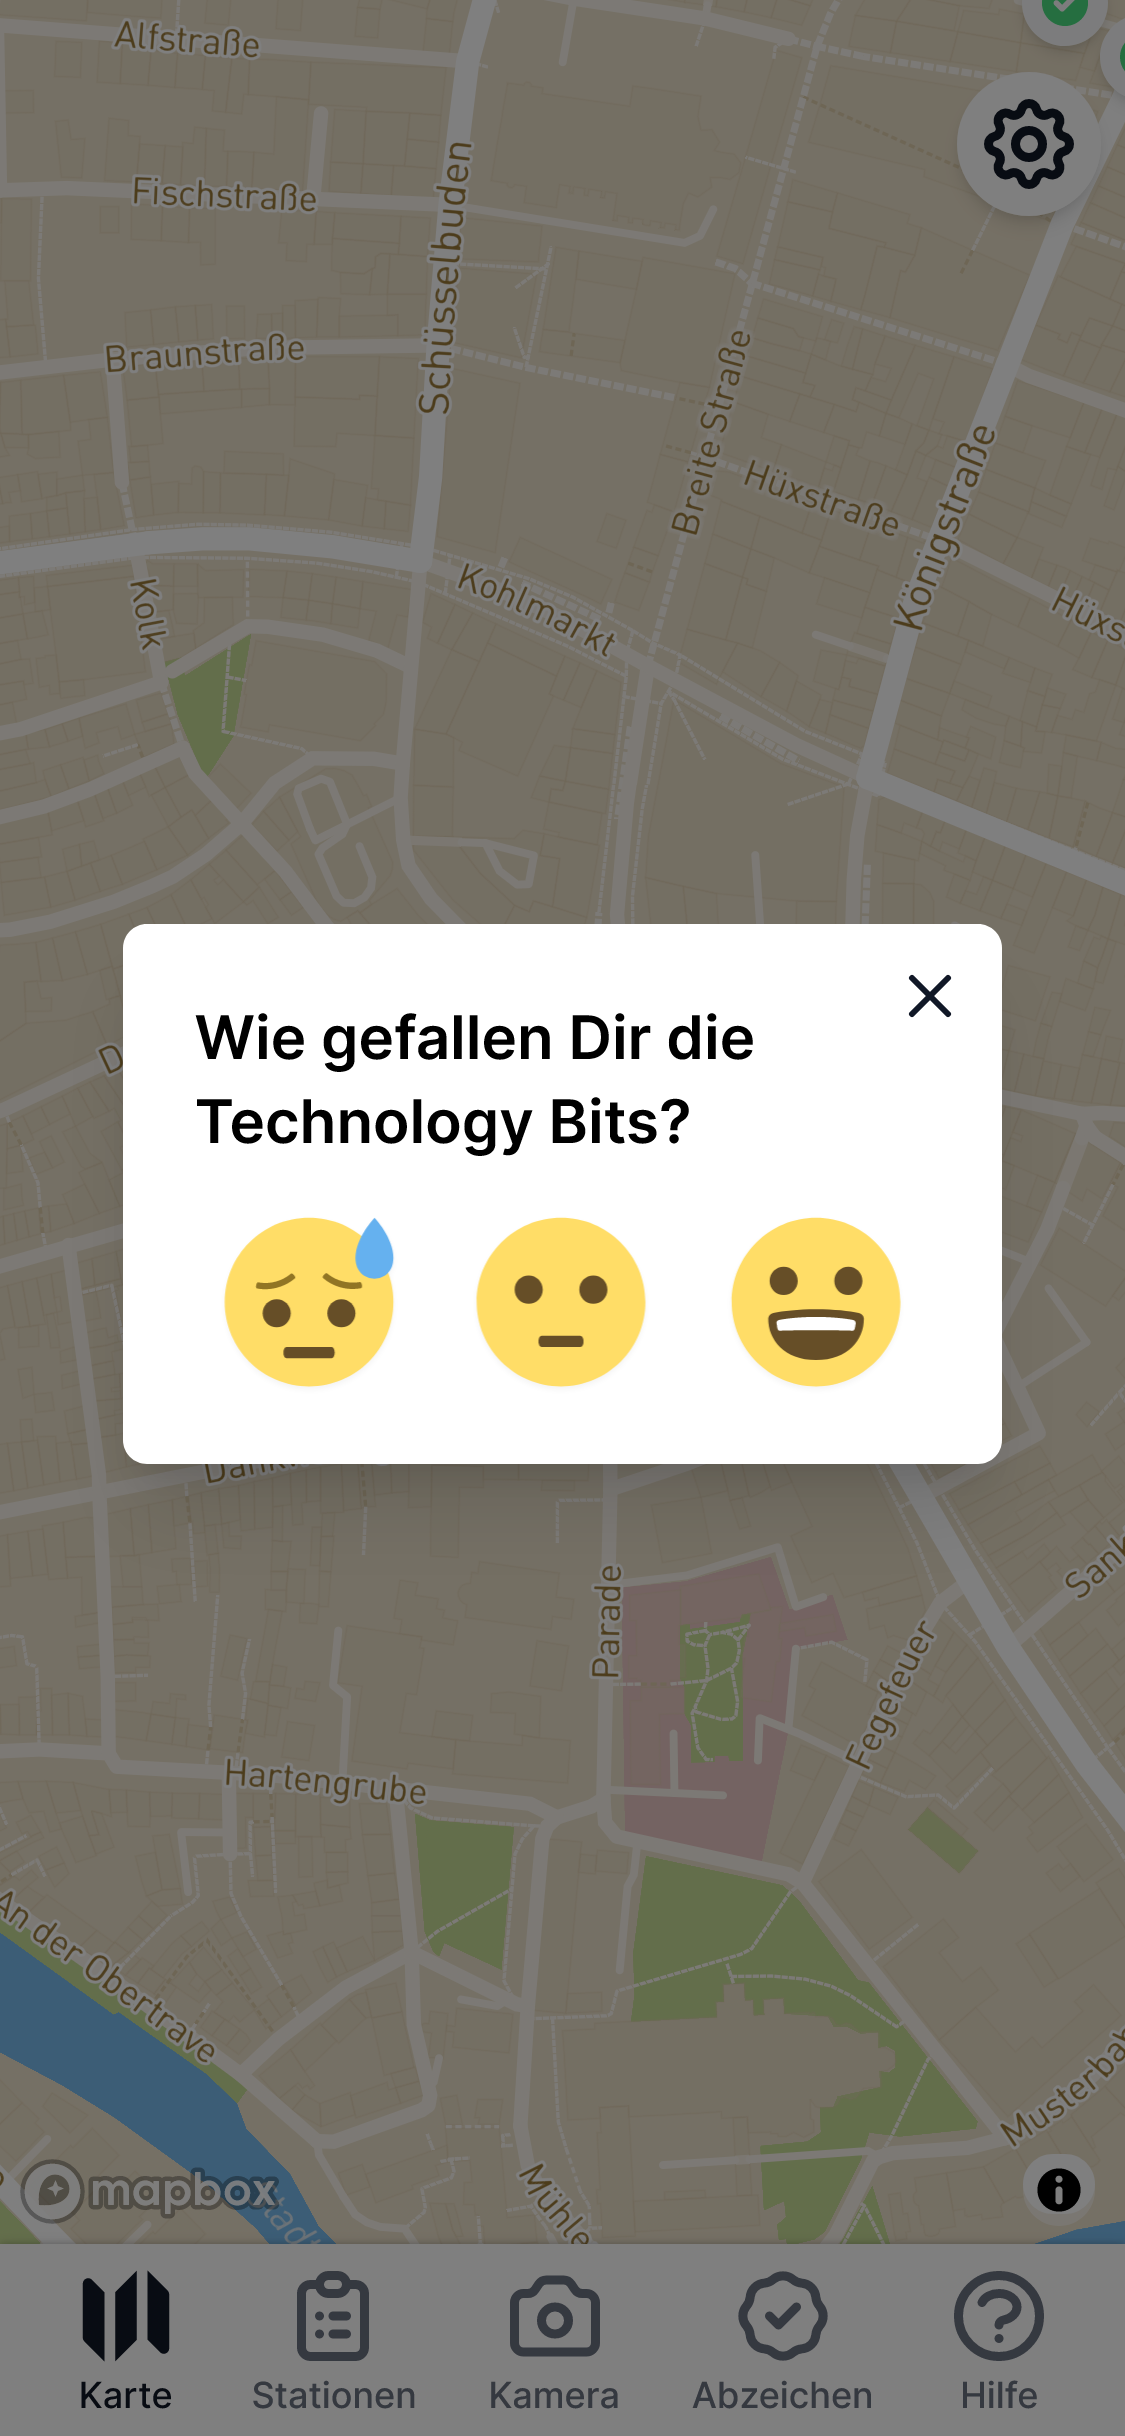
\includegraphics[width=.6\linewidth]{dialog/app/feedback.png}
    \end{minipage}%
    \begin{minipage}{.5\textwidth}
        \centering
        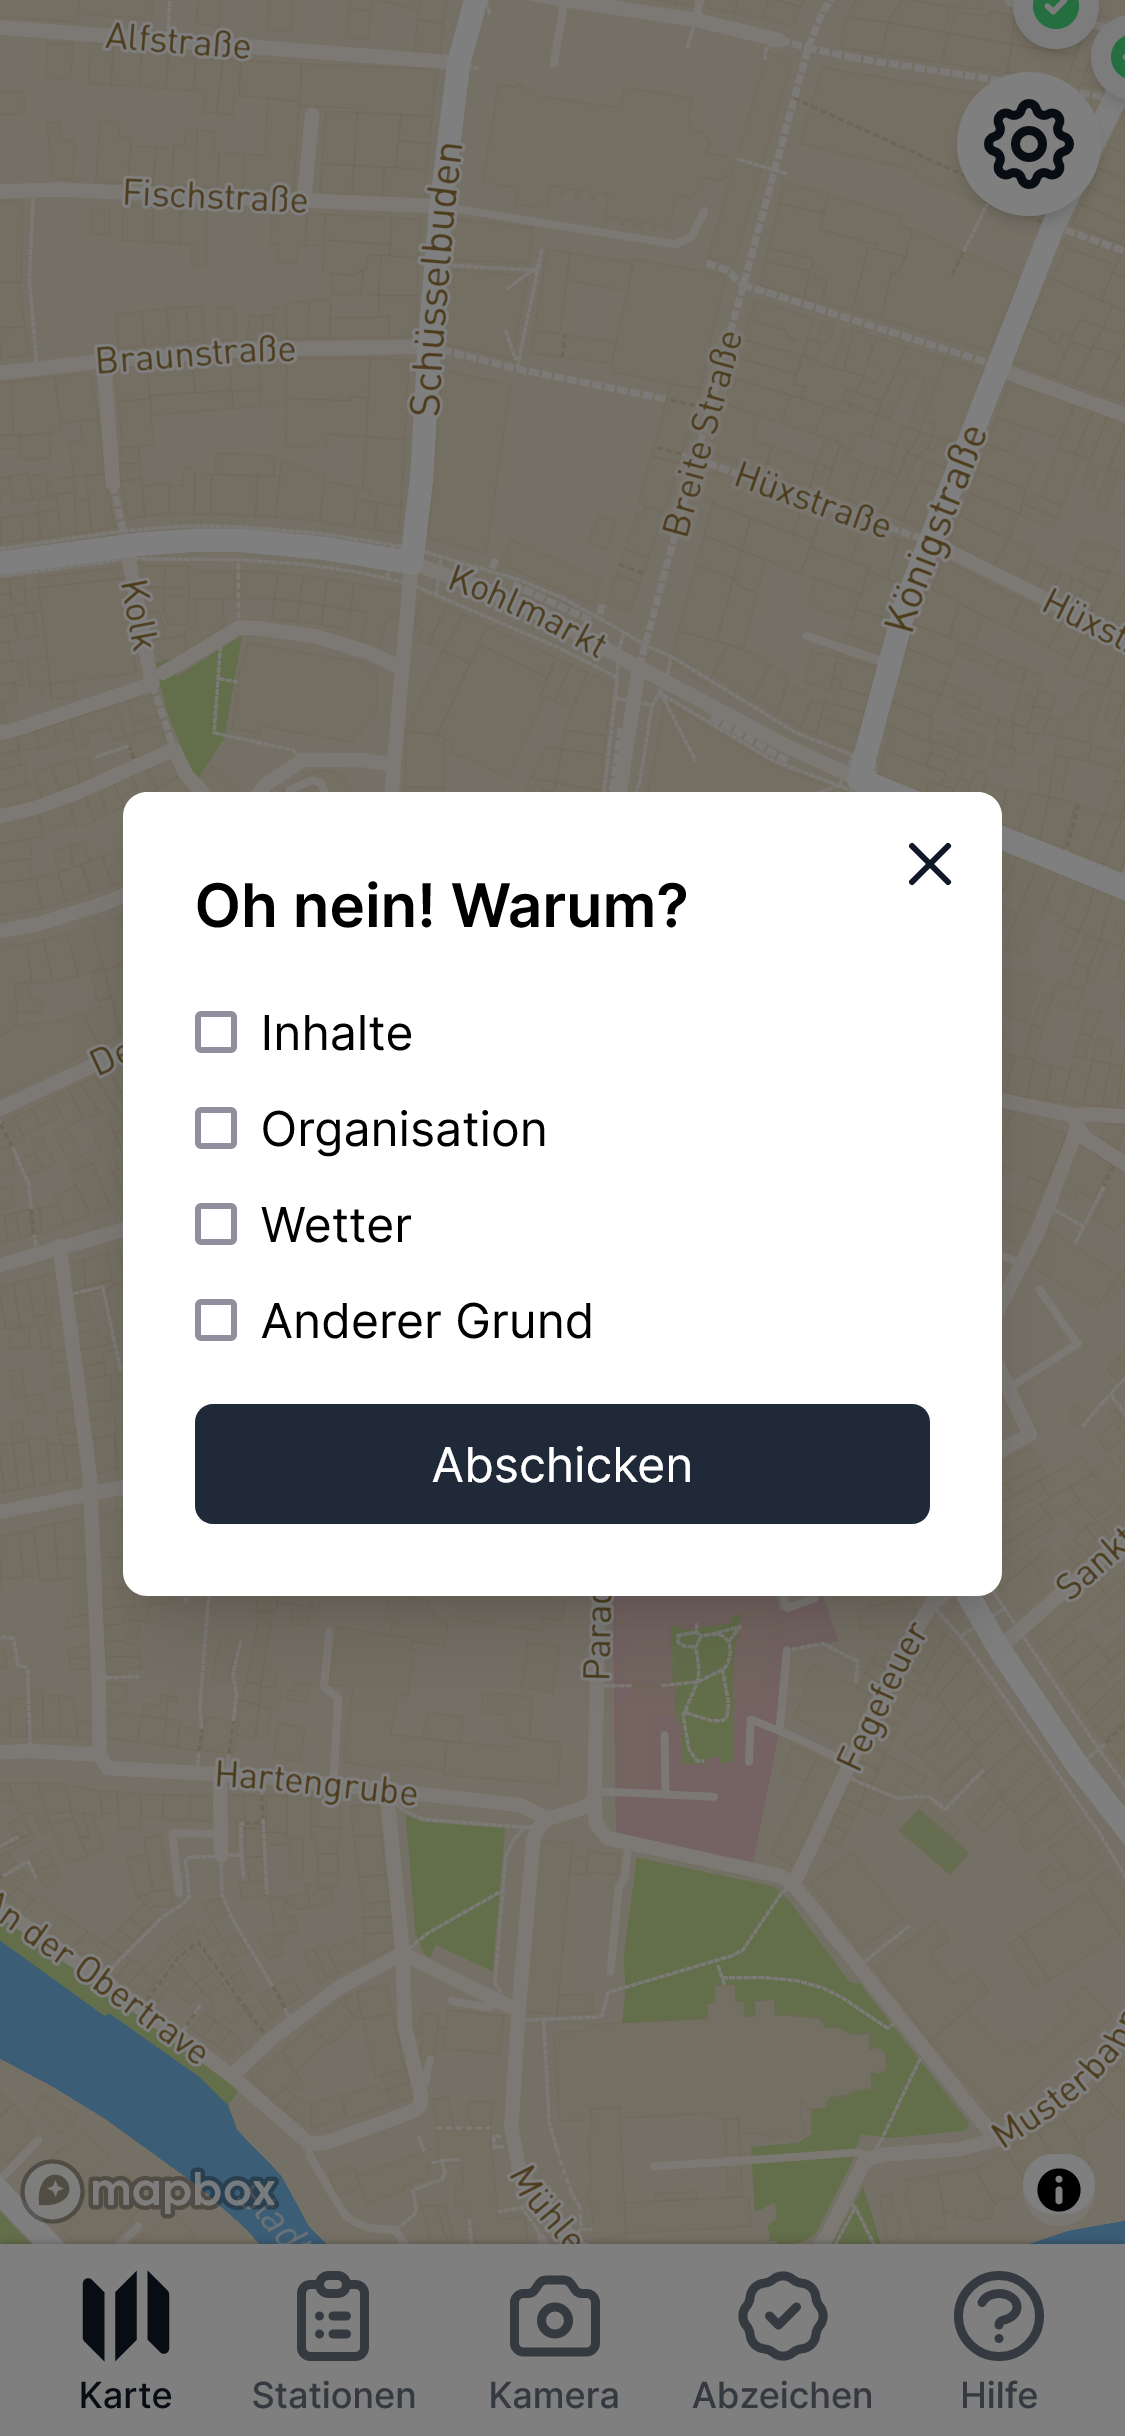
\includegraphics[width=.6\linewidth]{dialog/app/feedback_not_ok.png}
    \end{minipage}
    \caption{Web-App - Feedback}
    \label{fig:dialog-t-feedback}
\end{figure}

Zwischenzeitlich hat Sven die Statistiken auf der „Evaluation und
Statistiken“-Seite aus \autoref{fig:dialog-v-statistics} entdeckt. Dort schaut
er sich nach und nach die Statistiken zu Besuchenden (\autoref{fig:dialog-v-statistics-visitors}), Station (\autoref{fig:dialog-v-statistics-stations}), Abzeichen und Feedback-Anfragen an
(\autoref{fig:dialog-v-statistics-feedback}).

\begin{figure}[hp]
    \centering
    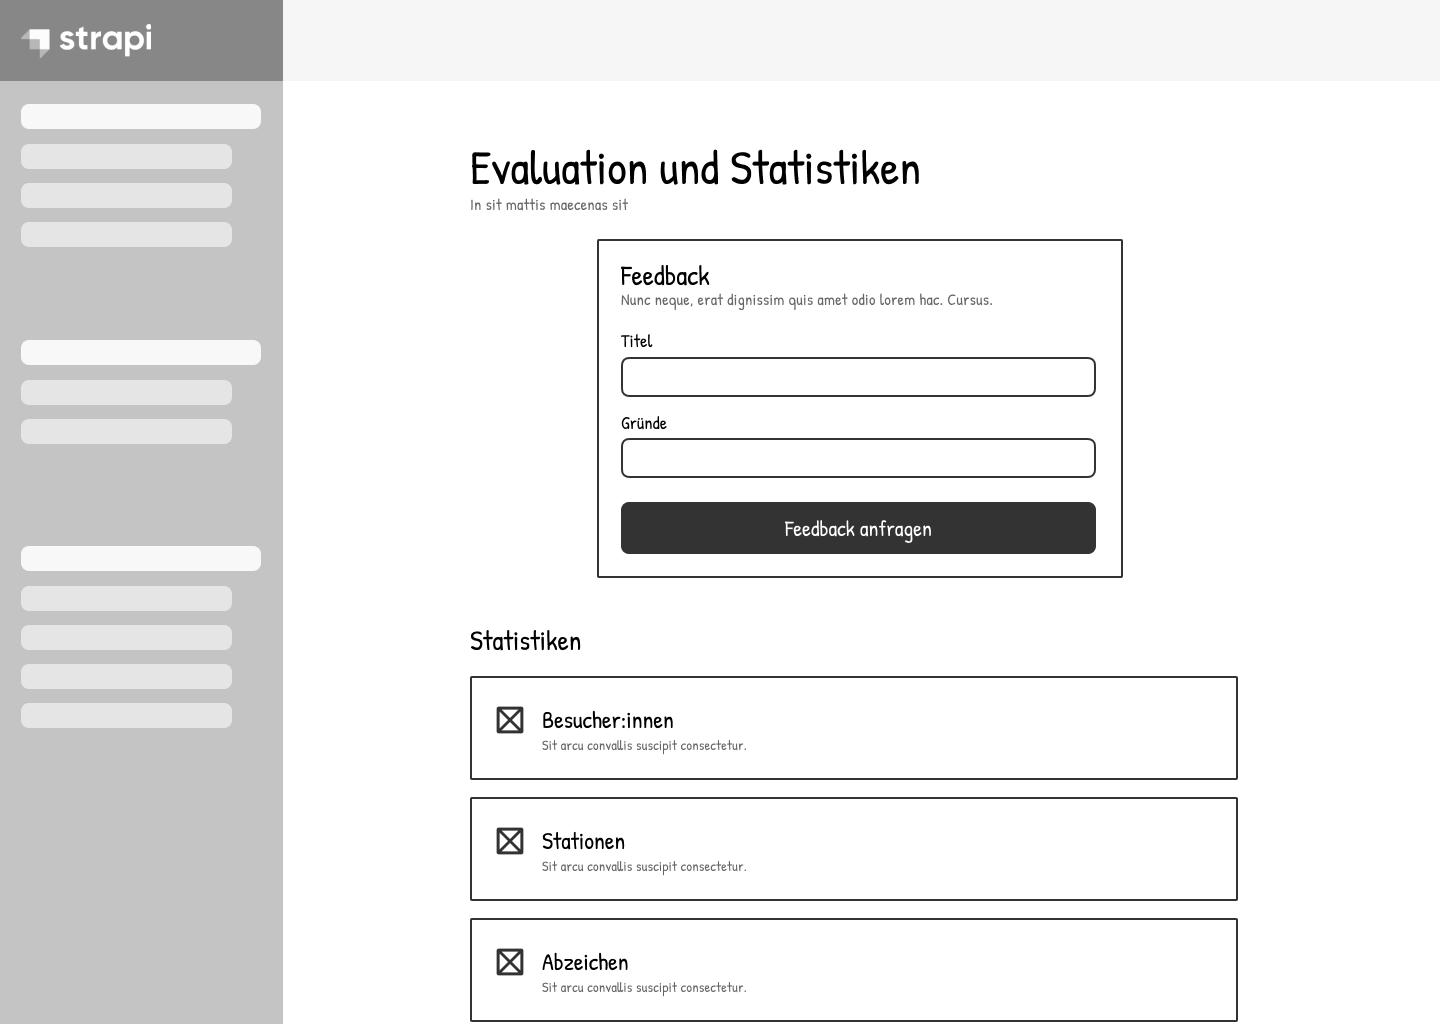
\includegraphics[width=\linewidth]{dialog/dashboard/evaluation_statistics.png}
    \caption{Dashboard - Übersicht der Statistiken}
    \label{fig:dialog-v-statistics}
\end{figure}

\begin{figure}[hp]
    \centering
    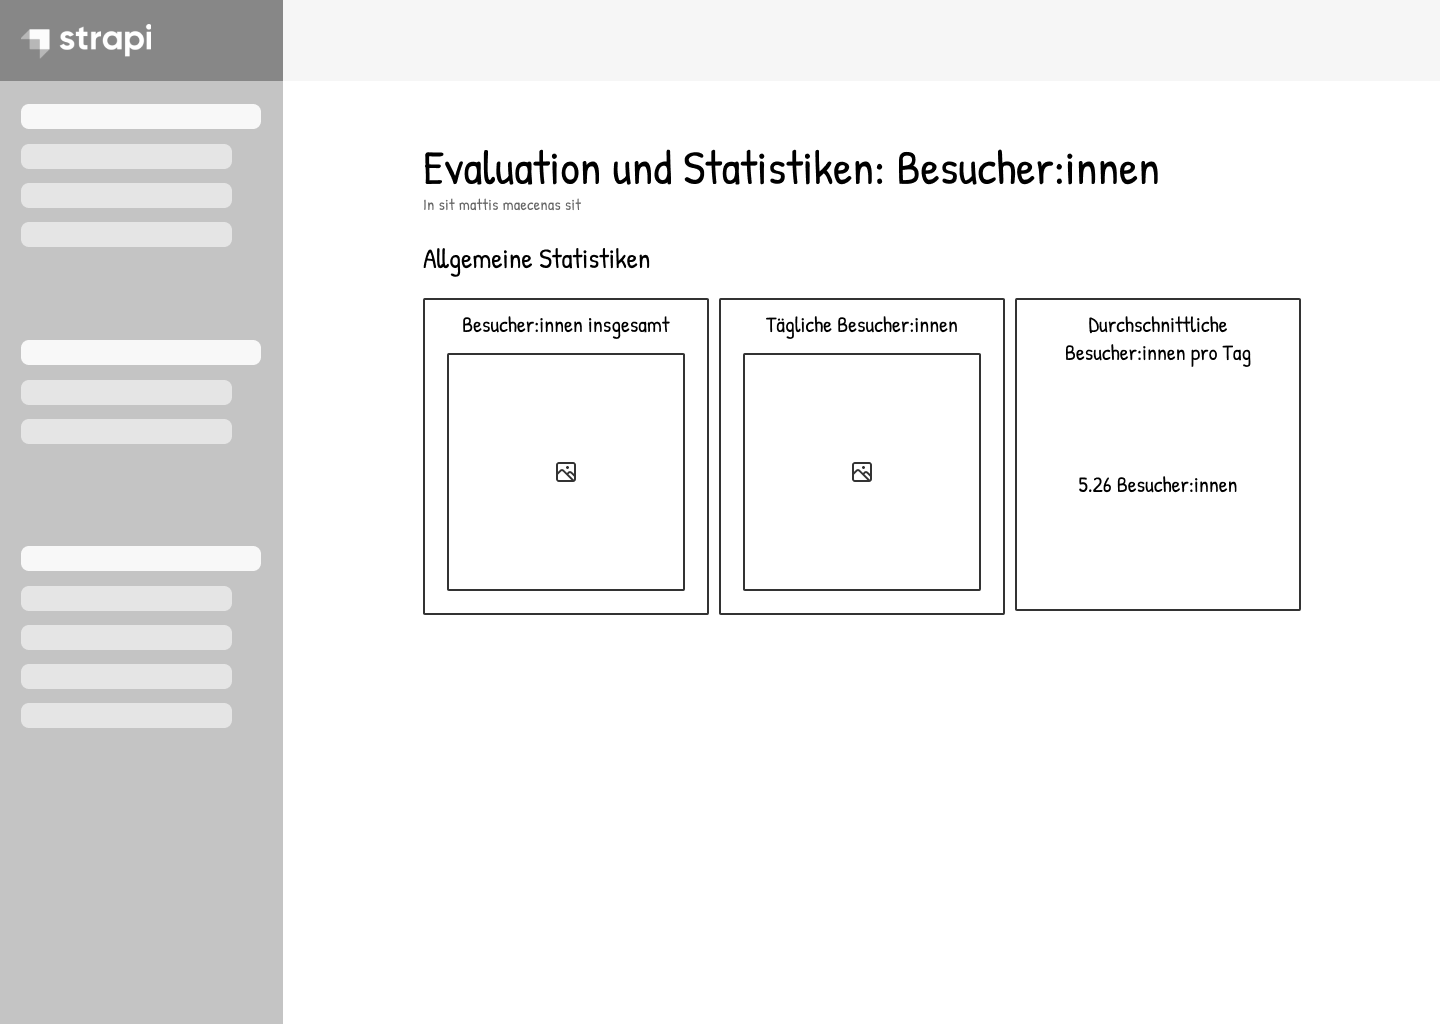
\includegraphics[width=\linewidth]{dialog/dashboard/statistics_visitor.png}
    \caption{Dashboard - Statistiken zu Besuchenden}
    \label{fig:dialog-v-statistics-visitors}
\end{figure}

\begin{figure}[hp]
    \centering
    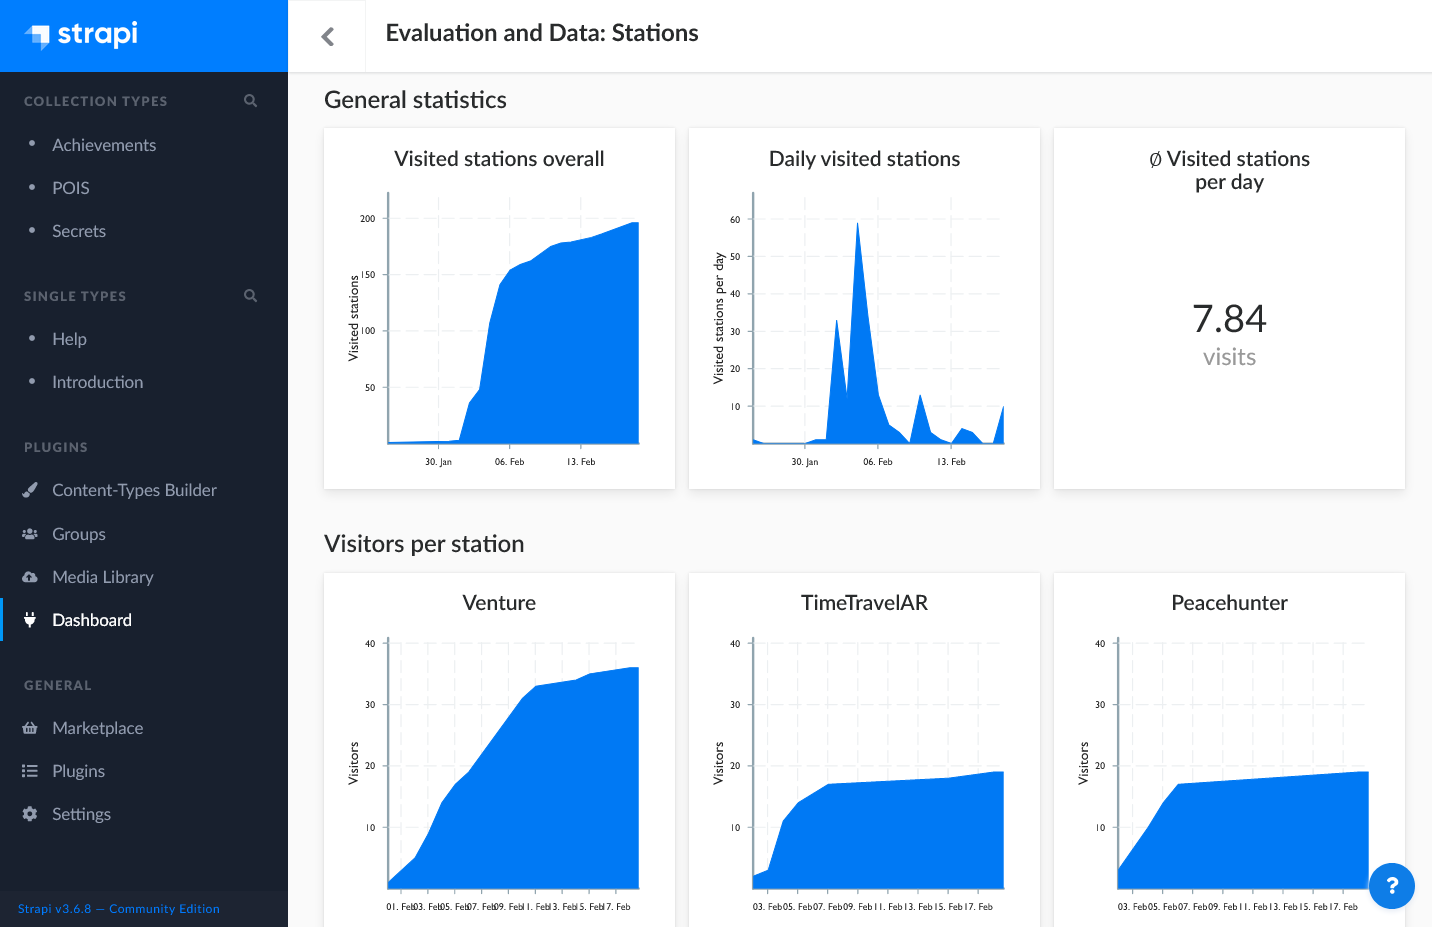
\includegraphics[width=\linewidth]{dialog/dashboard/statistics_station.png}
    \caption{Dashboard - Statistiken zu Stationen}
    \label{fig:dialog-v-statistics-stations}
\end{figure}

\begin{figure}[hp]
    \centering
    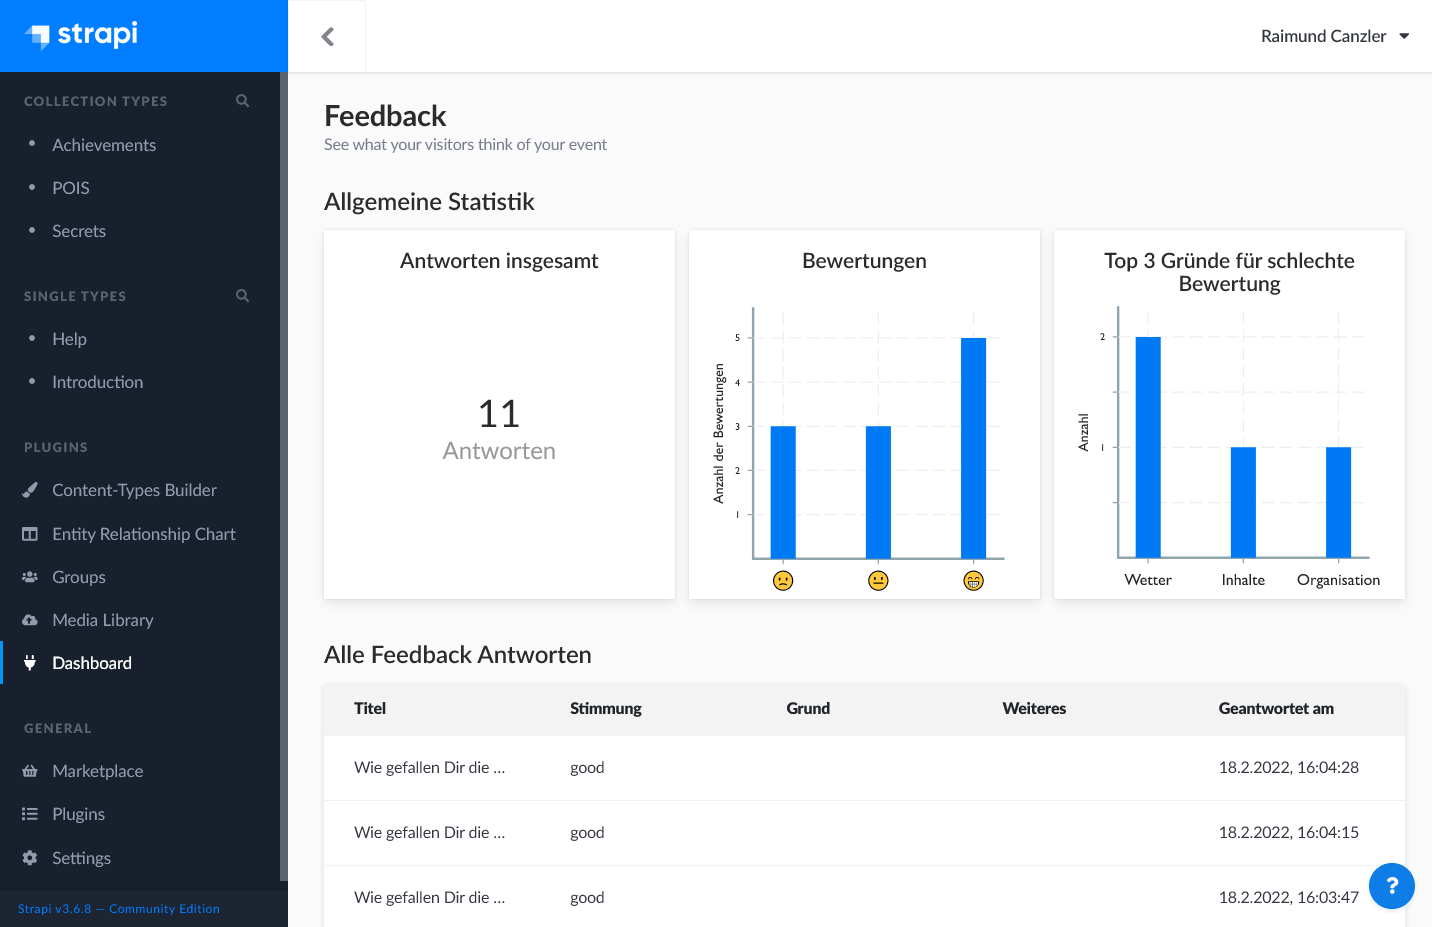
\includegraphics[width=\linewidth]{dialog/dashboard/statistics_feedback.png}
    \caption{Dashboard - Statistiken zu Feedback-Anfragen}
    \label{fig:dialog-v-statistics-feedback}
\end{figure}